%% This is file `elsarticle-template-1-num.tex',
%%
%% Copyright 2009 Elsevier Ltd
%%
%% This file is part of the 'Elsarticle Bundle'.
%% ---------------------------------------------
%%
%% It may be distributed under the conditions of the LaTeX Project Public
%% License, either version 1.2 of this license or (at your option) any
%% later version.  The latest version of this license is in
%%    http://www.latex-project.org/lppl.txt
%% and version 1.2 or later is part of all distributions of LaTeX
%% version 1999/12/01 or later.
%%
%% The list of all files belonging to the 'Elsarticle Bundle' is
%% given in the file `manifest.txt'.
%%
%% Template article for Elsevier's document class `elsarticle'
%% with numbered style bibliographic references
%%
%% $Id: elsarticle-template-1-num.tex 149 2009-10-08 05:01:15Z rishi $
%% $URL: http://lenova.river-valley.com/svn/elsbst/trunk/elsarticle-template-1-num.tex $
%%
%%\documentclass[preprint,12pt]{elsarticle}

%% Use the option review to obtain double line spacing
%% \documentclass[preprint,review,12pt]{elsarticle}

%% Use the options 1p,twocolumn; 3p; 3p,twocolumn; 5p; or 5p,twocolumn
%% for a journal layout:
%% \documentclass[final,1p,times]{elsarticle}
%% \documentclass[final,1p,times,twocolumn]{elsarticle}
%% \documentclass[final,3p,times]{elsarticle}
 \documentclass[final,3p,times,twocolumn]{elsarticle}
%% \documentclass[final,5p,times]{elsarticle}
%% \documentclass[final,5p,times,twocolumn]{elsarticle}

%% if you use PostScript figures in your article
%% use the graphics package for simple commands
%% \usepackage{graphics}
%% or use the graphicx package for more complicated commands
%% \usepackage{graphicx}
%% or use the epsfig package if you prefer to use the old commands
%% \usepackage{epsfig}

%% The amssymb package provides various useful mathematical symbols
\usepackage{amssymb}
%% The amsthm package provides extended theorem environments
%% \usepackage{amsthm}

%% The lineno packages adds line numbers. Start line numbering with
%% \begin{linenumbers}, end it with \end{linenumbers}. Or switch it on
%% for the whole article with \linenumbers after \end{frontmatter}.
%% \usepackage{lineno}

%% natbib.sty is loaded by default. However, natbib options can be
%% provided with \biboptions{...} command. Following options are
%% valid:

%%   round  -  round parentheses are used (default)
%%   square -  square brackets are used   [option]
%%   curly  -  curly braces are used      {option}
%%   angle  -  angle brackets are used    <option>
%%   semicolon  -  multiple citations separated by semi-colon
%%   colon  - same as semicolon, an earlier confusion
%%   comma  -  separated by comma
%%   numbers-  selects numerical citations
%%   super  -  numerical citations as superscripts
%%   sort   -  sorts multiple citations according to order in ref. list
%%   sort&compress   -  like sort, but also compresses numerical citations
%%   compress - compresses without sorting
%%
%% \biboptions{comma,round}

% \biboptions{}

% HPS stuff
\usepackage{color}
%\usepackage{multicol}
\newcommand{\Aprime}{A\ensuremath{^\prime}}
\newcommand{\ee}{e$^+$e$^-$}
\newcommand{\fluenceunit}{1~MeV~neutron~equivalent/cm\ensuremath{^2}}
\newcommand{\geant}{{\sc Geant4}}
\newcommand{\egs}{{\sc EGS5}}
\newcommand{\moliere}{Moli\`{e}re}
%\include{affiliations}

\journal{Nuclear Physics B}

\begin{document}

\begin{frontmatter}

%% Title, authors and addresses

%% use the tnoteref command within \title for footnotes;
%% use the tnotetext command for the associated footnote;
%% use the fnref command within \author or \address for footnotes;
%% use the fntext command for the associated footnote;
%% use the corref command within \author for corresponding author footnotes;
%% use the cortext command for the associated footnote;
%% use the ead command for the email address,
%% and the form \ead[url] for the home page:
%%
%% \title{Title\tnoteref{label1}}
%% \tnotetext[label1]{}
%% \author{Name\corref{cor1}\fnref{label2}}
%% \ead{email address}
%% \ead[url]{home page}
%% \fntext[label2]{}
%% \cortext[cor1]{}
%% \address{Address\fnref{label3}}
%% \fntext[label3]{}

\title{The Heavy Photon Search Test Detector}


%%%%%%%%%%%%%%%%%%%%%%%%%%%%%%%%%%%%%%%%%%%%%%%%%%
%% use optional labels to link authors explicitly to addresses:
%% \author[label1,label2]{<author name>}
%% \address[label1]{<address>}
%% \address[label2]{<address>}


\newcommand{\red[1]}{{\color{red}{\bf #1}}}
\newcommand{\JLAB}{Thomas Jefferson National Accelerator Facility, Newport News, Virginia 23606}
\newcommand{\CUA}{Catholic University of America, Washington, D.C. 20064}
\newcommand{\OU}{Ohio University,  Athens, Ohio 45701}
\newcommand{\YEREVAN}{Yerevan Physics Institute, 375036 Yerevan, Armenia}
\newcommand{\SCAROLINA}{University of South Carolina, Columbia, South Carolina 29208}
\newcommand{\NSU}{Norfolk State University, Norfolk, Virginia 23504}
\newcommand{\ODU}{Old Dominion University, Norfolk, Virginia 23529}
\newcommand{\genova}{Istituto Nazionale di Fisica Nucleare, Sezione di Genova e Dipartimento di Fisica dell\'Universita, 16146 Genova, Italy}
\newcommand{\SACLAY}{CEA, Centre de Saclay, Irfu/Service de Physique Nucl\'eaire 91191 Gif-sur-Yvette, France}
\newcommand{\ORSAY}{Institut de Physique Nucleaire d'Orsay, IN2P3, BP 1, 91406 Orsay, France}
\newcommand{\ECOLE}{CPhT, Ecole Polytechnique, F 91128 PALAISEAU CEDEX, France}
\newcommand{\UCSC}{University of California, Santa Cruz, CA 95064}
\newcommand{\SUNY}{Stony Brook University, Stony Brook, NY 11794-3800}
\newcommand{\FNAL}{Fermi National Accelerator Laboratory, Batavia, IL 60510-5011}
\newcommand{\UNH}{University of New Hampshire, Department of Physics, Durham, NH 03824}
\newcommand{\PERIMETER}{Perimeter Institute, Ontario, Canada N2L 2Y5}
\newcommand{\RPI}{Rensselaer Polytechnic Institute, Department of Physics, Troy, NY 12181}
\newcommand{\SLAC}{SLAC National Accelerator Laboratory, Menlo Park, CA 94025}
\newcommand{\WNM}{The College of William and Mary, Department of Physics, Williamsburg, VA 23185}


\author[SLAC]{C. Field}
\author[SLAC]{P. Hansson Adrian\corref{corrauthor}}
\author[SLAC]{N. Graf} 
\author[SLAC]{ M. Graham} 
\author[SLAC]{ G. Haller} 
\author[SLAC]{ R. Herbst} 
%\author[SLAC]{ J. Jaros\corref{spoks}} 
\author[SLAC]{ J. Jaros}
\author[SLAC]{T. Maruyama} 
\author[SLAC]{ J. McCormick} 
\author[SLAC]{ K. Moffeit} 
\author[SLAC]{ T. Nelson} 
\author[SLAC]{ H. Neal} 
\author[SLAC]{ A. Odian} 
\author[SLAC]{ M. Oriunno} 
\author[SLAC]{ S. Uemura} 
\author[SLAC]{ D. Walz}
%
\author[UCSC]{A. Grillo} 
\author[UCSC]{ V. Fadeyev} 
\author[UCSC]{ O. Moreno}
%
\author[FNAL]{W. Cooper}
%
\author[JLAB]{S. Boyarinov} 
\author[JLAB]{ V. Burkert} 
\author[JLAB]{ A. Deur} 
\author[JLAB]{ H. Egiyan}
 \author[JLAB]{ L. Elouadrhiri} 
 \author[JLAB]{ A. Freyberger} 
 \author[JLAB]{ F.-X. Girod} 
 \author[JLAB]{ V. Kubarovsky} 
\author[JLAB]{ Y. Sharabian} 
%\author[JLAB]{ S. Stepanyan\corref{spoks}} 
\author[JLAB]{ S. Stepanyan}
\author[JLAB]{ M. Ungaro} 
\author[JLAB]{ B. Wojtsekhowski}
%
\author[SUNY]{R. Essig}
%
%\author[UNH]{M. Holtrop\corref{spoks}} 
\author[UNH]{M. Holtrop}
\author[UNH]{ K. Slifer} 
\author[UNH]{ S. K. Phillips}
%
\author[ORSAY]{A. Fradi} 
\author[ORSAY]{ B. Guegan} 
\author[ORSAY]{ M. Guidal} 
\author[ORSAY]{ S. Niccolai} 
\author[ORSAY]{ S. Pisano} 
\author[ORSAY]{ E. Rauly}
\author[ORSAY]{ P. Rosier}
\author[ORSAY]{D. Sokhan}
 %
\author[PERIMETER]{P. Schuster} 
\author[PERIMETER]{ N. Toro}
%
\author[YEREVAN]{N. Dashyan} 
\author[YEREVAN]{ N. Gevorgyan} 
\author[YEREVAN]{ R. Paremuzyan}
\author[YEREVAN]{ H. Voskanyan}
%
\author[NSU]{M. Khandaker} 
\author[NSU]{ C. Salgado}
%
\author[GENOVA]{M. Battaglieri} 
\author[GENOVA]{ R. De Vita}
%
\author[ODU]{S. Bueltmann} 
\author[ODU]{ L. Weinstein}
%
\author[RPI]{P. Stoler} 
\author[RPI]{A. Kubarovsky}
%
\author[WNM]{K. Griffioen}

\address[SLAC]{\SLAC}                                 
\address[UCSC]{\UCSC}
\address[FNAL]{\FNAL}
\address[JLAB]{\JLAB}
\address[SUNY]{\SUNY}
\address[UNH]{\UNH}
\address[ORSAY]{\ORSAY}
\address[PERIMETER]{\PERIMETER}
\address[YEREVAN]{\YEREVAN}
\address[NSU]{\NSU}
\address[GENOVA]{\genova}
\address[ODU]{\ODU}
\address[RPI]{\RPI}
\address[WNM]{\WNM}

 %\cortext[spoks]{Co-spokesperson}

\cortext[corrauthor]{Corresponding author. \ead{phansson@slac.stanford.edu}}





%\author[label1]{Per Ledin}
%\ead{contact@hps.discovery.com}
%\author[slac]{Per Hansson Adrian\corref{cor1}}
%\ead{phansson@slac.stanford.edu}
%\author[slac]{Timothy K. Nelson}
%\address[slac]{SLAC National Accelerator Laboratory, 94025, Menlo Park, CA, USA}
%\address[label1]{Lule\aa~Hockey}

%%%%%%%%%%%%%%%%%%%%%%%%%%%%%%%%%%%%%%%%%%%%%%%%%%



\begin{abstract}
Construction and design of the Heavy Photon Search (HPS) experiment, designed to search for an 
\ee resonance from heavy photon production in a fixed-target setup at the Thomas Jefferson 
Accelerator Facility (JLab), is ongoing. As a first stage, a test apparatus was constructed and 
operated at JLab to demonstrate that the apparatus and data acquisition systems are technically 
feasible and that the trigger rates and occupancies encountered in electron-beam running are as 
simulated. Given dedicated running time with electron beams, the HPS Test apparatus is 
capable of searching for heavy photons in unexplored regions of parameter space.  Charged 
particle tracks are measured with a compact forward silicon microstrip detector and 
electromagnetic showers from electrons and photons are detected in a dense array of 
PbWO$_{4}$ crystals. To allow clean passage of the scattered intense electron beam after 
the thin tungsten target foil while keeping sensitivity to low-mass heavy photons,  the sensitive region 
of the detectors are place at $\pm 15$~mrad with respect to the horizontal beam plane. 
The discrimination between prompt and displaced \ee pairs requires the first layer of silicon 
sensors to be placed only 10~cm behind the target and 0.5~mm from the beam. 
The HPS Test apparatus included the high-speed trigger and data acquisition needed for 
running with electron beams. Details of the layout and performance of the Test detectors and 
associated readout electronics are presented. 
\end{abstract}

\begin{keyword}
%% keywords here, in the form: keyword \sep keyword
silicon microstrip \sep tracking  \sep vertexing \sep heavy photon \sep dark photon \sep hidden sector \sep electromagnetic calorimeter
%% MSC codes here, in the form: \MSC code \sep code
%% or \MSC[2008] code \sep code (2000 is the default)

\end{keyword}

\end{frontmatter}

\clearpage
\tableofcontents
\clearpage
\newpage
\newpage

%%
%% Start line numbering here if you want
%%
% \linenumbers

%% main text
\section{Introduction}
\label{introduction}
Heavy photons, aka "hidden sector" or "dark" photons, or from here on \Aprime{}, are particles with 
mass $10-1000$~MeV 
which couple weakly to the Standard Model photon~\cite{Holdom:1985ag}, so can be radiated by 
electrons, and can decay 
into \ee pairs, albeit at rates far below those of QED trident processes. They have been suggested by 
numerous Beyond Standard Model theories and as an explanation of the current muonic $g-2$ 
anomaly, and may couple directly to hidden sector particles that may constitute all or some of the 
dark matter~\cite{ArkaniHamed:2008qn}. 
Current phenomenology highlights the $20-1000$~MeV/c$^{2}$ mass range, and 
suggests that \Aprime's couple to electric charge with strength $\epsilon$e, where 
$\epsilon$ is in the range of $10^{-3} -10^{-5}$. [REFERENCE]. This range of parameters makes 
\Aprime{} searches viable in moderate energy fixed target 
electroproduction~\cite{Bjorken:2009mm}, but require large data sets and good mass resolution
to identify a small mass peak above the copious QED background at very small production 
angles. At small couplings, \Aprime's become long-lived, so detection of a displaced decay 
vertex can reject the prompt QED background and boost experimental sensitivity.  These production 
and kinematics poses stringent constraint on the detector requirements:
\begin{itemize}
\item large and uniform acceptance in the forward region close to the beam in order to catch boosted 
\Aprime{} decay products,
\item beam passage through the apparatus in vacuum, to eliminate direct interactions with the 
detector and minimize beam gas interactions, 
\item a flexible, redundant and efficient trigger selecting electron and positron pairs at rates up to 
50~kHz,
\item excellent track reconstruction efficiency for electrons and positrons,
\item good angular and momentum resolution to reconstruct invariant mass precisely,
\item excellent vertex resolution to discriminate displaced \Aprime{} decays from prompt QED 
backgrounds,
\item high rate electronics with excellent timing resolution to minimize out of time backgrounds,
\item data handling rates of 100~MB/s to permanent storage,
\item detector components that can survive and efficiently operate in a high radiation environment 
with local doses exceeding $100$~Mrad.
\end{itemize}
The HPS experiment~\cite{HPS_proposal_2010} uses both invariant mass and 
vertex signatures by placing a $\approx 1$~m long silicon tracking and vertexing detector 10~cm 
downstream  of a 0.25\%~$\chi_0$ tungsten target inside a dipole magnet. The experiment runs at high 
rates (up to 50kHz), exploiting the 
100\% duty cycle of the Thomas Jefferson National Accelerator Facility (JLab) CEBAF accelerator to 
accumulate the need statistics. The trigger is provided by a fast electromagnetic calorimeter just 
downstream of the tracking detector. 


The HPS Test apparatus, a simplified version of the full HPS experiment, was proposed and 
approved at Thomas Jefferson National Accelerator Facility (JLab) as the first stage of the HPS 
experiment. Its purposes included demonstrating that the apparatus and data acquisition systems are 
technically feasible and that the trigger rates and occupancies encountered in electron-beam 
running are as simulated. Given dedicated running time with electron beams, the HPS Test Run 
apparatus is capable of searching for heavy photons in unexplored regions of parameter space.    
The HPS Test apparatus was installed on April 19, 2012, and ran parasitically with the HDice 
experiment~\cite{HDice}, using its photon beam, until May 18. The JLab run schedule 
precluded any dedicated electron beam running, but the HPS Test Run was allowed a short and 
valuable dedicated run with the photon beam. Most technologies used in the Test apparatus will 
be used in the HPS detector with some improvements to each of the systems; both from lessons 
learned during running of the Test run but also from less schedule and budget constraints. 

This paper reviews the HPS Test Run apparatus; documents the performance of the trigger, 
data acquisition, silicon tracking detector, and the electromagnetic calorimeter at the level assumed 
in calculating the physics reach of the HPS experiment. 




%Of particular importance, data from the dedicated photon beam running has been used to 
%compare the measured trigger rates with those expected in simulation. The Test Run trigger rate is 
%almost entirely due to photons which have converted to \ee pairs in a thin target upstream of HPS 
%and it 
%is sensitive to their multiple Coulomb scattering in the conversion target.  During electron beam 
%running, 
%the tails of the multiply Coulomb scattered primary beam are the dominant source of occupancy in %the 
%tracker and trigger rate in the electromagnetic calorimeter. 
%The trigger rates in the Test Run are also sensitive to the tails of the multiple Coulomb
%scattering distribution. Good agreement between the measured and simulated rates confirms
%our understanding of multiple Coulomb scattering and 
%the reliability of the background simulation used to benchmark the physics reach of the HPS 
%experiment. 





\section{Detector Overview}
\label{detector}
\begin{center}
{\small
\begin{figure*}[ht]
    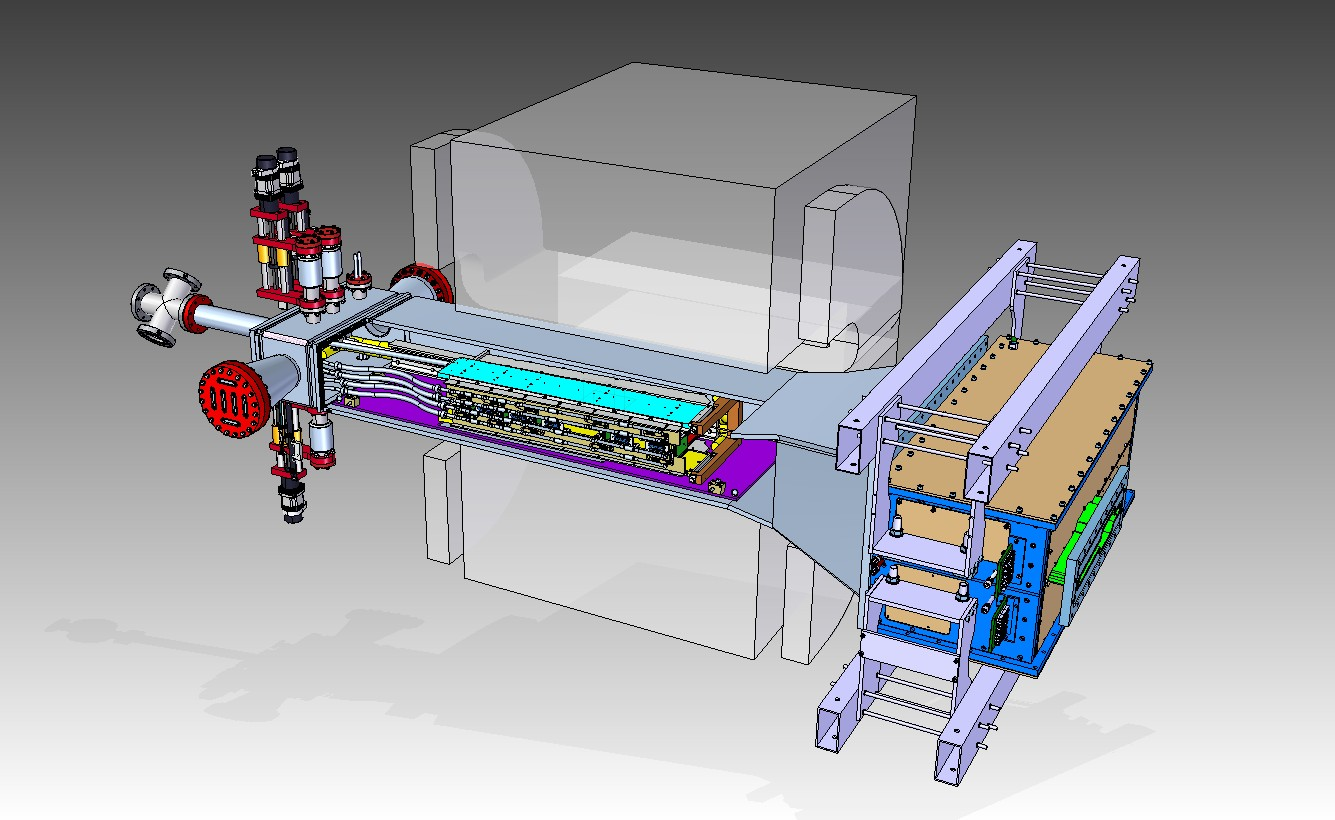
\includegraphics[width=0.8\textwidth]{figures/hps_testrun_rendering}
\caption{Rendering of the HPS Test apparatus installed on the beam line.}
\label{fig:testrundetector}
\end{figure*}
}
\end{center}
The HPS Test apparatus was designed to run in Hall~B at JLab using the CEBAF electron beam, a 
499~MHz beam, at an energy of 2.2 and 6.6~GeV and currents between 200 and 600~nA.  
The overall design of the experiment follows from the kinematics of \Aprime{} production which 
typically results in final state particles within a few degrees of the incoming beam, especially at low 
$m_{\textrm{A}^\prime}$. Detectors must therefore be placed close to the beam. 
The intense electron beam and the degraded electrons after the target are spread out horizontally by 
the analyzing magnet constitute a "dead zone" which must be completely avoided. The apparatus is 
split vertically $15$~mrad above and below the beam plane and the beam is transported in vacuum 
to minimize beam-gas interaction backgrounds. Even so, background occupancy in the detectors 
remain high and are dominated by the degraded primary beam, so high rate detectors, a fast trigger, 
and excellent time tagging are required to minimize their impact.  
At masses below $2 m_\mu$ only decays to electrons are allowed, so the key trigger comes from a PbWO$_{4}$ crystal calorimeter. 
 %\begin{multicols}{2}
\begin{center}
\begin{table*}[t]
{\small
\caption{Overview of the coverage, segmentation and performance of the HPS Test detector. }
\begin{tabular}{lccccccc}
\hline 
System & Coverage & \# channels & ADC & Time resolution & \# layers & Segmentation & Performance \\
 & (mrad) &  & (bit) & (ns) &  &  &  \\
\hline
SVT & $15<\theta_{y} < XXXX$ & 12800 & 14 & $\approx 2$~ns & 5  & $\approx 120~\mu$m $r-\phi$ & $\sigma_{d0,y}  \approx 100~\mu$m \\
& &  &  &  & (stereo layers) & $\approx 6~\mu$m $z$ & $\sigma_{d0,x} \approx 300~\mu$m \\
& &  &  &  &  &  & $\sigma_{d0,z}\approx 1$~mm \\
\hline
ECal & $15<\theta_{y} < XXXX$ & 442 & 12 & 4~ns & 1 & $1.3\times1.3$~cm$^2$  & $\sigma(E)/E \approx 4.5\%$ \\ 
 &  &  &  &  &  & $1.6\times1.6$~cm$^2$  &  \\ 
\hline
\end{tabular}
\label{tab:detector-overview}
}
\end{table*}
\end{center}
%\end{multicols}
A rendering of the HPS Test apparatus installed on the beam line is shown in 
Fig.~\ref{fig:testrundetector} and an overview of the coverage, segmentation and performance is 
given in Tab.~\ref{tab:detector-overview}.  

The silicon tracking and vertexing detector for HPS Test, or SVT, operates in an existing vacuum 
chamber inside the pair spectrometer analyzing magnet in Hall B at JLab.  There are five 
measurement stations, or ``layers,'' placed immediately downstream of the target. Each layer 
comprises a pair of closely-spaced silicon microstrip sensors responsible for measuring a single 
coordinate, or ``view.'' Introduction of a small (50 or 100~mrad) stereo angle between the two 
sensors of each layer provides three-dimensional tracking and vertexing throughout the acceptance 
of the detector with one redundant layer. Each layer In order to accommodate the dead zone, the 
SVT is built in two halves that are mirror reflections of one another about the plane of the nominal 
electron beam.  Each layer in one half are supported on a common support plate with independent 
cooling and readout. 

Each half of the electromagnetic calorimeter, or ECal, consists of 221 PbWO$_4$ crystals arranged 
in rectangular formation. There are five rows with 46 modules in each row except the row closest to 
the beam plane which has 37. The light from each crystal 
is read out by Avalanche Photodiode (APD) glued on the back surface of the crystal. 
Signals from the APDs were amplified using custom-made amplifier boards before being sent to the 
readout electronics.  

The  Data Acquisition system combines two architectures, the Advanced Telecom Communications 
Architecture (ATCA) based SVT readout system and VXS based digitization and triggering system for 
the ECal. The system was designed to run at up to 20~kHz trigger rate.


%%%%%%%%%%%%%%%%%%%%%%%%%%%%%%%%%%%%%%%%%%%%%%%%%%


\section{The HPS Test Run Beamline}
The HPS Test run studied multiple Coulomb scattering of electrons and positrons from 
bremsstrahlung photons produced in the Hall B tagged photon facility. 
Figure~\ref{fig:hpstest_layout} shows the layout of 
the HPS Test setup on the beam line. The SVT was installed inside the Hall B pair 
spectrometer magnet (PS) vacuum chamber with the ECal mounted downstream of it. Both the 
SVT and the ECal were retracted off the beam plane compared to nominal electron beam runing to 
allow clean passage of the photon beam through the system. 
\begin{figure}[ht]
    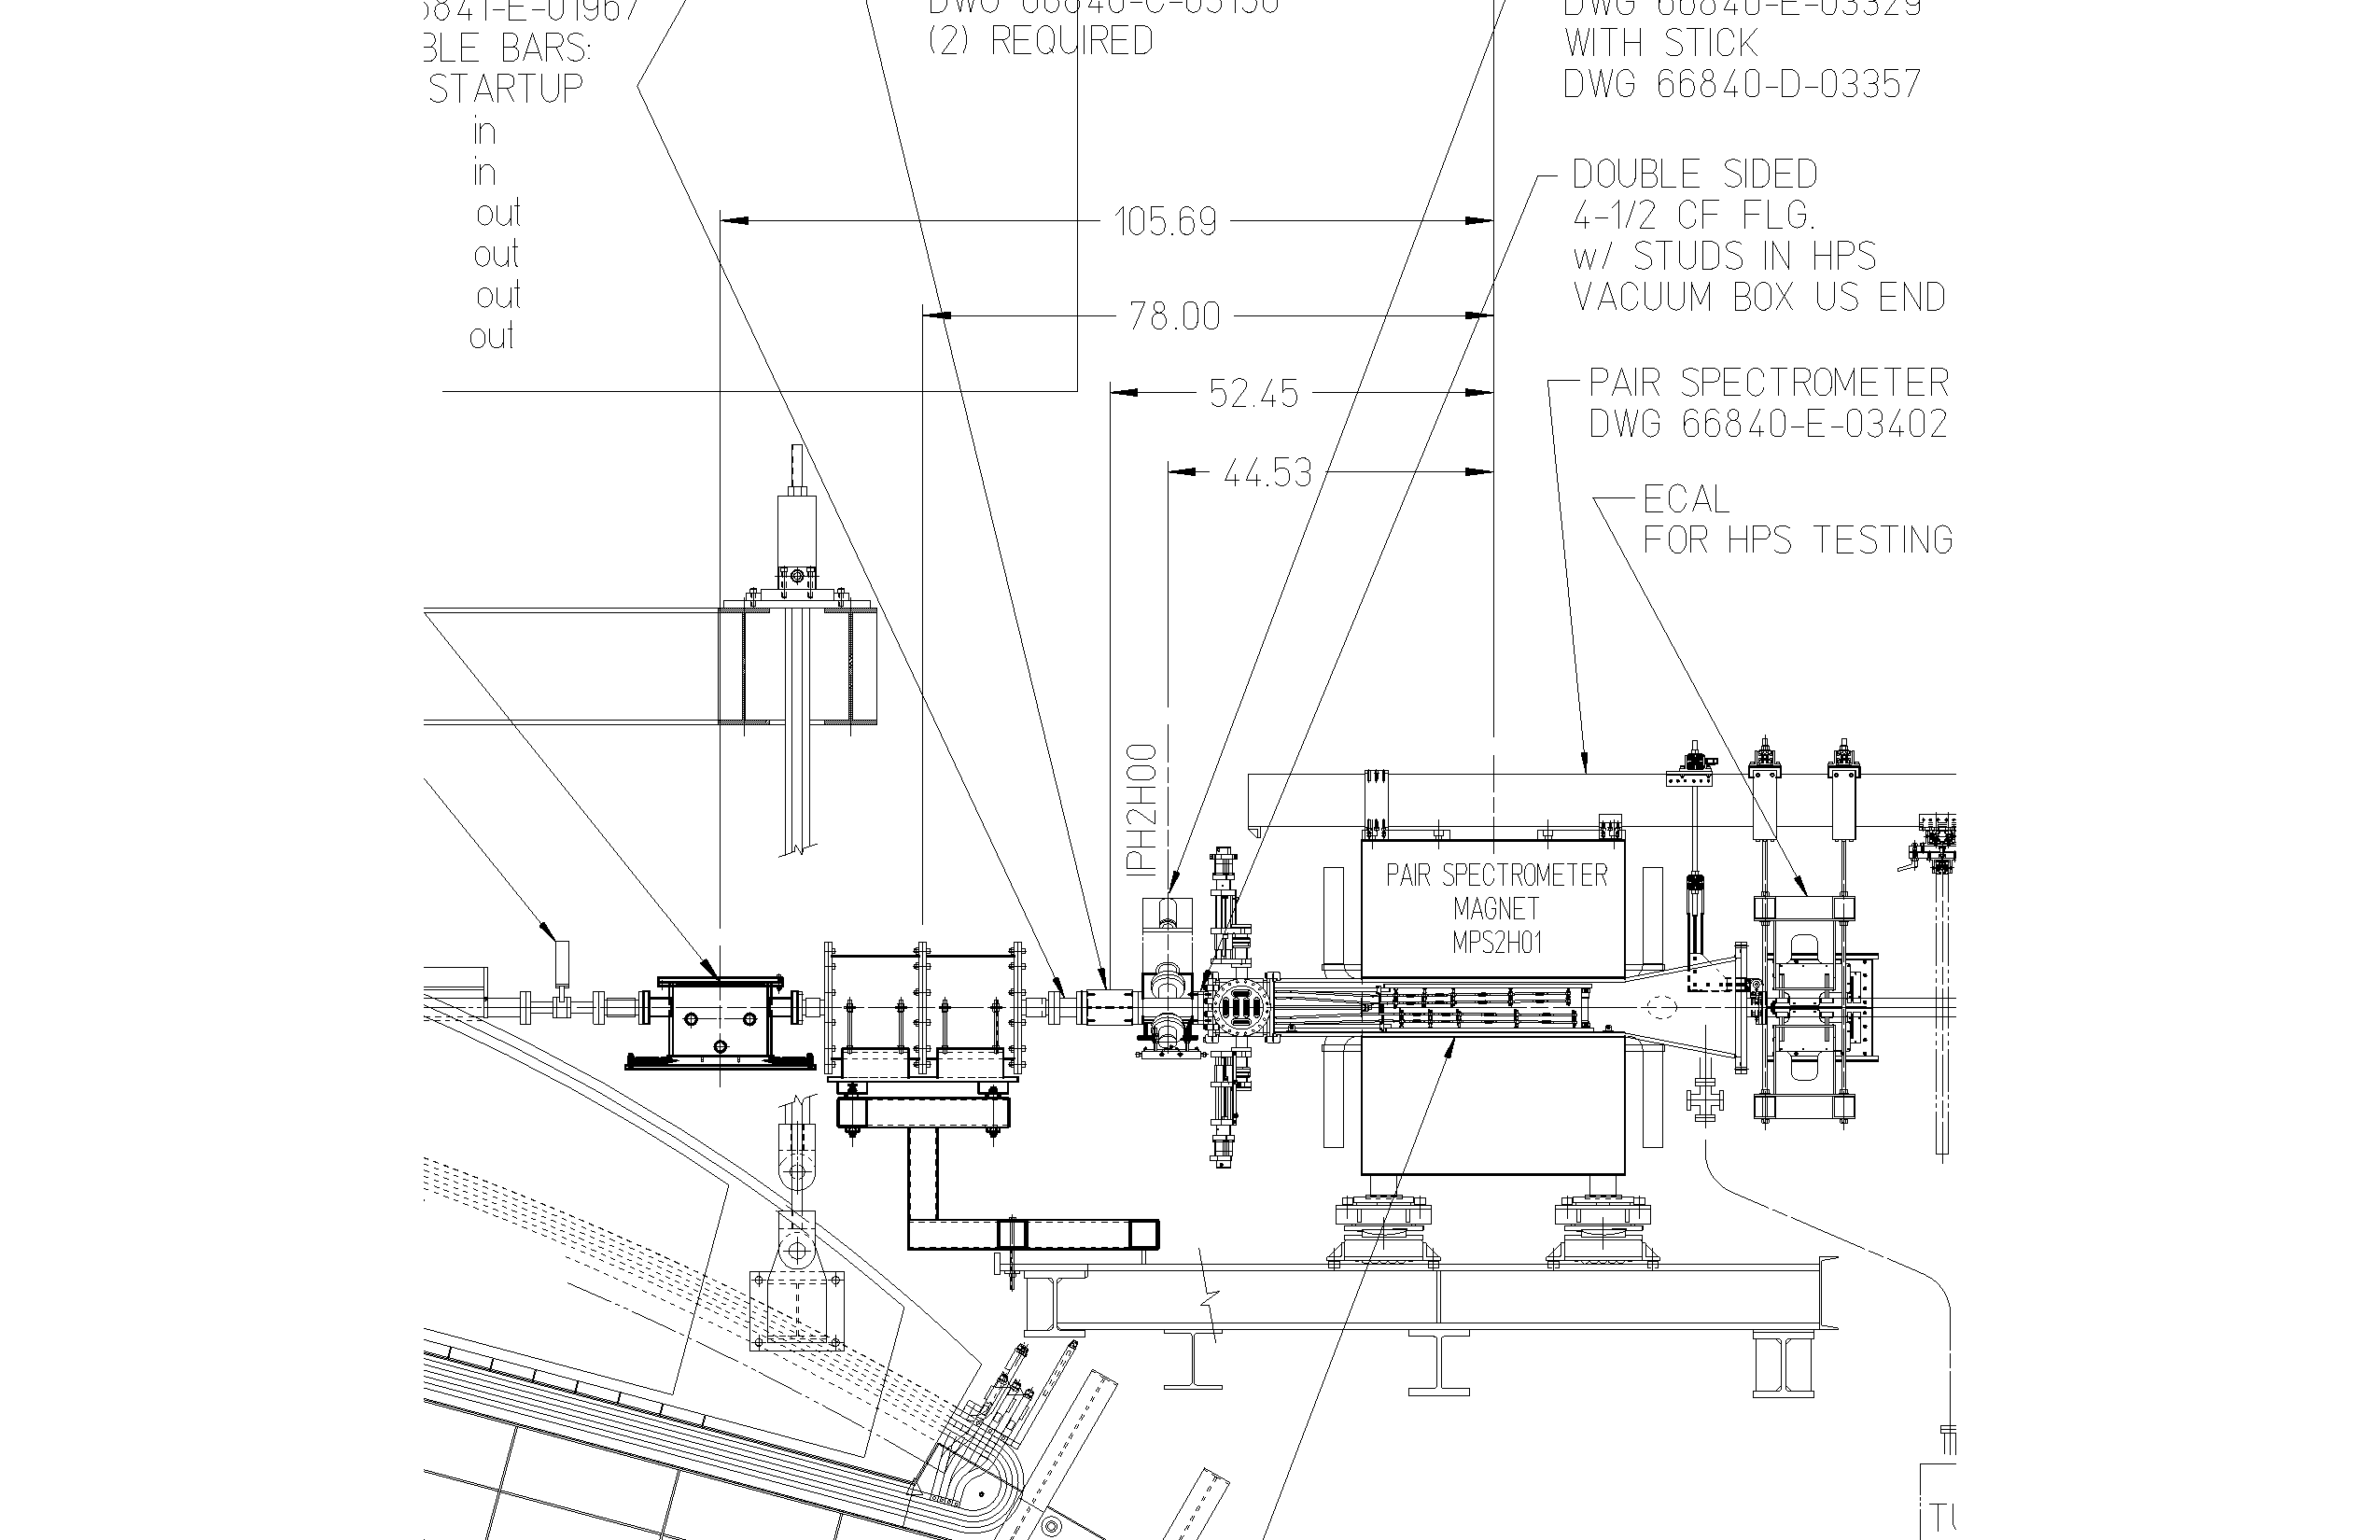
\includegraphics[width=0.5\textwidth]{figures/HPS_dimensions}
\caption{\small{Layout of the HPS parasitic run.} }
\label{fig:hpstest_layout}
\end{figure}

The photon beam was generated in the interaction of $5.5$~GeV electrons with a $10^{-4}~X_0$ 
gold radiator located $\approx~9$~m upstream of the PS. The primary beam and scattered 
electrons are deflected away from detectors by the dipole magnet of the photon tagging system. 
During the dedicated HPS Test run period, the collimated (6.4~mm diameter), photon beam passes 
through the aluminum PS pair converter and later the HPS system as shown schematically in Fig.~\ref{fig:schematic_testrun_vs_erun}.
\begin{figure}[ht]
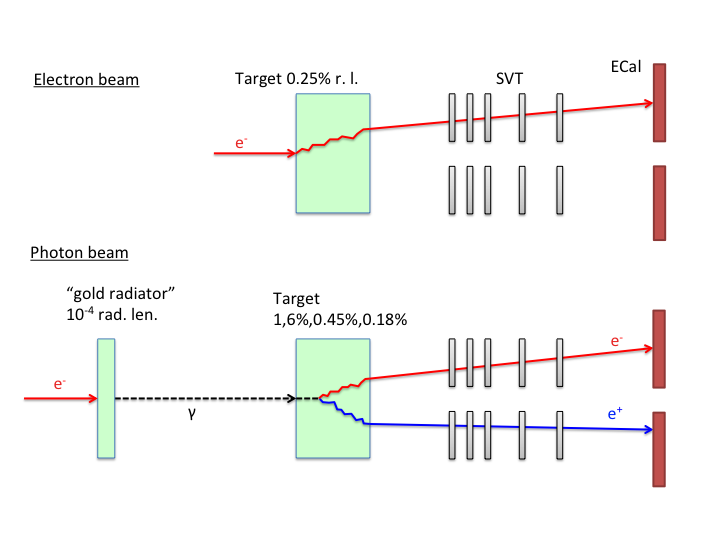
\includegraphics[ width=7cm]{figures/photon_vs_electron_beam_schematic.png}
\caption{\small{Schematic comparison of HPS Test run photon beam compared to the HPS electron beam.}}\label{fig:schematic_testrun_vs_erun}
\end{figure}
The PS pair converter was located $\approx~77$~cm upstream of the first layer of the SVT.
Data was taken on different converters (empty, $1.8\times 10^{-3}~X_0$ , $4.5\times 10^{-3}~X_0$ 
and $1.6 \times 10^{-2}~X_0$) and repeated with the reverse field setting of the PS dipole magnet.




%%%%%%%%%%%%%%%%%%%%%%%%%%%%%%%%%%%%%%%%%%%%%%%%%%

\section{Silicon Vertex Tracker}
\label{svt}

The Silicon Vertex Tracker (SVT) enables efficient reconstruction of charged particles and precision 
determination of their trajectories. These measurements allow \Aprime{} decays to be distinguished 
from background via simultaneous estimation of the invariant mass of \ee{} decay products and the 
position of decay vertexes downstream of the target. 

%Track reconstruction is also important for energy scale calibration of the electromagnetic calorimeter due to the better momentum resolution of tracks compared to clusters in the calorimeter.

%\subsection{SVT Requirements and Constraints}
%The primary goal was to demonstrate that the technology and design approach 
%chosen for the SVT was sound for running in the challenging environment at JLab. 
%Nevertheless, a secondary but 
%important aspect was that, after proving the technical concepts,  the apparatus would have the 
%capability to discover \Aprime{} events. The implication was that the design of the SVT in the 
%HPS Test apparatus would be subject to almost the same constraints and requirements as the full 
%experiment except for certain aspects regarding longevity and robustness subject to cost, beam time 
%and construction and design time constraints for the Test run. 

The design of the SVT is primarily driven by direct physics requirement and constraints from the 
environment at the interaction region. The \Aprime decay products 
have momenta in the range of 1~GeV, so multiple scattering dominates mass and vertexing 
uncertainties for any possible material budget, so the SVT must minimize the amount of 
material in the tracking volume. The signal yield for long-lived \Aprime's is very small, so 
the rejection of prompt vertexes must be exceedingly pure, on the order of $10^{-7}$, in order to 
eliminate all prompt backgrounds. To achieve the required vertexing performance the first layer of the 
SVT must be placed no more than about 10 cm downstream of the target. At that distance, it is found 
that the active region of a sensor can be placed as close to 1.5 mm from the center of the beam, 
defining the 15 mrad ``dead zone" mentioned previously, to maximize low-mass \Aprime acceptance 
with decay products nearly collinear with the beam axis. At the edge of this ``dead zone," the 
radiation dose approaches $10^{15}$ electrons/cm$^2$/month, or roughly 
$3 \times 10^{14}$~\fluenceunit{}/month~\cite{Rashevskaya:2002nd}, as shown in 
Fig.~\ref{fig:radiation},  requiring the sensors to be actively cooled.
% and~\ref{fig:rates}.
%===================
\begin{figure}[]
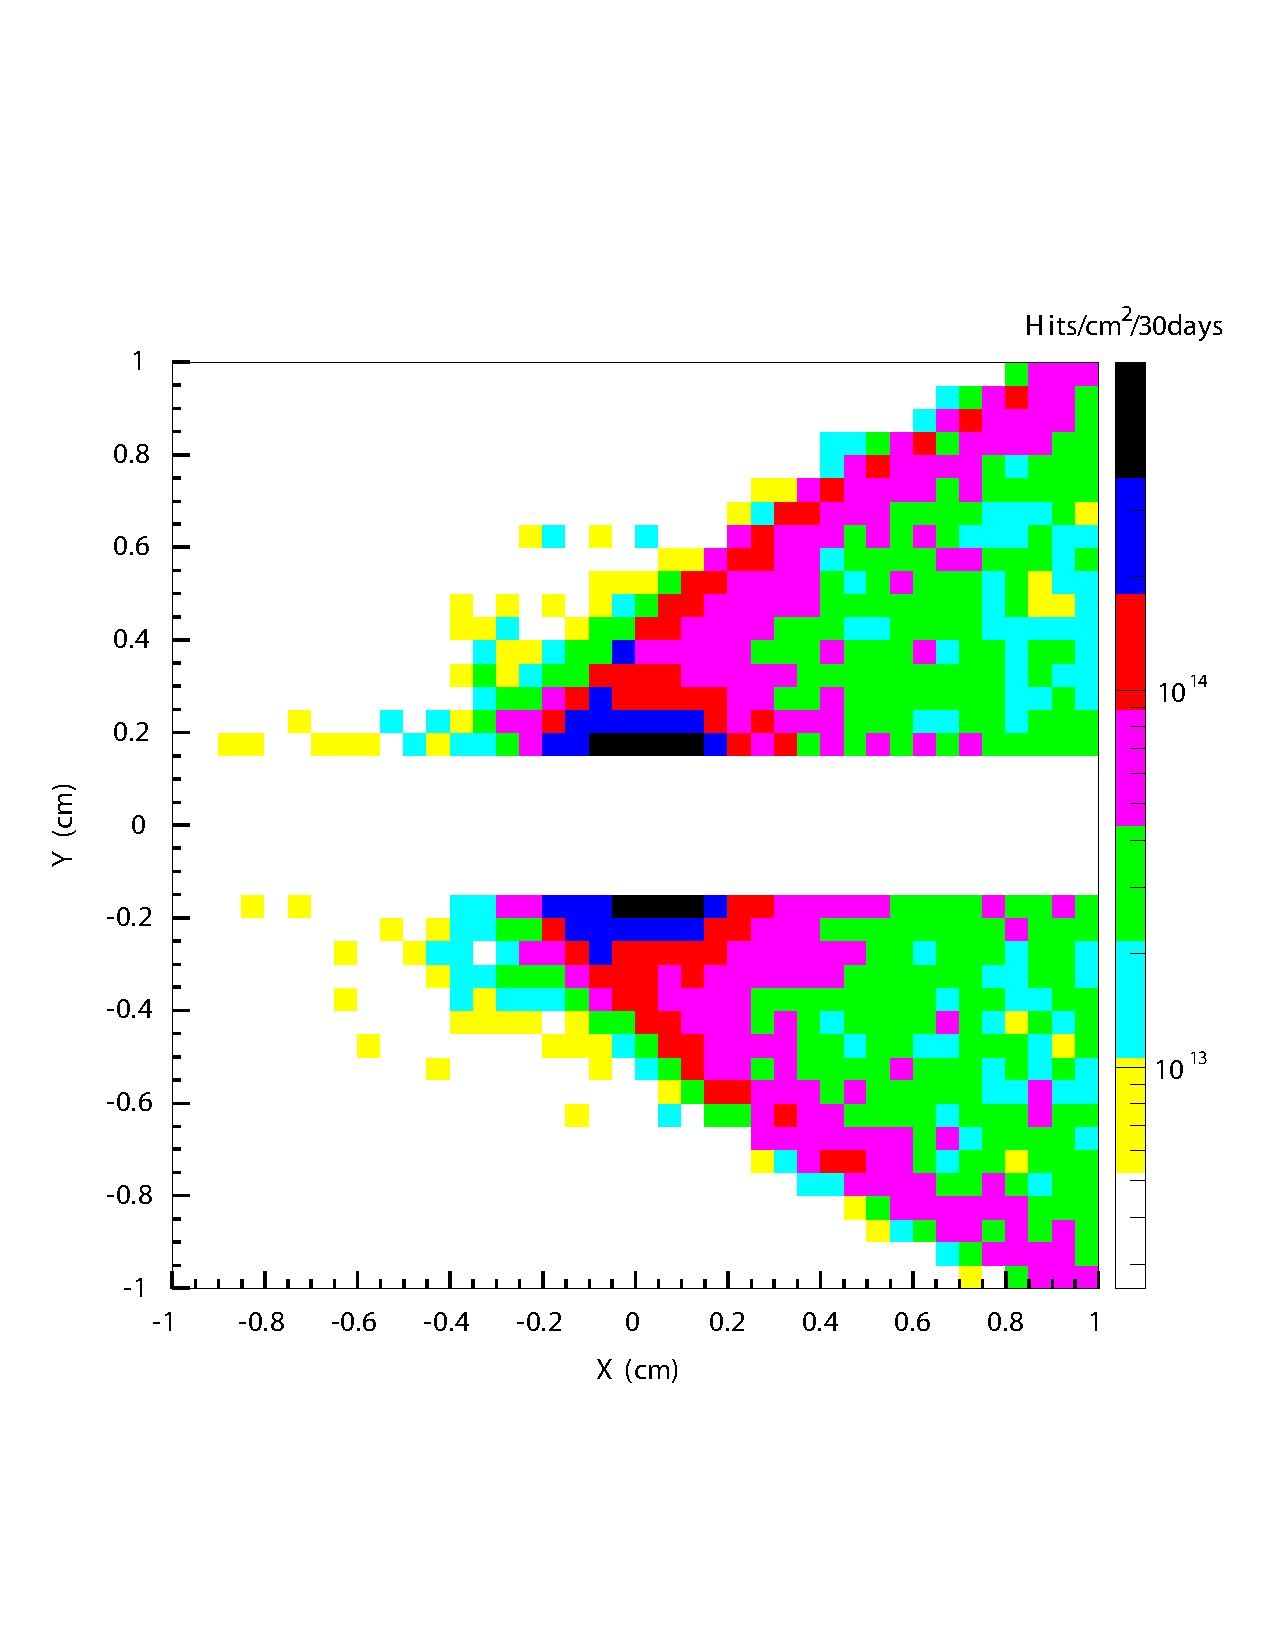
\includegraphics[width=7cm]{figures/radiation}
\label{fig:radiation}
\caption{{\small Simulation of the electron fluence 10~cm downstream of the target in the active region 
of the SVT ($|Y|>0.15~$mm) looking downstream; electrons bend towards $+x$.}}
\end{figure}
Meanwhile, very low-energy delta rays from 
beam-gas interactions multiply the density of background hits, so the SVT must operate inside the 
beam vacuum.  Finally, in order to protect the sensors, the detector must be movable so that it can be 
retracted during periods of uncertain beam conditions.  



\subsection{Layout}
The layout of the SVT is summarized in Tab.~\ref{tab:trk} and rendered in Fig.~\ref{fig:tracker_model}. 
Each of the layers is comprised of a pair of closely-spaced silicon microstrip sensors mounted back-
to-back to form a module. A 100~mrad stereo angle is used in the first three layers to provide higher-
resolution 3D space points for vertexing.  Using 50~mrad in the last two layers breaks the tracking 
degeneracy of having five identical layers and minimizes fakes from ghost hits to improve pattern 
recognition. Altogether, the SVTcomprises 20 sensors for a total of 12780 readout channels. 
%=======================
\begin{center}
\begin{table}[ht]
{\footnotesize
\begin{tabular}{lccccc}   
\hline \hline 
    Layer & 1 & 2 & 3 & 4 & 5 \\      
\hline
    $z$ from target (cm)  & 10 & 20 & 30 & 50 & 70  \\ 
    Stereo angle (mrad)  & 100 & 100 & 100 & 50 & 50 \\ 
    Bend res. ($\mu$m)  & $\approx$60 & $\approx$60 & $\approx$60 & $\approx$120 & $\approx$120  \\ 
    Non-bend res. ($\mu$m)  & $\approx$6 & $\approx$6 & $\approx$6 & $\approx$6 & $\approx$6  \\ 
    \# of sensors  & 4 & 4 & 4 & 4 & 4  \\ 
    Dead zone (mm) & $\pm1.5$  & $\pm3.0$  & $\pm4.5$  & $\pm7.5$  & $\pm10.5$  \\ 
    Power cons. (W) & 6.9 & 6.9 & 6.9 & 6.9 & 6.9 \\
\hline \hline
\end{tabular}
\caption{\small Layout of the SVT.}
}
\label{tab:trk}
\vspace*{-15mm}
\end{table}
\end{center}
%=======================
\begin{center}
\begin{figure}[htp]
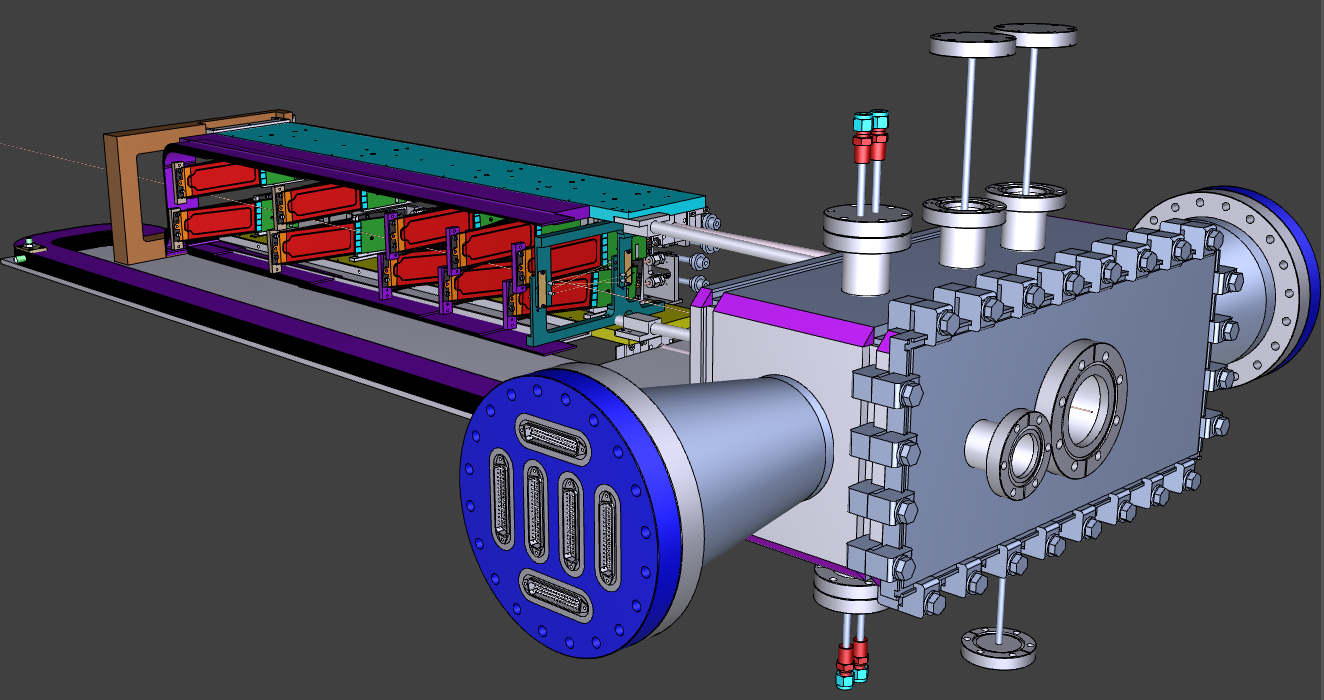
\includegraphics[width=7cm]{figures/HPS_nochamber}
\caption{\small A rendering of the SVT showing the modules on their support plates held by the 
hinged C-support on the left and the motion levers on the right. The sensors are shown in red and the 
hybrid readout boards in green. The beam enters from the right through a vacuum box with flanges 
for services. }
\label{fig:tracker_model}
%\vspace*{-5mm}
\end{figure}
\end{center}
%=======================
The SVT is built in two separate halves that are mirror reflections of one another about the plane of 
the nominal electron beam.  Each half consists of five modules mounted on a support plate that 
provides services to the modules and allows them to be moved as a group relative to the dead zone. 
The two halves of the tracker are connected to hinges mounted on a C-shaped support just beyond 
the last layer that defines the nominal spacing between the upper and lower halves of the tracker.  A 
shaft attached to each support plate in front of layer 1 extends upstream and connects to a linear shift 
that transfers motion into the vacuum box through bellows to open and close the two halves around 
the dead zone. The C-support is mounted to an aluminum baseplate that defines the position of the 
SVT with respect to the vacuum chamber. Figure~\ref{fig:tracker_halves} shows a photograph of both 
completed detector halves prior to final assembly. 
%=======================
\begin{figure}[htp]
\begin{center}
    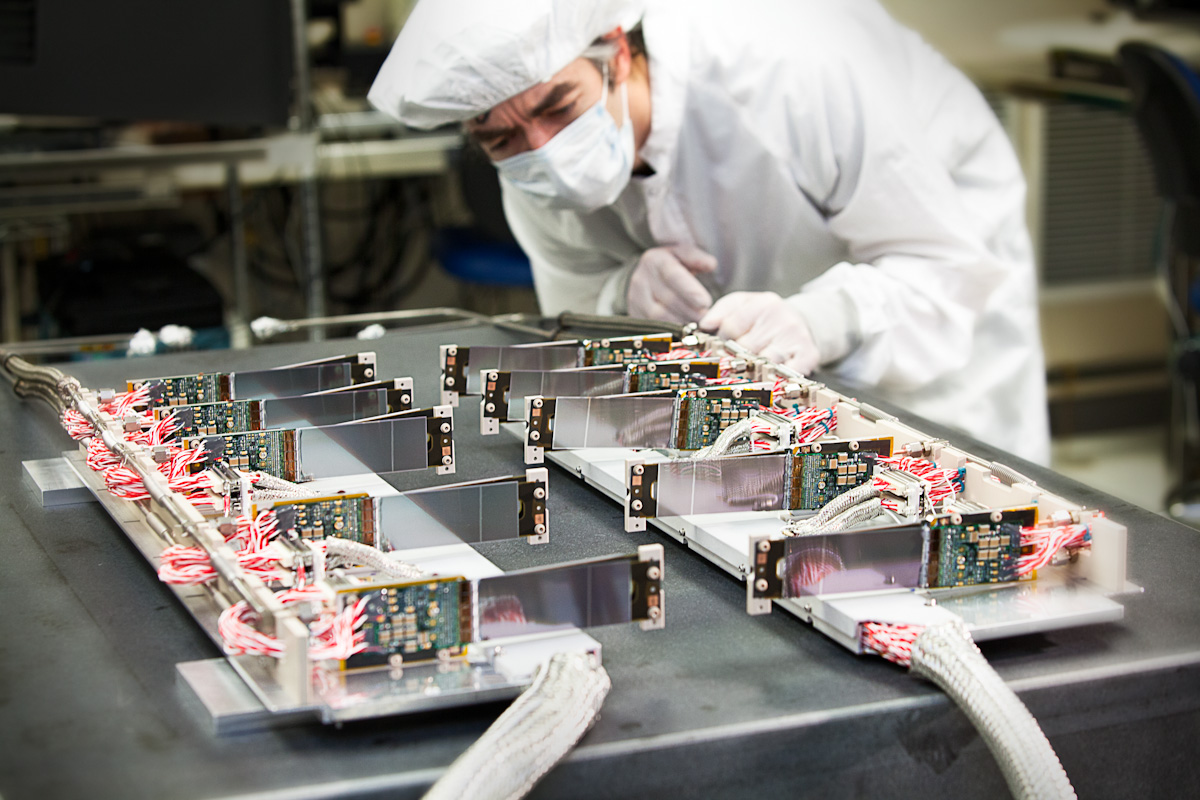
\includegraphics[width=7cm]{figures/2012-101-PHOTON-DETECTOR-001}
\caption{\small{Both halves of the HPS Test SVT after final assembly at SLAC.  The cooling manifolds and 
integrated cable runs are clearly seen.} }
\label{fig:tracker_halves}
\end{center}
%\vspace*{-5mm}
\end{figure}
%=======================

\subsection{Components}
The sensors for the SVT are $p+$-on-$n$, single sided, AC coupled, polysilicon-biased microstrip 
sensors fabricated on $<100>$ silicon and have 30 (60) micron sense (readout) pitch over their 
$4\times10$~cm$^2$ surface. This sensor technology was selected to match the requirement of 
a $<1$\% $X_0$ per layer, single-hit resolution better than 50~$\mu$m and tolerant of a radiation 
dose of approximately $1.5\times10^{14}$~\fluenceunit{} for a six month run. The sensors 
were purchased from the Hamamatsu Photonics Corporation for the cancelled 
Run 2b upgrade of the D\O~experiment~\cite{Denisov:2001aa} which satisfied the requirement that 
the technology must be mature and available within the time and budget constraints.

%\subsubsection{Front-end Electronics}
Despite having only small spots with very high occupancy (up to 4~MHz/mm$^2$) closest to the primary 
beam, see Fig.~\ref{fig:radiation}, the rates are still high and lowering the peak occupancy to 
approximately 1\% for tracking requires a trigger window and hit time tagging of roughly 8~ns. The 
ECal readout and trigger described in Sec.~\ref{sec:fadc} can achieve such resolution. To reach this 
performance the sensors for the SVT are readout by the APV25 ASIC developed for the CMS 
experiment at CERN~\cite{French:2001xb}. The APV25 can capture two successive samples of three 
of the output of the shaper at a sampling rate of approximately 40~MHz.  By fitting the known 
$CR$-$RC$ shaping curve to these samples, the initial time of the hit can be determined to a precision 
of 2~ns for S/N$\approx25$~\cite{Friedl:2009zz}.  For electron beam running, six-sample readout and 
the shortest possible shaping time (35~ns) is used to best distinguish hits that overlap in time.
The APV25 ASICs are hosted on simple FR4 hybrid readout boards, outside the tracking volume, with a 
short twisted-pair pigtail cable to provide power and configuration and signal readout. Along with a 
single sensor, these are glued to a polyamide-laminated carbon fiber composite backing making 
up a half-module. A window is machined in the carbon fiber leaving only a frame around the periphery 
of the silicon to minimize material. A 50~$\mu$m sheet of polyamide is laminated to the surface of the 
carbon fiber with 1~mm overhang at all openings to ensure good isolation between the backside of the 
sensor, carrying high-voltage bias, and the carbon fiber which is held near ground. 

The sensor modules for the SVT consist of a pair of identical half-modules, sandwiched back-to-back 
around an aluminum cooling block at one end and a similar PEEK spacer block at the other. 
Figure~\ref{fig:tracker_module} shows a single module after assembly.
%=======================
\begin{figure}[htp]
	\begin{center}
   	 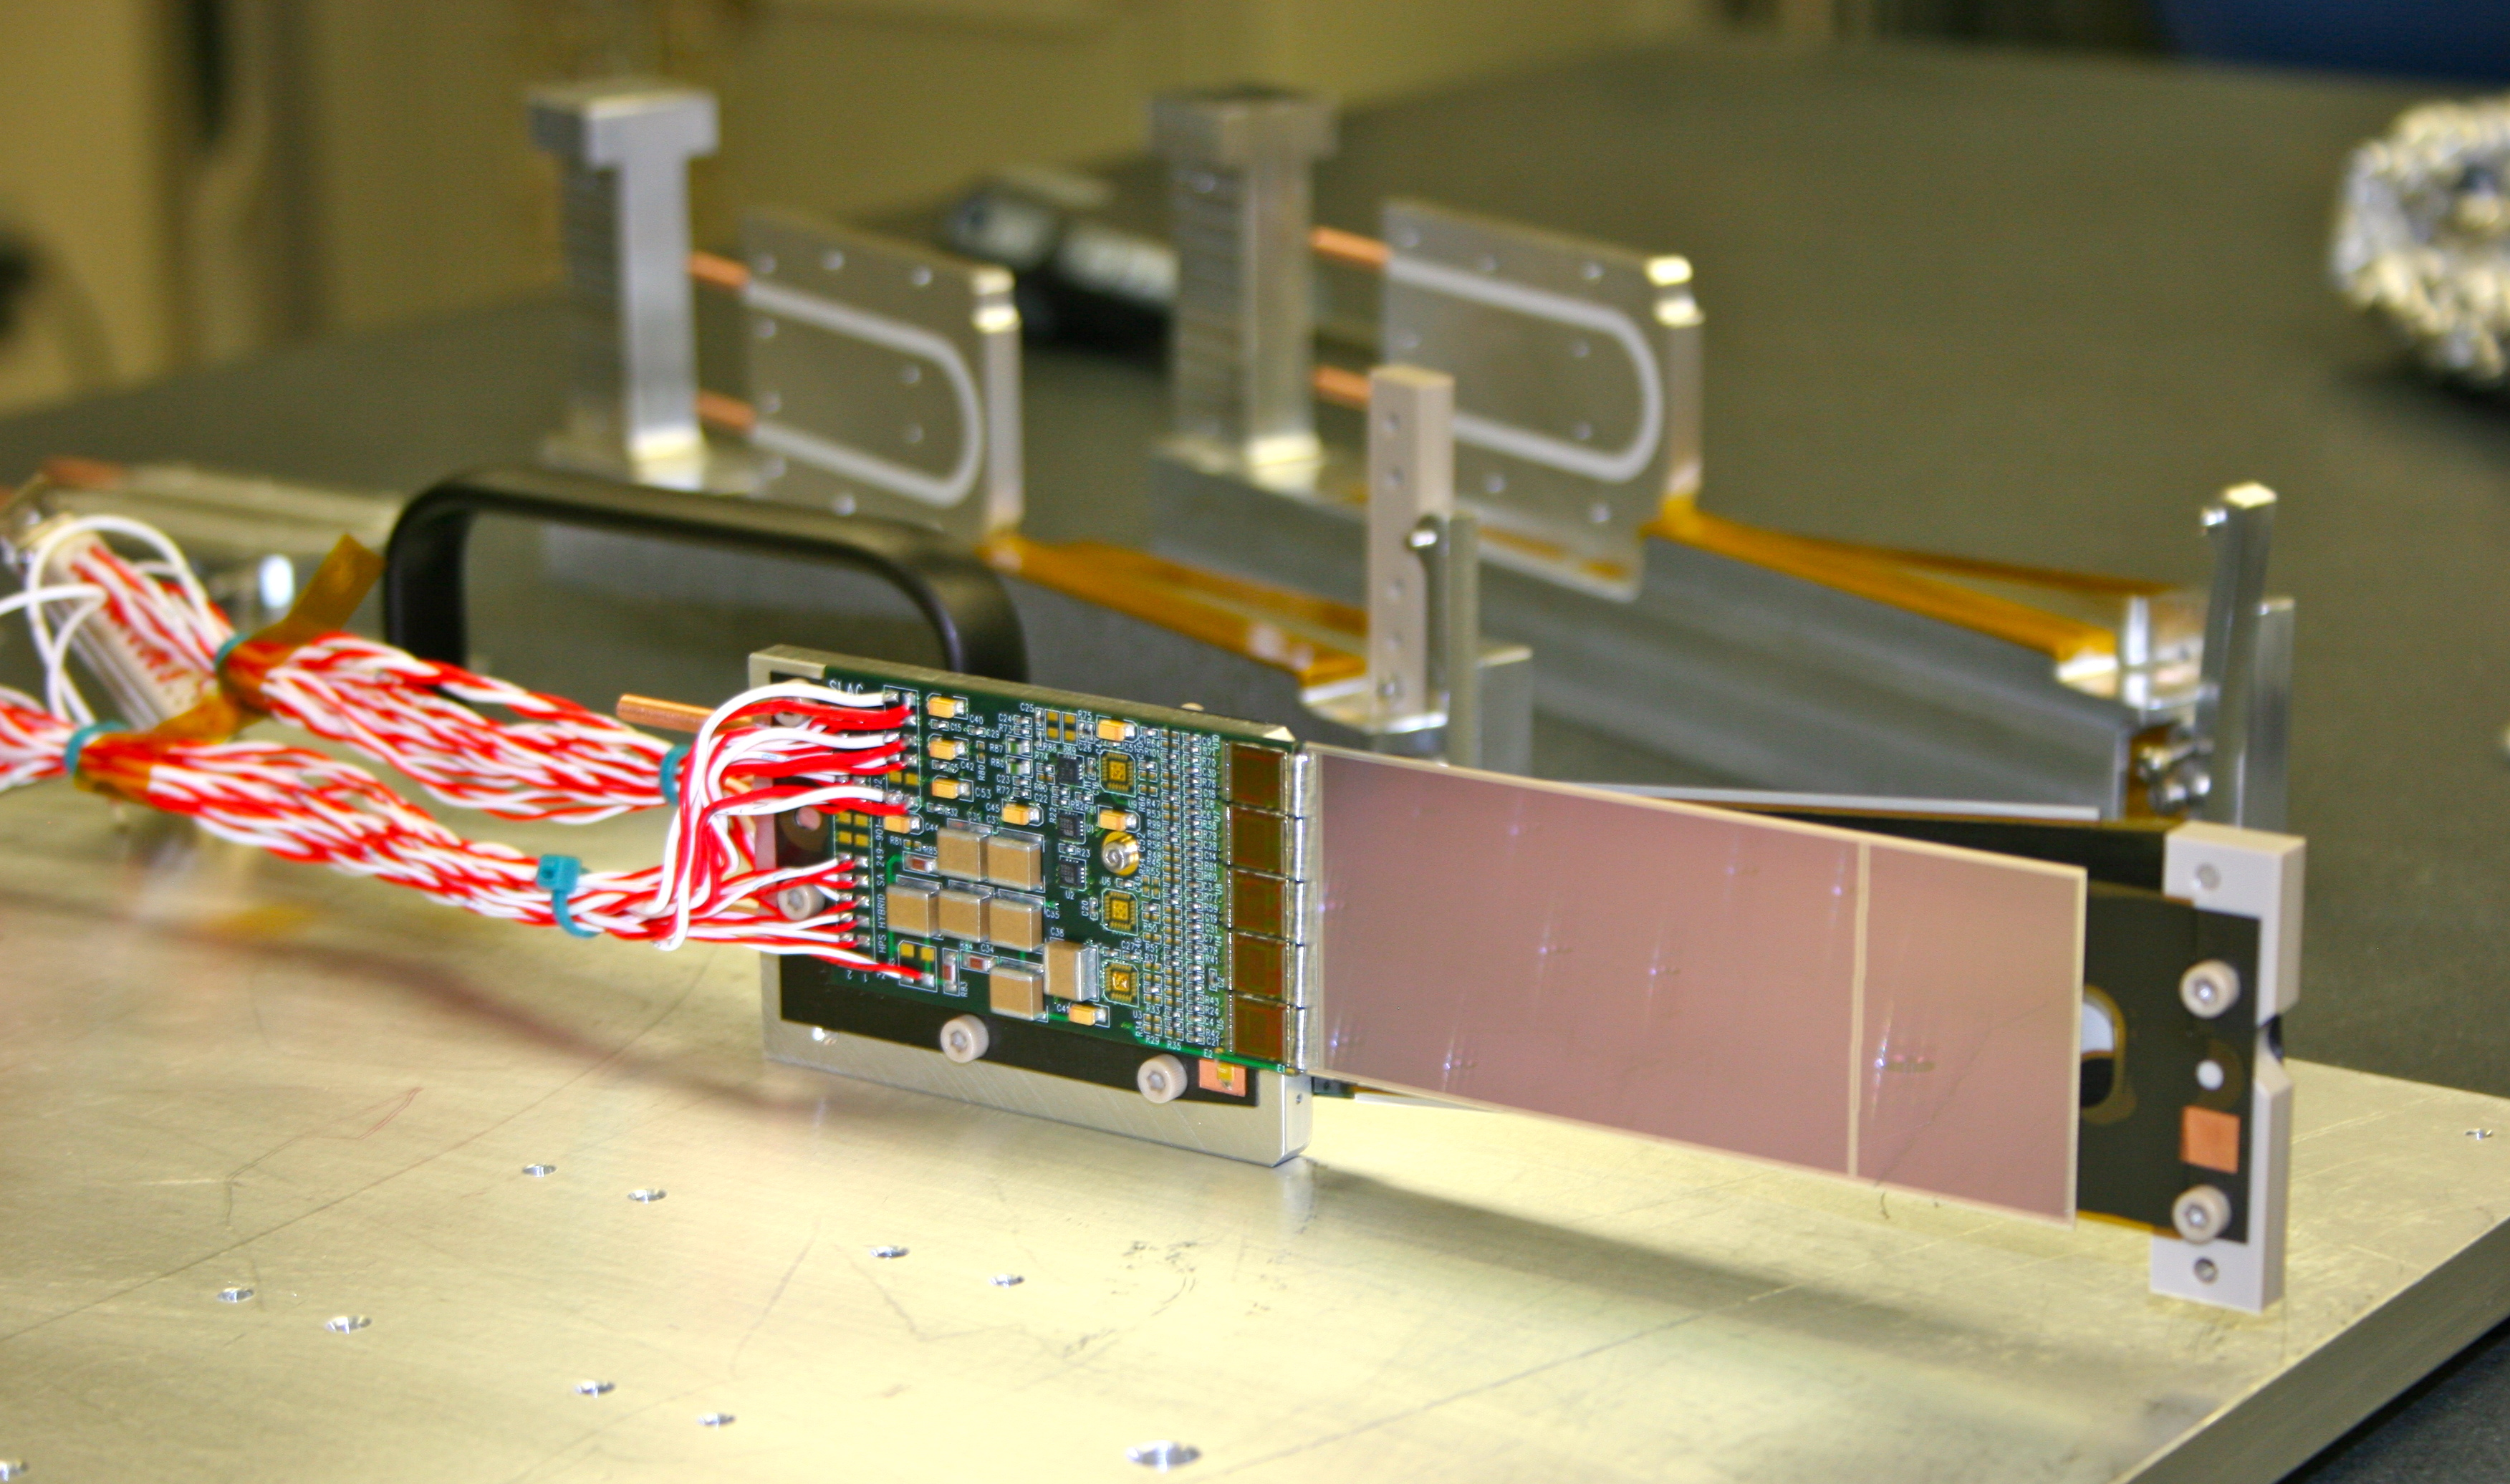
\includegraphics[width=7cm]{figures/IMG_5200}
	\caption{\small{A prototype module assembly (foreground) with the 50~mrad (left) and 100~mrad (right) module assembly fixtures in the background.  A pair of cooling blocks and a spacer block can be seen on the fixtures.} }
	\label{fig:tracker_module}
	\end{center}
\vspace*{-5mm}
\end{figure}
%=======================
The cooling block provides the primary mechanical support for the module as well as cooling via copper 
tubes pressed into grooves in the plates. The spacer block defines the spacing between the sensors at 
the far end of the module, stiffens the module structure, and improves the stability of the sensor 
alignment.  The average support material in the tracking volume is approximately 0.06\% $X_{0}$ per 
double-sided module for a total material budget of 0.7\% per layer.

The total SVT power consumption budget of about 50~W is removed by a water/glycol mixture 
circulated through a flexible manifold attached to the copper tubes in the cooling blocks. During the Test 
run the sensors where operated at around $23^{\circ}$C. The power consumption is dominated by five 
APV25 ASICs on each hybrid board consuming approximately 2~W, radiant heat load is less than 
0.5~W per sensor and leakage current is only significant in a small spot after irradiation.  





\subsection{Digitization, Event Building and Data Transmission}
\label{sec:svt_daq}
The SVT data acquisition (DAQ) is based on the Reconfigurable Cluster Element (RCE) and cluster 
interconnect concept developed at SLAC as generic building blocks for DAQ systems. 
The RCE is a generic computational building block, housed on a separate daughter card called 
Data Processing Module (DPM), that are realized on an ATCA front board called the Cluster On Board 
(COB), see Fig.~\ref{fig:cob}.
 \begin{figure}[]
\begin{center}
{\small
	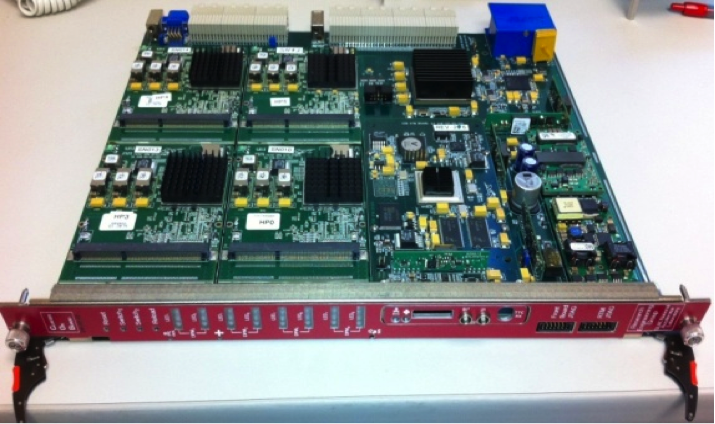
\includegraphics[width=6cm]{figures/svt_daq_module}
	\caption{The SVT DAQ COB board with four data processing daughter cards visible on the left side.}
	\label{fig:cob}
}
\end{center}
\end{figure}
The first generation RCE used in the Test run consisted of a Virtex~5 FPGA with 1~GB of DDR3 RAM. 
A schematic overview of the system is shown in Fig.~\ref{fig:svtdaq}. 
 \begin{figure}[]
\begin{center}
{\small
	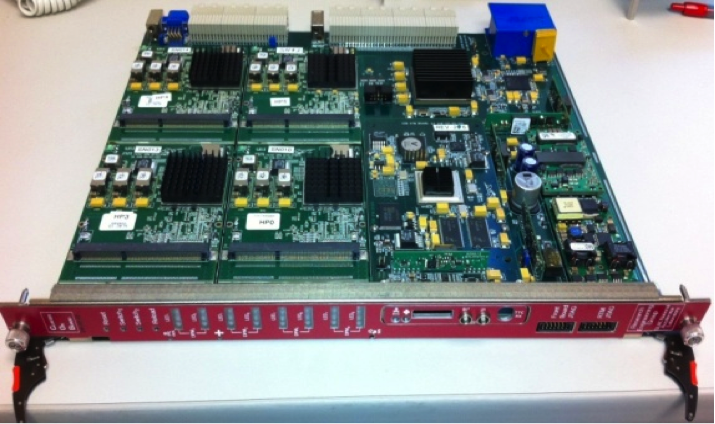
\includegraphics[width=6cm]{figures/svt_daq_module}
	\caption{Block diagram overview of the SVT DAQ.}
	\label{fig:svtdaq}
}
\end{center}
\end{figure}
The outputs of 12 SVT half-modules are digitized on the Rear-Transition-Module (RTM), a custom board 
on the back side of the ATCA crate, interfacing the HPS readout to the generic DAQ components on the 
COB. A pre-amplifier converts the APV25 differential current output to a different voltage output scaled to 
the sensitive range of a 14-bit ADC operating at the system clock of 41.667~MHz. The RTM is organized 
into four sections with each section supporting three SVT half-module hybrids (15 APV25 ASICs). The 
RTM also includes a 4-channel fiber optic module and supporting logic which is used to interface 
to the JLab trigger system supervisor. Each section of the RTM is input to a DPM which apply thresholds 
for data reduction and organizes the sample data into UDP datagrams. The DPM also hosts an I$^{2}$C 
controller used to configure and monitor the APV25 ASICs. A single ATCA crate with two COB cards 
was used, one supporting four DPMs and one supporting 3 DPMs and one DPM that is configured as 
the trigger and data transmission module. The two COB cards and their DPMs are interconnected with a 
10Gb/s switch card~\cite{Larsen:2011zb} which also hosts two 1Gb/s Ethernet interfaces to the external 
SVT DAQ PC.  

The external PC supports three network interfaces; two standard 1Gb/s Ethernet and one custom low 
latency data reception card. The first is used for slow control and monitoring of the 8 
DPM modules and the second serves as the interface to the JLAB data acquisition system. The third 
custom low latency network interface is used to receive data from the ATCA crate and supports a low 
latency, reliable TTL trigger acknowledge interface to the trigger DPM. This PC hosts the SVT control 
and monitoring software as well as the JLab Read Out Controller (ROC) application described in more 
detail in Sec.~\ref{sec:daq}.

While trigger rates during the Test run was significantly lower this system was tested at trigger rates up 
to 20~kHz and 50~MB/s.


\subsection{Production, Assembly and Shipping}

%Of the sensors tested during production, 90\% were capable of 1000~V bias voltage without breakdown. 
Hybrids with APV25 ASICs underwent quick qualification testing and each half-module was run at low 
temperature ($\approx5^{\circ}$ C) and fully characterized for pedestals, gains, noise and time response 
after assembly.  Of 29 half-modules built, 28 passed qualification testing, leaving 8 spare modules after 
completion of the SVT, all capable of 1000~V bias voltage without breakdown.  Full-module assembly 
and mechanical surveys were performed at SLAC before final assembly, testing and shipping of the 
SVT to JLab. A custom shipping container with nested crates and redundant isolation for shock and 
vibration was built in order to safely send the partly assembled SVT to JLab. At JLab, the entire SVT was 
integrated with the full DAQ and the power supplies before moving the module-loaded support plates to 
Hall B for final mechanical assembly and installation inside of the vacuum chamber.

\subsection{Alignment}
The SVT was aligned using a combination of optical, laser and touch probe surveys at SLAC and JLab. 
The optical survey of individual modules with precision of a few $\mu$m are combined with a 
touch-probe survey of the overall SVT support structure, with 25-100~$\mu$m precision, to locate the 
silicon sensor layers with respect to the support plates and the mechanical survey balls on the base 
plate. After full assembly and installation of the SVT at JLab, a mechanical survey of the SVT base plate 
position inside the pair spectrometer vacuum chamber is used to determine the global position of the 
SVT with respect to CEBAF beam line. The resulting survey-based alignment has the position of the 
silicon sensors correct to within a few hundred microns measured from tracks in the Test run data. 
A more sophisticated global track-based alignment technique to reach final alignment precision 
well below 50~$\mu$m is being developed.


%%%%%%%%%%%%%%%%%%%%%%%%%%%%%%%%%%%%%%%%%%%%%%%%%%


\section{Electromagnetic Calorimeter}
\label{sec:ecal}

The electromagnetic calorimeter, installed downstream of the tracker, performs two essential functions for the experiment: provides a trigger to DAQ system and 
is used in the analysis for electron identification. 
%The device is highly segmented. It is fast, able to readout at rates comparable to those in the tracker, and able to provide good spatial and energy information to the trigger electronics. Like the tracker, the electromagnetic calorimeter is split to avoid impinging on the �dead zone�. The beam and radiative secondaries pass between the two of the calorimeter in vacuum, to avoid generating unnecessary backgrounds.
%Step\subsection{Purpose and Design Requirements}
%StepThe electromagnetic calorimeter (ECal) provide the trigger for the data acquisition and will be used for electron identification during the data analysis. The ECal is positioned after the analyzing dipole magnet and cover the full acceptance region of the SVT. It consist of two halves, split in the horizontal beam plane. The gap between upper and lower parts, $XXXX$~mrad (15mrad for electron running),  as seen from the target location, is necessary to avoid the "dead zone" where occupancy and radiation prevents any instrumentation to be situated.  
The energy of electrons of interest in HPS experiment will be in the range 
$0.5-6.5$~GeV. The ECal modules must have sufficient radiation lengths to absorb the full energy of these 
scattered electrons, have fine enough granularity to handle a high rate of electromagnetic 
background and survive large doses of radiation, especially near the beam plane. In addition, it needs to 
have excellent hit time resolution, $<10$~ns, in order to beat down beam backgrounds.  

Requirements of a compact design, operation at high radiation and high rate environment, in the presence of a 
high magnetic field are fulfilled by a lead-tungstate (PbWO$_{4}$) crystal calorimeter with magnetic field 
resistant Avalanche Photodiode (APD) readout.  Such calorimeter has been operational in the inner 
part of the CLAS detector for experiments in Hall-B at JLab since 2005 and meet all requirements set by 
HPS. The modules from this calorimeter have been subsequently repurposed for the ECal. 


\subsection{Components}

%Step\subsubsection{PbWO$_4$ Crystals}
The HPS test run ECal uses PbWO$_{4}$ crystals, APDs, and preamplifier boards from the inner calorimeter (IC) of the CLAS detector\cite{2008erhm.conf..421N}.  In Figure~\ref{fig:ecal-module} a schematic view of the module assembly is shown. Lead-tungstate crystals are $160$ mm long and are tapered with front face of $13.3\times13.3$~mm$^2$, tapered to $16\times16$~mm$^2$ at the rear face. The crystals were fabricated with very tight tolerances: $19~\mu$m for 13.3~mm dimension and $13~\mu$m for the 16~mm dimension. Each crystal is wrapped in VM2000 multilayer polymer mirror film.
The APDs (Hamamatsu S8664-55) with $5\times5$~mm$^2$ active area and $75\%$ quantum efficiency were glued on the rear face of the crystals using MeltMount 1.7 thermal plastic adhesive. The low gain of APDs ($\sim 200$) was compensated with custom made preamplifier boards, which provide factor 2000 amplification of the ADP signal. 
\begin{figure}[]
\begin{center}
{\small
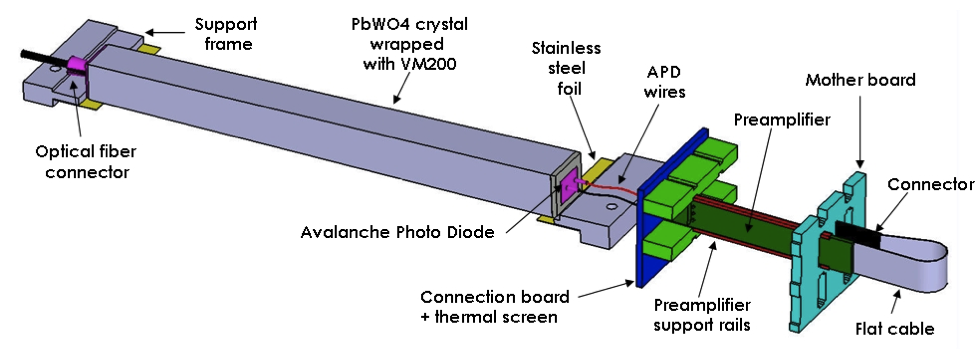
\includegraphics[width=7cm]{figures/ecal-module-schematic.png}
\caption{Schematic vied of an ECal module.}
\label{fig:ecal-module}
}
\end{center}
\end{figure}

\subsection{Layout}

Like the tracker, the electromagnetic calorimeter is split into two parts, beam-up and beam-down, to avoid impinging on the �dead zone�. The two parts of the Ecal are separated by a vacuum chamber, see Fig.~\ref{fig:ecal}. The beam and radiative secondaries pass between the two parts in vacuum, to avoid generating unnecessary backgrounds. The crystal modules in each part are arranged in rectangular formation, as shown in top panel of Fig.~\ref{fig:ecal}. There are 5 layers in each formation. Each layer has $46$ crystals except for the layers closest to the beam 
plane where 9 modules were removed to allow a larger opening for the outgoing electron and photon beams. 
In order to have stable light yield from crystals, and stable operation of APDs and preamplifiers, the module assembly of each ECal part was enclosed inside a temperature controlled box. 

Inside the box PbWO$_{4}$ crystals were supported by aluminum frames stacked on top of each other.  The bias voltage for APDs ($\sim 400$ V), the low voltage for preamplifiers ($\pm 5$ V), and the signals from APDs were transmitted in and out of the enclosure through a backplane called motherboard. The $221$ modules in each part of the ECal were divided into two low voltage groups and 12 bias voltage groups. Modules in bias voltage groups were selected to have gain uniformity of $\sim 20\%$.  

During the test run ECal was mounted downstream of the analyzing dipole magnet at the distance of about $147$~cm from the 
upstream edge of the magnet. 
%The two ECal modules are positioned just above and below the ECal vacuum chamber as shown in bottom panel of Fig.~\ref{fig:ecal}. 
%The primary electron beam, scattered electrons and bremsstrahlung photons pass through the system in vacuum. 
The gap between innermost edge of the crystals of two parts was $7.4$~cm, centered on the beam plane. The temperature stability of the system during the test run was better than $1^\circ~$F, the temperature uniformity inside the box was better than  $4^\circ~$F. 
\begin{center}
{\small
\begin{figure*}[htb]
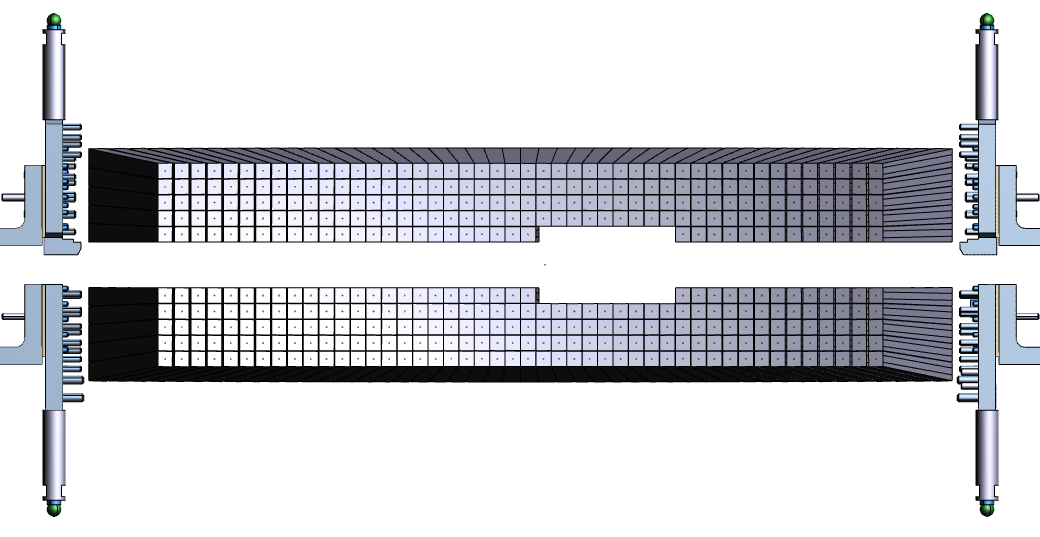
\includegraphics[width=0.45\textwidth]{figures/ECal}
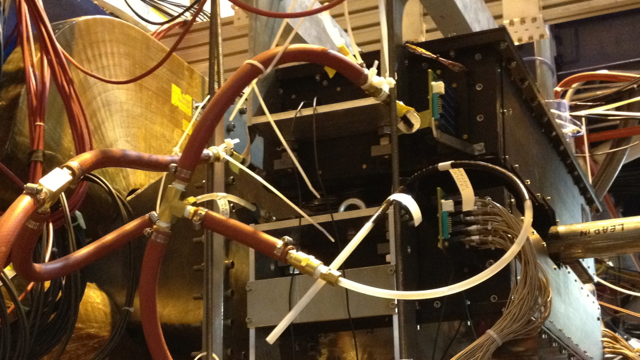
\includegraphics[width=0.45\textwidth]{figures/ecal_picture_beamline}
%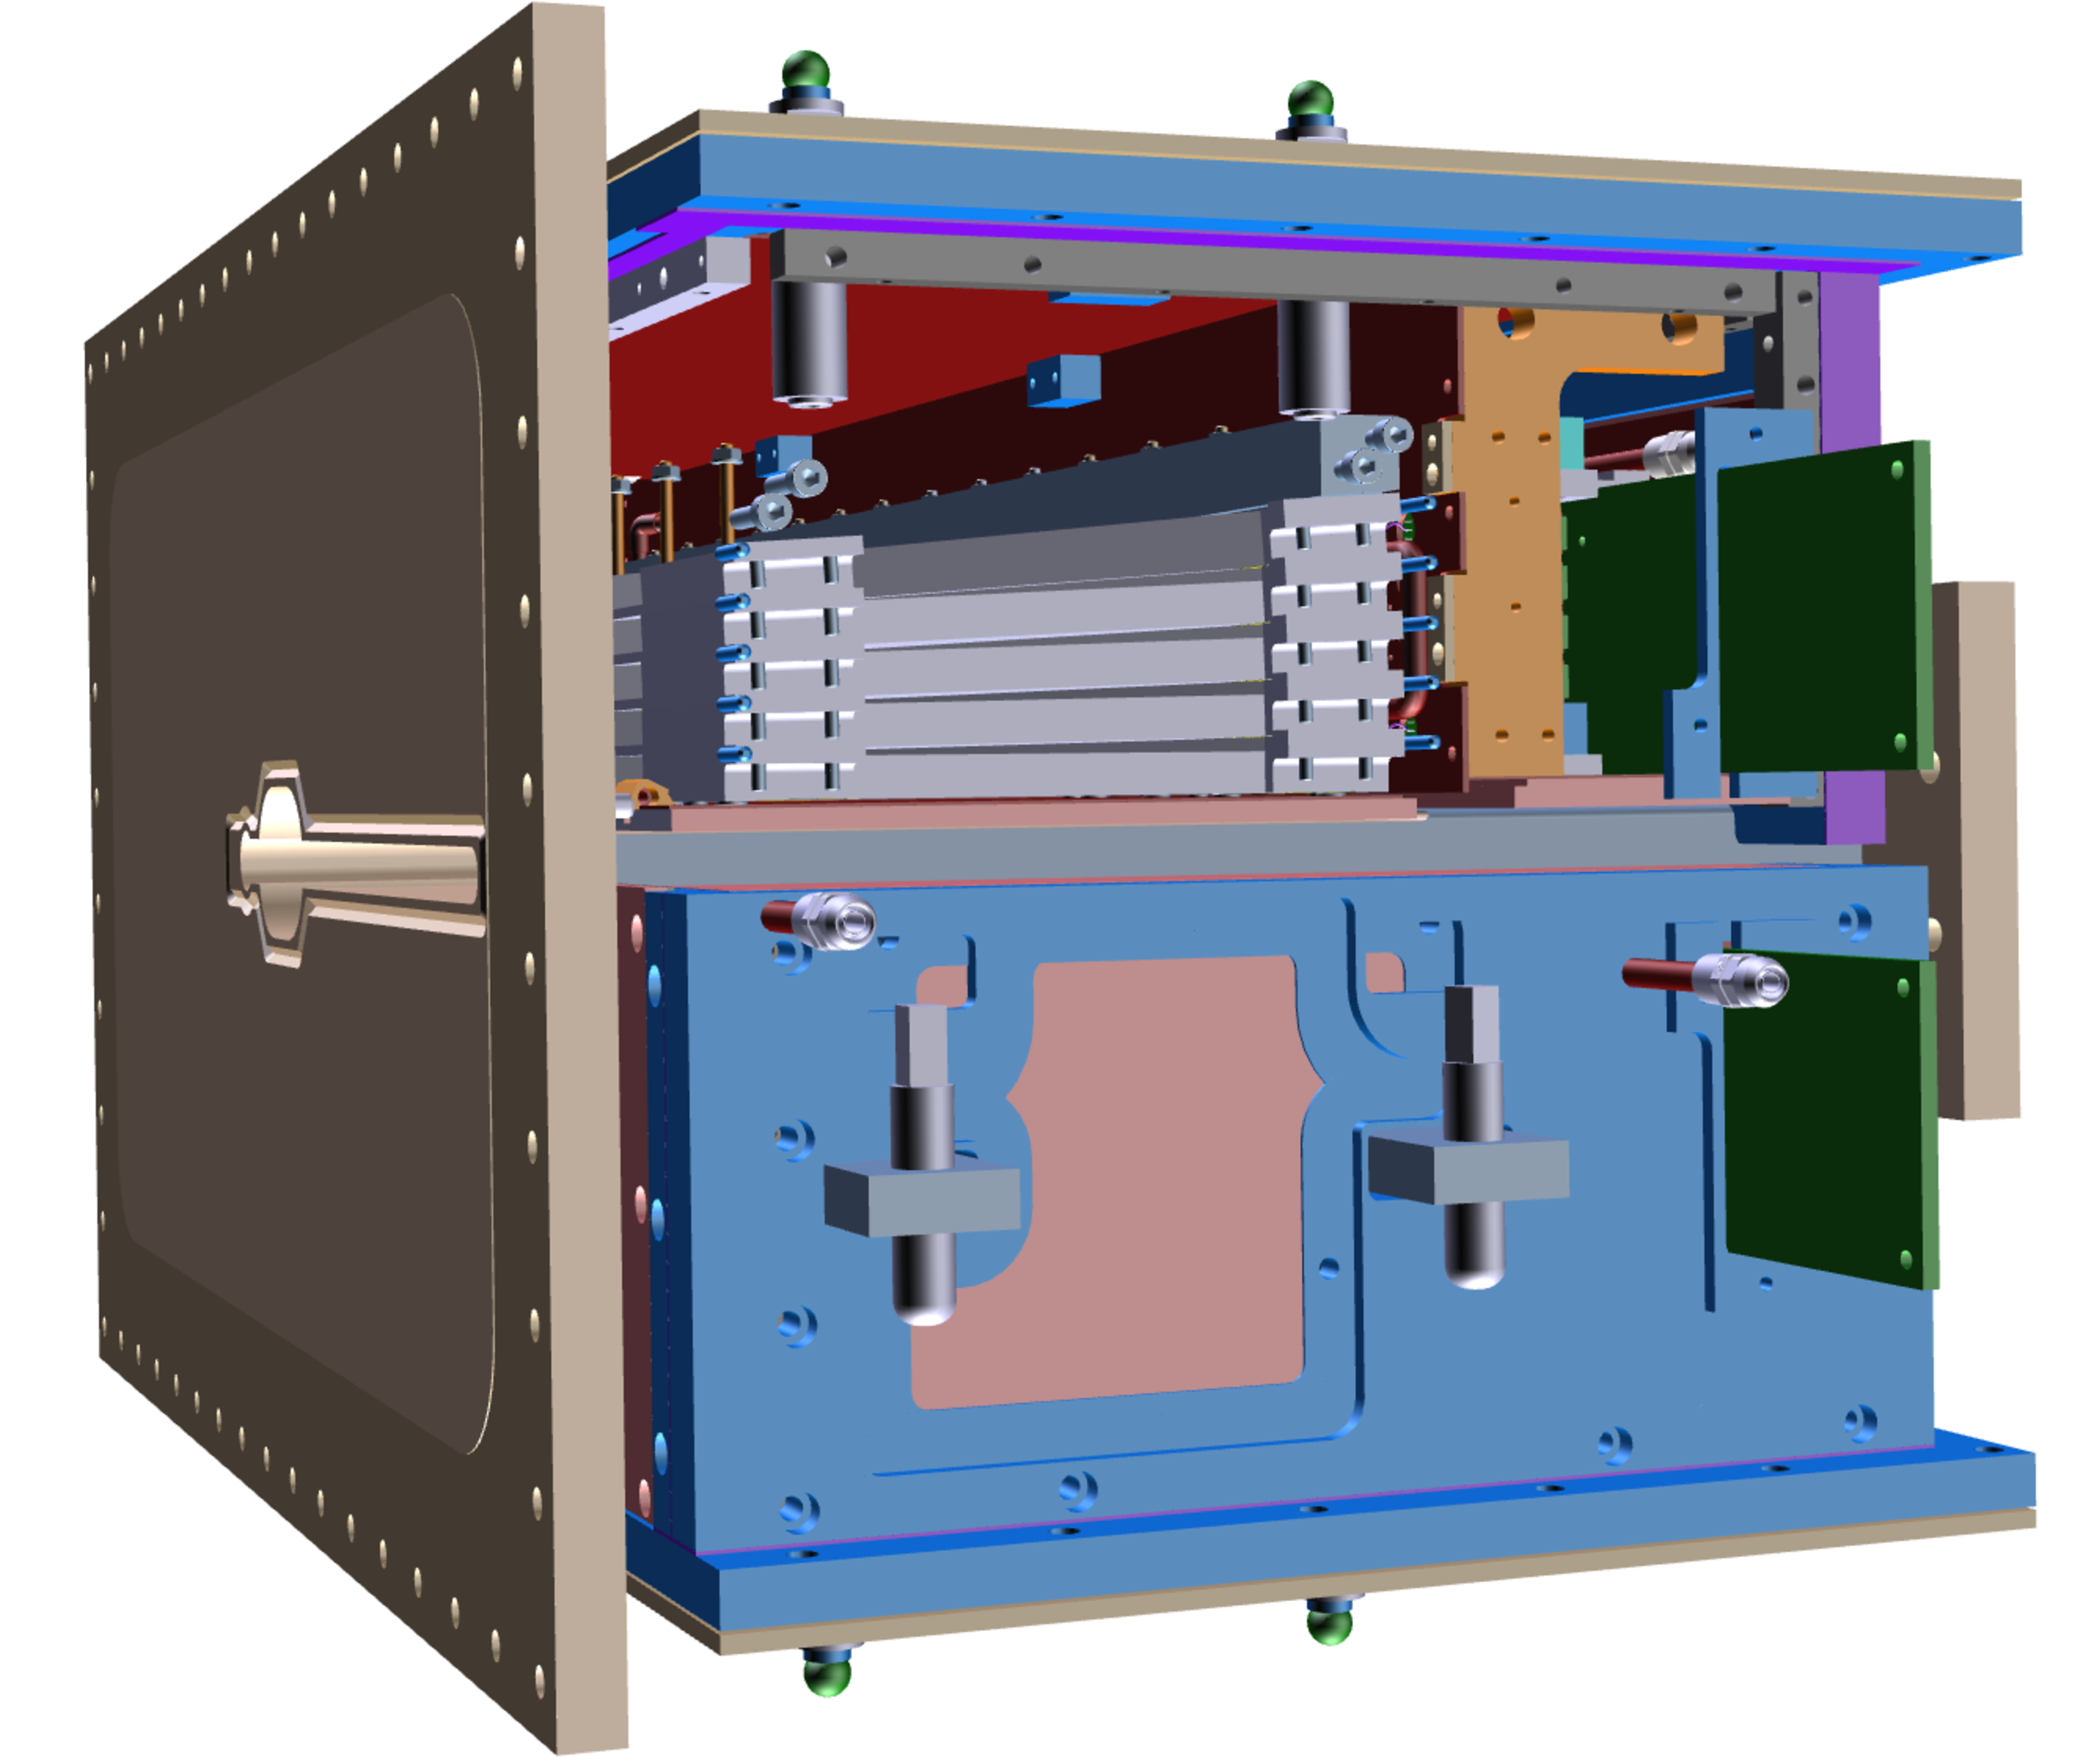
\includegraphics[width=7cm]{figures/ecal_vacuumchamber.pdf}
%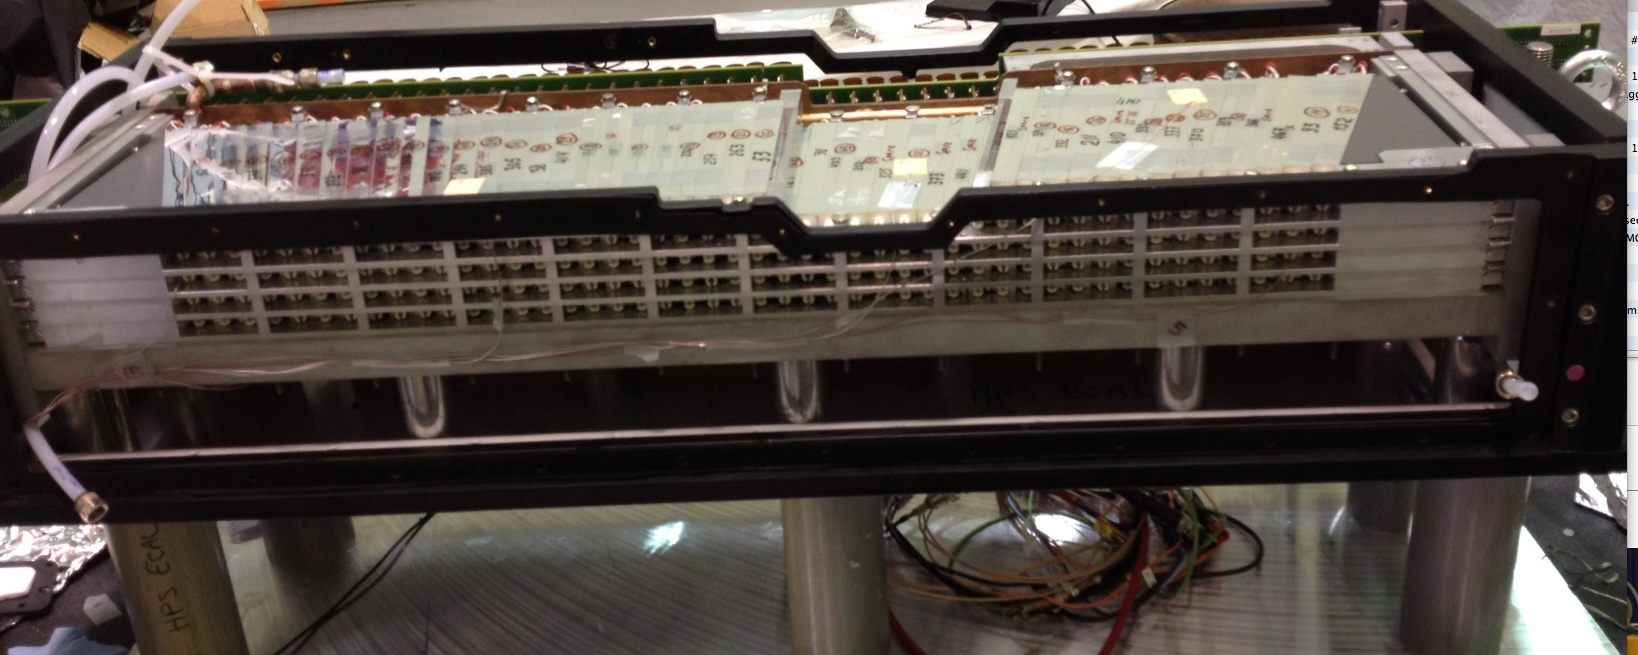
\includegraphics[width=7cm]{figures/ecal_assembly}
\caption{Layout of PbWO$_{4}$ modules in two halves of the ECal (left) and the ECal assembly on the beam line (right). }
\label{fig:ecal}
\end{figure*}
}
\end{center}
%Step \subsubsection{Support Structure}
%Step In order to stabilize the calorimeter's performance, the crystals, APDs, and amplifiers are enclosed within a temperature controlled environment, held constant at the level of .
%Step\subsubsection{Avalanche Photodiode Readout and Preamplifiers}
%Step\label{sec:apd}
%StepAvalanche Photodiodes (APD) S8664-55 produced by Hamamatsu Corp. are used as photodetectors. They have a $5\times5$~mm$^2$ active area and quantum efficiency of about 75\%. Single APDs were centered on the back ends of the crystals using MeltMount 1.7 thermal plastic adhesive. The low? amplitude signals of APDs are amplified using custom?made preamplifier boards. 
%The gain uniformity of the APDs is on the order of XXXX\%; with APD high voltage bias varying by as much as 100V. Since only a limited number of high voltage channels were available during the test, 10 channels were grouped together with an attempt to group modules with similar gains. 

\subsection{Signal readout}
\label{sec:fadc}

ECal signal readout was organized as follows: the amplified APD signal from the motherboard is sent to a $2:1$ signal splitter. After the split, 2/3 of the signal is sent a discriminator then to a Time-to-Digital 
Converter (TDC). The 1/3 of the signal is fed to a single channel of 16-channel JLAB Flash Amplitude-to-Digital Converter (FADC250), see Fig.\ref{fig:fadc} \cite{fadc}.  
\begin{figure}[t]
\begin{center}
{\small
\includegraphics[width=5cm]{figures/FADC250_Photo_001.jpg}
\caption{A Jefferson Lab FADC250 VXS module.}
\label{fig:fadc}
}
\end{center}
\end{figure}
Two 20-slot VXS crates with 14 (for top ECal) and 13 (for bottom ECal) FADC bards were employed for the test run. 

The FADCs store 12-bit digitized samples at 250~MHz in 8~$\mu$s deep pipelines. 
When a trigger is received, the appropriate part of the pipeline is accessed for the readout. HPS used 
FADCs in the integration mode. A predefined number of samples of the signal that exceeds a predefined 
threshold have been summed and stored in 17-bit register for readout. The number of samples for 
integration was defined by two parameters that could be set separately, the number of samples 
integrated before the signal crossed threshold ($NSB$) and  the number of samples integrated after the 
signal crossed threshold ($NSA$), see Fig.\ref{fig:hps_trigger_data}. 
\begin{figure}[]
\begin{center}
{\small
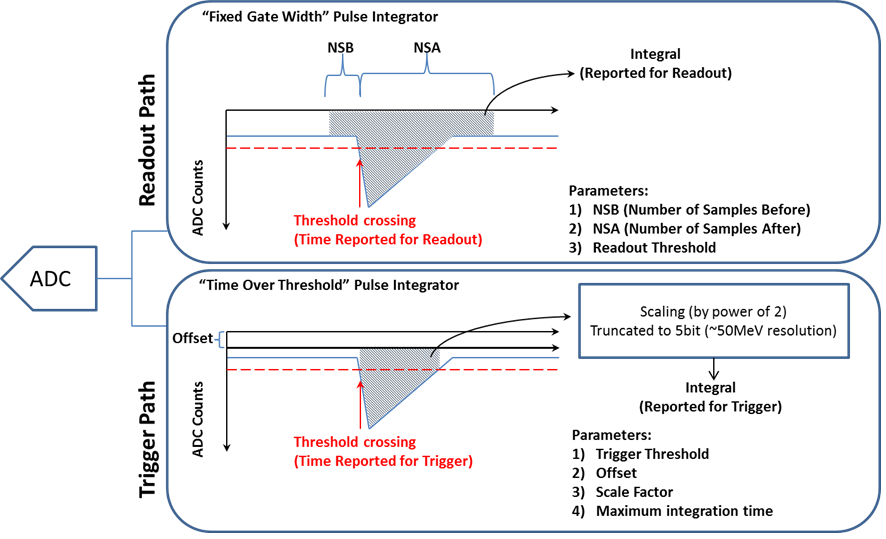
\includegraphics[width=7cm]{figures/fadc_datapath_diagram.png}
\caption{\small{FADC data paths.}}
\label{fig:hps_trigger_data}
}
\end{center}
\end{figure}
This scheme significantly compresses the data input to the FADC. During data analysis, a pedestal 
value is subtracted to obtain the actual summed energy.

For various reasons only 385 out of 442 modules (87\%) were operational during the test run. The 
readout threshold was set to $70$ MeV, the number of samples before and after the threshold crossing 
were 5 and 30, respectively. 


%%%%%%%%%%%%%%%%%%%%%%%%%%%%%%%%%%%%%%%%%%%%%%%%%%


\section{Trigger and Data Acquisition}

The HPS Test apparatus DAQ handles the acquisition of data from two sub-detectors: the 
SVT and the ECal, with two DAQ architectures. The SVT is readout with Advanced 
Telecom Communications Architecture (ATCA) hardware while the ECal uses VXS based 
hardware. The trigger system receives input from the ECal and distributes a trigger signal 
to all detector sub-systems to read out a selected event. 

\subsection{Trigger system}
\label{sec:trigger}

The HPS test run trigger system is designed to select \ee{} events efficiently by 
using information from the ECal. The trigger looks for time coincidences of clusters in the top and bottom 
half of the ECal. The trigger system can be broken down into three sections as shown in 
Fig.~\ref{fig:hps_trigger_cal}:
 \begin{figure}[b]
\begin{center}
{\small
 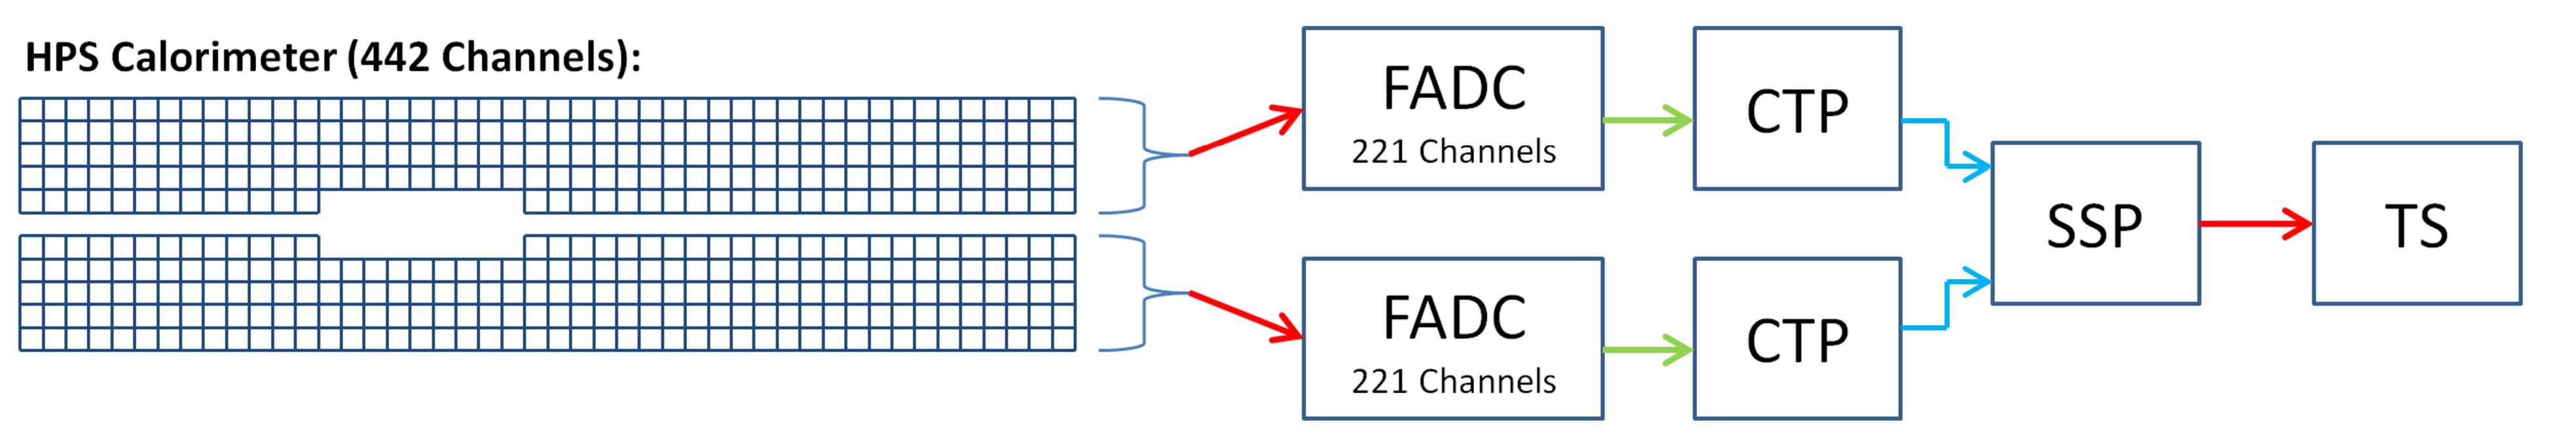
\includegraphics[width=8cm]{figures/hps_trigger_cal}
\caption{Block diagram of the ECAL trigger system consisting of the FADC that samples and digitizes 
signals for each detector channel and sends them for cluster finding in the CTP. The CTP clusters are 
sent to the SSP where the final trigger decision is taken based on pairs of clusters in both halves of the 
ECal. The decision is sent to the Trigger Supervisor (TS) that generates the necessary signals to readout 
the sub-detectors.}
 \label{fig:hps_trigger_cal}
}
\end{center}
 \end{figure}
 \begin{itemize}
 \item FADC (pulse finding): samples and digitizes the signal pulses from each detector channel. 
Sends the measured pulse energy and arrival time to the Crate Trigger Processor (CTP),
\item CTP (cluster finding): groups FADC pulses from each half of the ECal into clusters. 
The cluster energy and arrival time are sent to the Sub-System Processor (SSP),
 \item SSP (cluster pair finding): searches for time coincidences of pairs of clusters from 
the top and bottom half of the ECal and applies topological selections.
 \end{itemize}

The time coincidence window of pairs of clusters in the top and bottom half of the ECal are 
programmable with 4~ns resolution.  As described above, the first stage of the trigger logic is 
incorporated into the FPGA's on the FADC boards. The trigger  
integrates using a "time-over-threshold" window as explained in Fig. \ref{fig:hps_trigger_data}.
For triggering purposes, every channel has: 
\begin{itemize}
% \item number of samples integrated before the threshold crossing (NSB),
 %\item number of samples integrated after the  threshold crossing (NSA),
 \item a trigger threshold, measured in ADC counts, 
 \item an offset, 
 \item a conversion factor to convert ADC counts into energy in MeV, from $50$ to $\sim1500$~MeV, with 5-bit accuracy 
 \item an energy threshold discriminator to provide aminimum energy cutoff
 \end{itemize}
Note that the threshold for the trigger path can be set independently from the readout threshold.
The offset is subtracted from ADC samples before they are integrated.  
The values reported to the CTP are the 5-bit pulse energy and the 3-bit time at which the 
pulse crossed the threshold. Data from every channel is sent to the CTP every 32~ns. With the available 
3-bit time information, the CTP looks for time coincidences of crystal signals within an 8~ns window (the 
limit is 4~ns).
The cluster finding algorithm is fast and makes use of the parallel processing capability of the FPGA's by 
simultaneously searching for 125 clusters, up to 3x3 in size, across the calorimeter crystal array, and it 
performs the following tasks:
\begin{itemize}
\item Adds together the energy for every 3x3 square of channels in the ECal
\item Hits are added together if their leading edges occurred within a programmable number of 4~ns 
clock cycles  (HPS test run used 8~ns coincidence time interval).
\item If the 3x3 energy sum is larger than the programmable cluster energy threshold and the sum is 
greater than any neighboring 3x3 windows, the CTP reports the cluster parameters to the SSP. 
\end{itemize}
The CTP evaluates all the hits in its half of the calorimeter every 4~ns. A programmable time window is 
used to allow hits that are slightly out of time with each other to be considered as part of a cluster sum. 
This is done by reporting hits when they occur and then reporting them again for the next $N$ number of 
4~ns clock cycles, where $N \in [0,7]$. This is useful to deal with skew and jitter that develop from the 
detector, cabling, and electronics. As described above, the CTP only selects the 3x3 window with the 
highest energy sum of its neighbors. This filtering is applied to deal with overlapping clusters and cases 
where the cluster is larger than a 3x3 window.

The final trigger decision is made by CTPs and the SSP is passed to the Trigger Supervisor (TS). The TS 
generates all necessary signals and controls the entire DAQ system readout through the Trigger 
Interface (TI) units. The TI units are installed in every crate that participate in the readout process. 

The trigger system is free-running and driven by the 250~MHz global clock and has essentially zero 
dead time at the occupancies expected for HPS. The Trigger Supervisor can apply dead time if 
necessary, for example on a `busy' or `full' condition from the front-end electronics. The system is 
designed to handle trigger rates above 50~kHz and has a latency set to $\approx 3~\mu$s to match that 
required by the SVT APV25 chip. 

During the test run, for the most part the trigger system required only a single cluster in either the top or 
bottom Ecal module. It was tested to work up to 20 kHz trigger rates. 

\subsection{Data Acquisition and Online Computing}
\label{sec:daq}
For the ECal, every VXS crate contains a Readout Controller (ROC)
that collects digitized information, processes it, and sends it on to the Event Builder (EB). The ROC is a 
single blade Intel-based CPU module running DAQ software under CentOS Linux OS. For the SVT 
ATCA system, the ROC application runs on an embedded processor situated on the ATCA main board. 
The EB assembles information from the SVT and ECal ROCs into a single event which is passed to the 
Event Recorder (ER) that writes it to a RAID5-based data storage system capable of handling up to 
100~MB/s. The EB and other critical components run on multicore Intel-based multi-CPU servers. The 
DAQ network system is a network router providing high-speed connections between the DAQ 
components and the JLab computing facility. The SVT ROC, which must handle large data volumes, has 
a 10~Gbit/s link to the network router, while a 1~Gbit/s link is adequate for the ECal. A 10~Gbit/s uplink 
to the JLab computing facility is used for long-term storage.

The SVT DAQ is described in more detail in Sec.~\ref{sec:svt_daq}.





%%%%%%%%%%%%%%%%%%%%%%%%%%%%%%%%%%%%%%%%%%%%%%%%%%


\section{Performance}

\subsection{SVT Performance}

During the duration of the test run all SVT modules and APV25 chips were configured to their 
nominal operating points~\cite{Jones:1069892} with all sensors reverse-biased at 180~V.  The 
sensors were operated within a temperature range of  $20-24^\circ$C 
throughout the test run. 
Throughout the duration of the test run, approximately 97\% of the 12,780 SVT channels were found to
be operating normally. The fraction of dead or noisy channels varied from 2.4\% to 4.7\%.  
Most of these were due to misconfigured readout chips (2--4 misconfigured chips out of 100 ), 
a known noisy half-module and a couple of known noisy readout chips. 


\subsubsection{Cluster and Hit Reconstruction}

After a trigger is received, six samples of the corresponding output of the APV25 shaper circuit are digitized. The samples from every channel on a sensor surviving the 
data reduction algorithm (see Sec.~\ref{sec:svt_daq}) are the basis for offline hit reconstruction. 
The six samples of the APV25 shaper output 
are fitted to an ideal $CR-RC$ function to extract the amplitude and the $t_0$ of the hit. 
The typical pulse shape obtained is shown in Fig.~\ref{fig:pulse_shape} also demonstrates that the SVT 
was well timed in to the trigger with the rise of the pulse at the 3rd sampling point.
\begin{figure}[]
\begin{center}
{\small
	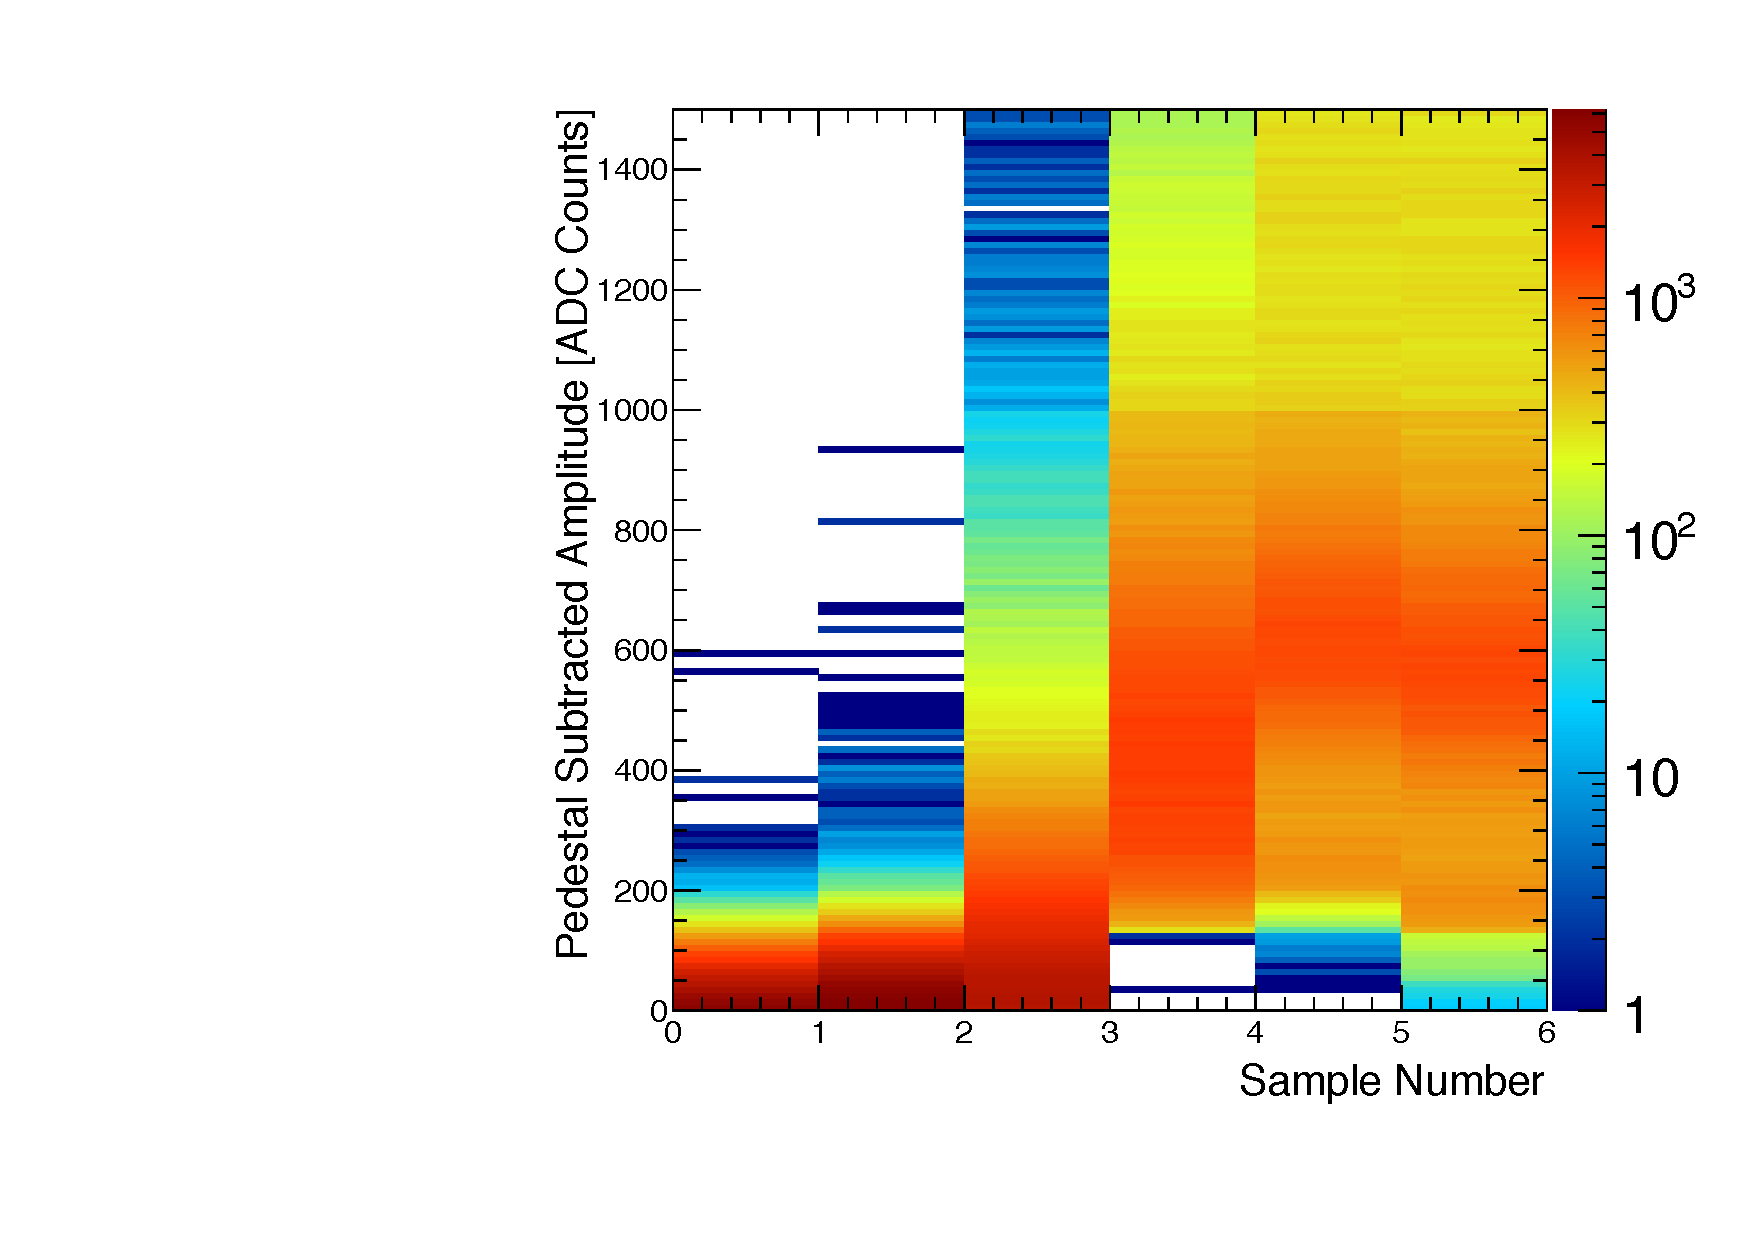
\includegraphics[width=6cm]{figures/run1351_110513_samples_L1_top.pdf}
	\caption{The six pedestal subtracted samples from individual channels associated with a hit on a 
	track.}
	\label{fig:pulse_shape}
}
\end{center}
\end{figure}

These hits are passed through a simple clustering algorithm which forms clusters by grouping adjacent 
strips. The position of a cluster on the sensor is determined by the amplitude-weighted mean.
With a linear gain up to $\approx 3$~MIPs, the cluster charge for hits associated with a track follow 
the characteristic Landau shape as expected, see Fig.~\ref{fig:cluster_pulse}.  
A noise level between $1.1-1.5\times 10^{3}$ electrons was established through multiple calibration 
runs giving a signal to noise ratio of $21-25$. Lab-based radioactive source tests was used to 
provide the absolute charge normalization.
\begin{figure}[]
\begin{center}
{\small
	%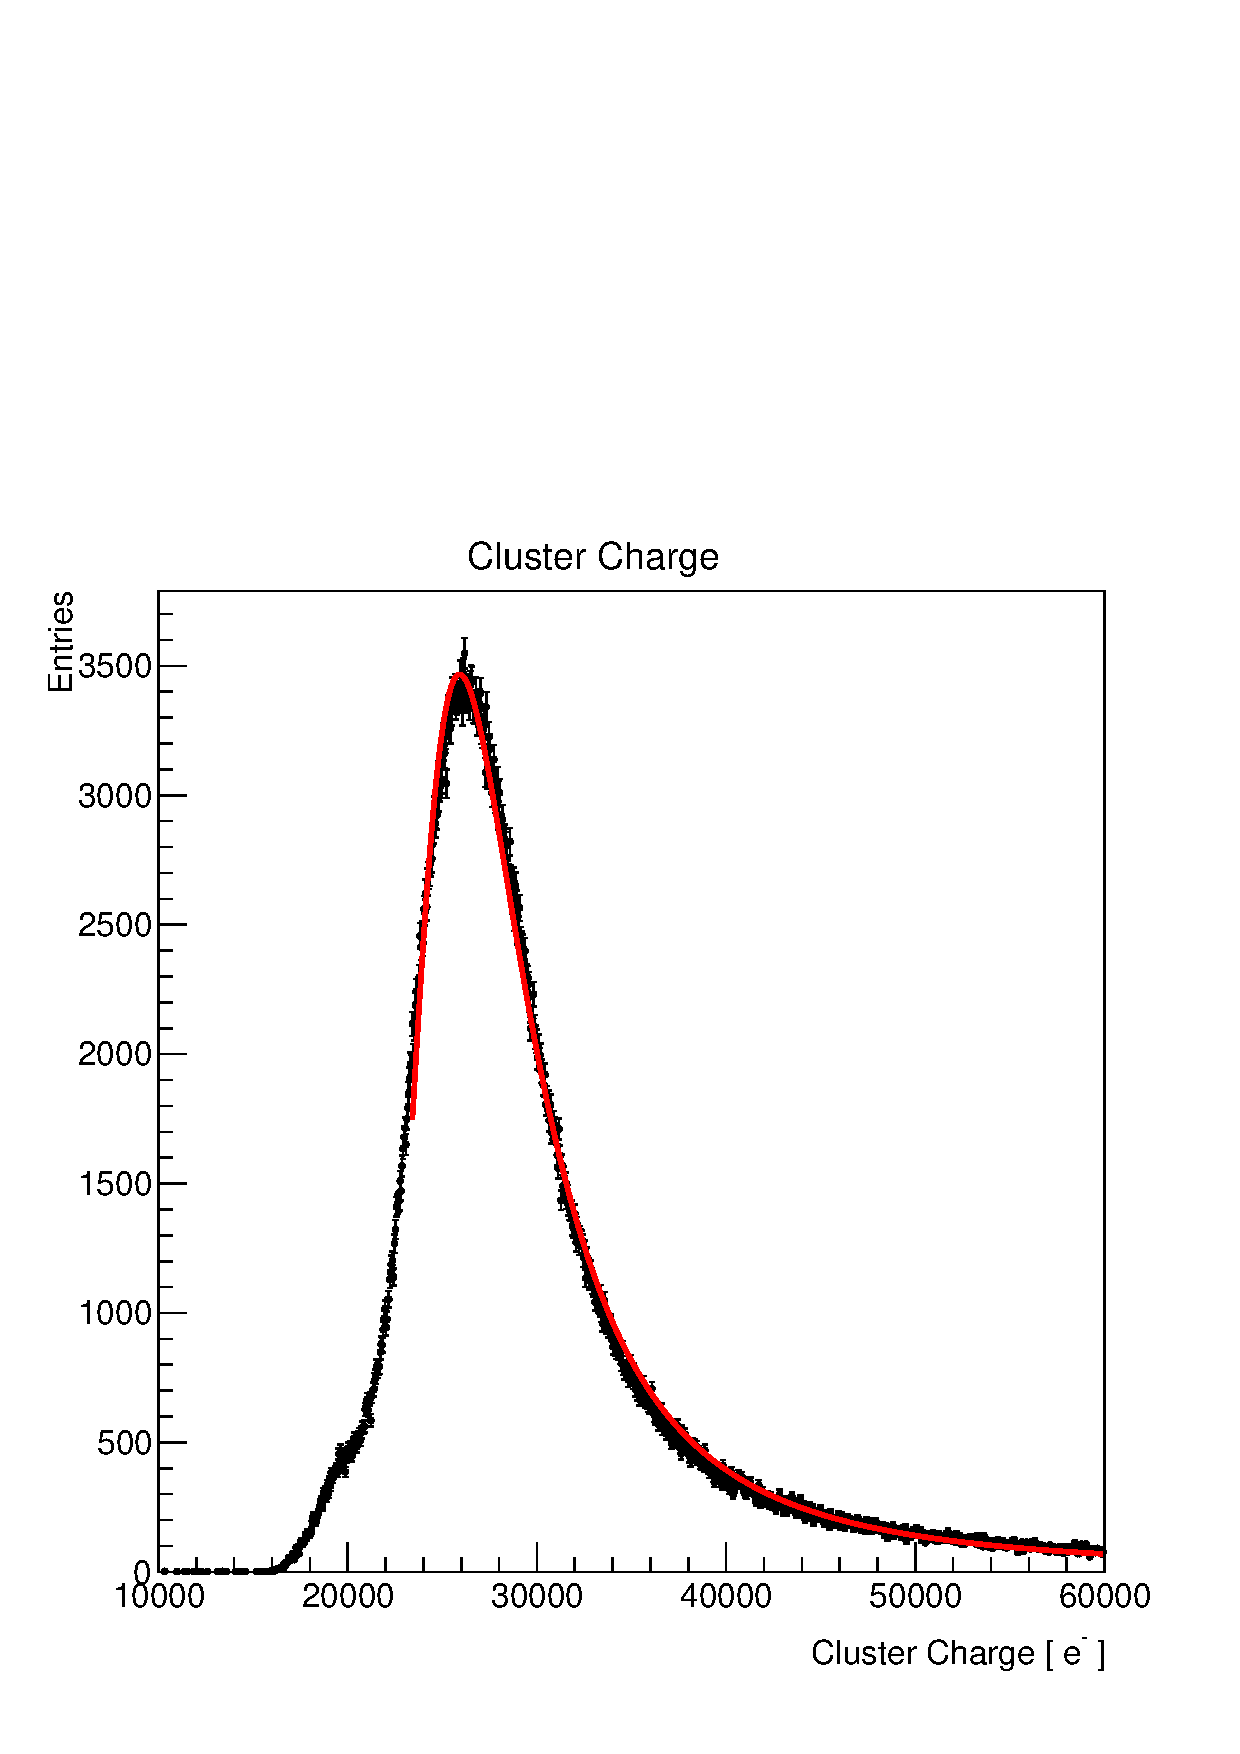
\includegraphics[width=7cm]{figures/run1351_mip_small.pdf}
	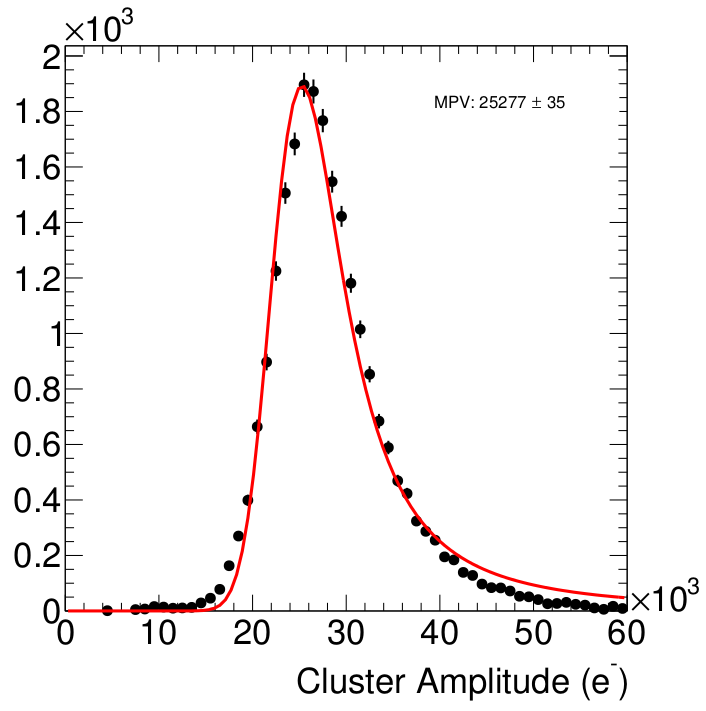
\includegraphics[width=7cm]{figures/mip_top_layer_2.png}
    	\caption{ The cluster charge distribution for hits associated with a track. }
	\label{fig:cluster_pulse}
}
\end{center}
\end{figure}

After clustering hits on a sensor, the hit time for each cluster is computed as the amplitude-weighted 
average of the fitted $t_0$ channel times. The $t_0$-resolution is studied by comparing the cluster hit 
time with the average of all cluster hit times on the track, the ``track time'', which has the expected jitter 
due to clock phase and trigger, approximately 25~ns. Figure~\ref{fig:tracktime} shows the residual to the individual cluster 
times. 
\begin{figure}[]
\begin{center}
{\small
	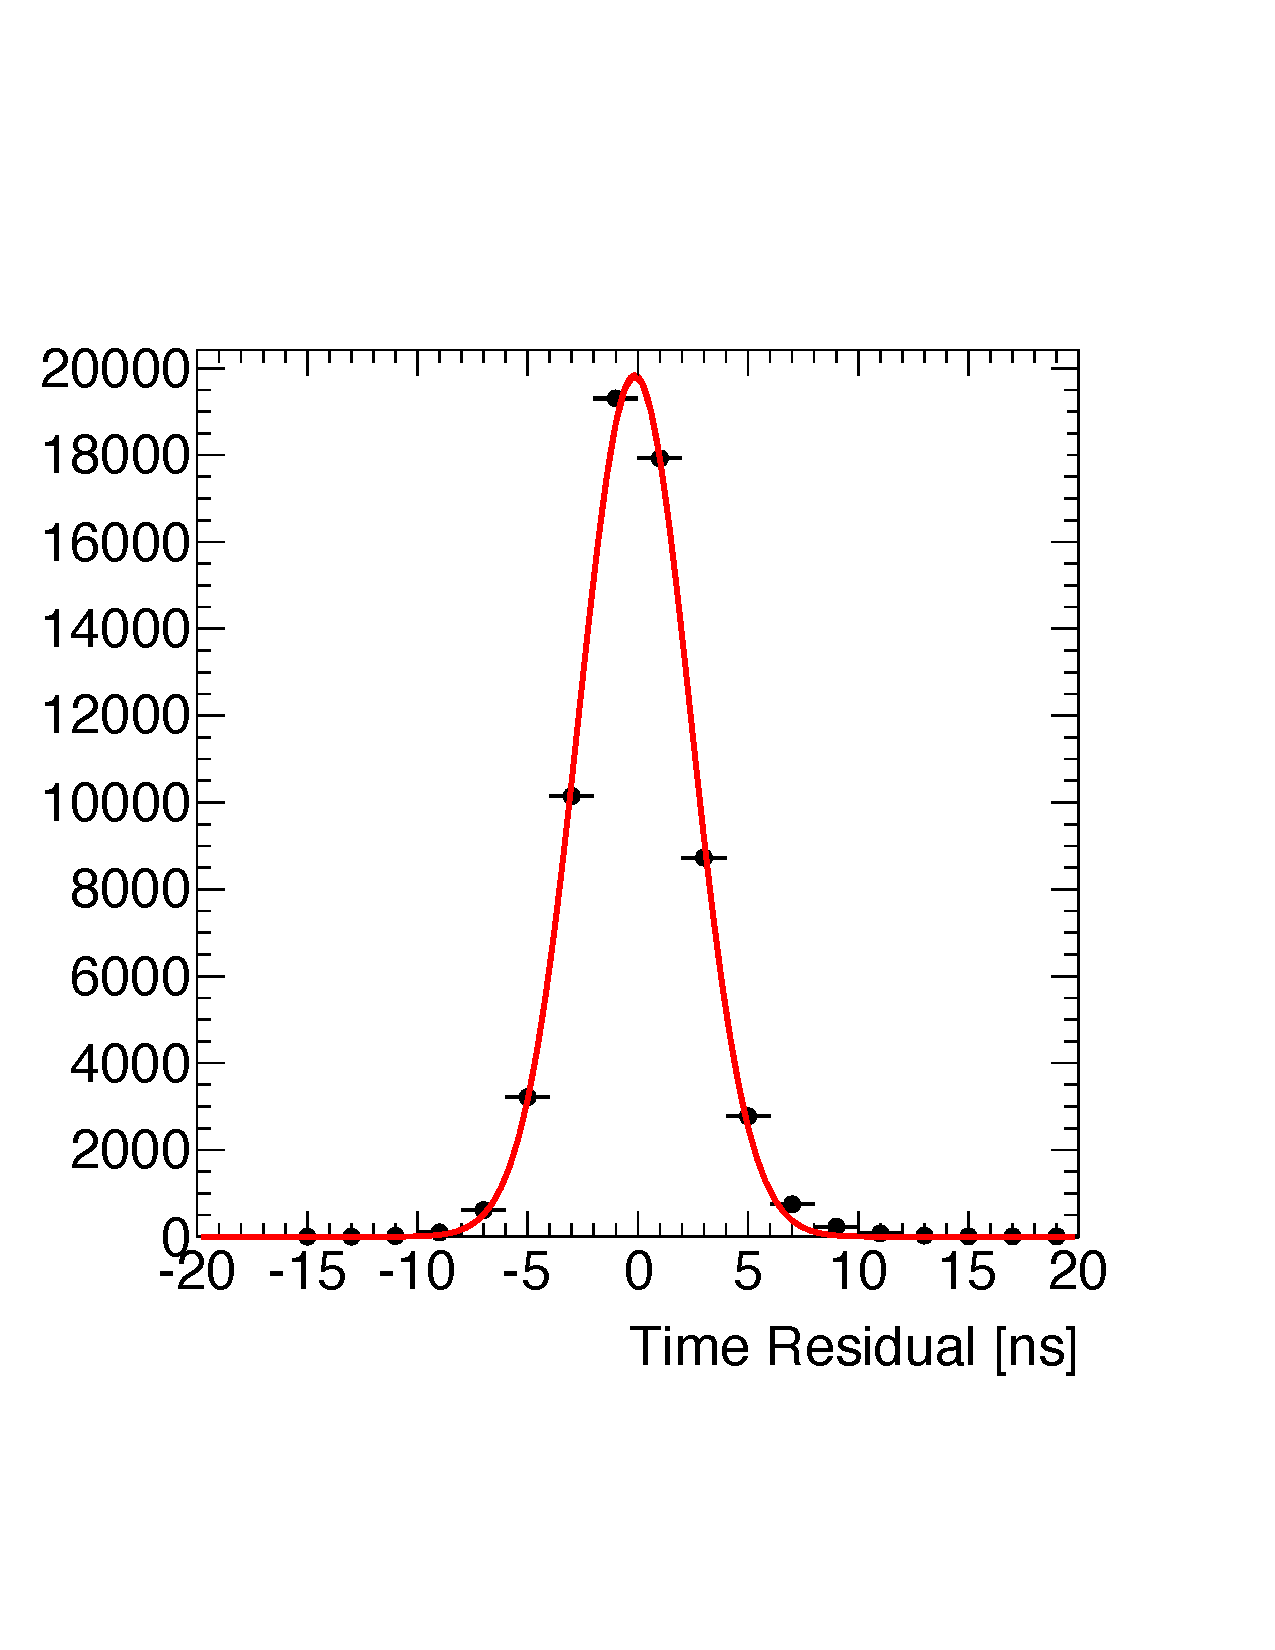
\includegraphics[width=7cm]{figures/test_run_1351_hit_time_corrected_top_layer2_mod.pdf}
	\caption{
	The cluster time residual for a representative sensor relative to the track time (see text for more 
	details). }
	\label{fig:tracktime}
}
\end{center}
\end{figure}
After correcting for offsets from each sensor (time-of-flight, clock phase) and accounting for the 
correlation between the $t_0$ and track time,  the extracted $t_0$ resolution is 2.6~ns. This is somewhat 
worse than the approximately 2~ns resolution expected which we attribute to the true 
pulse shape differing from our idealized fit function which will be improved in the future. Reducing the 
APV25 pulse shaping time will also improve time resolution. These results show that we can operate 
with the six sample readout mode of the APV25 chip and achieve time resolution adequate for pileup 
rejection during electron running in the HPS experiment. 

While occupancy was slightly larger than expected, good agreement between data and simulation was 
found after taking into account dead or noisy channels. The hit efficiency was estimated by measuring 
the number of good tracks with a hit close to the extrapolated intersection of a given sensor that was 
excluded from the track fit itself. Tracks which intersect regions with known bad channels or very close to 
in the edge region are excluded in the calculation of the single hit efficiency. The hit efficiency, see 
Fig.~\ref{fig:hit_efficiency}, was measured to be above 98\% and fairly uniform across the SVT.
\begin{figure}[]
\begin{center}
{\small
    	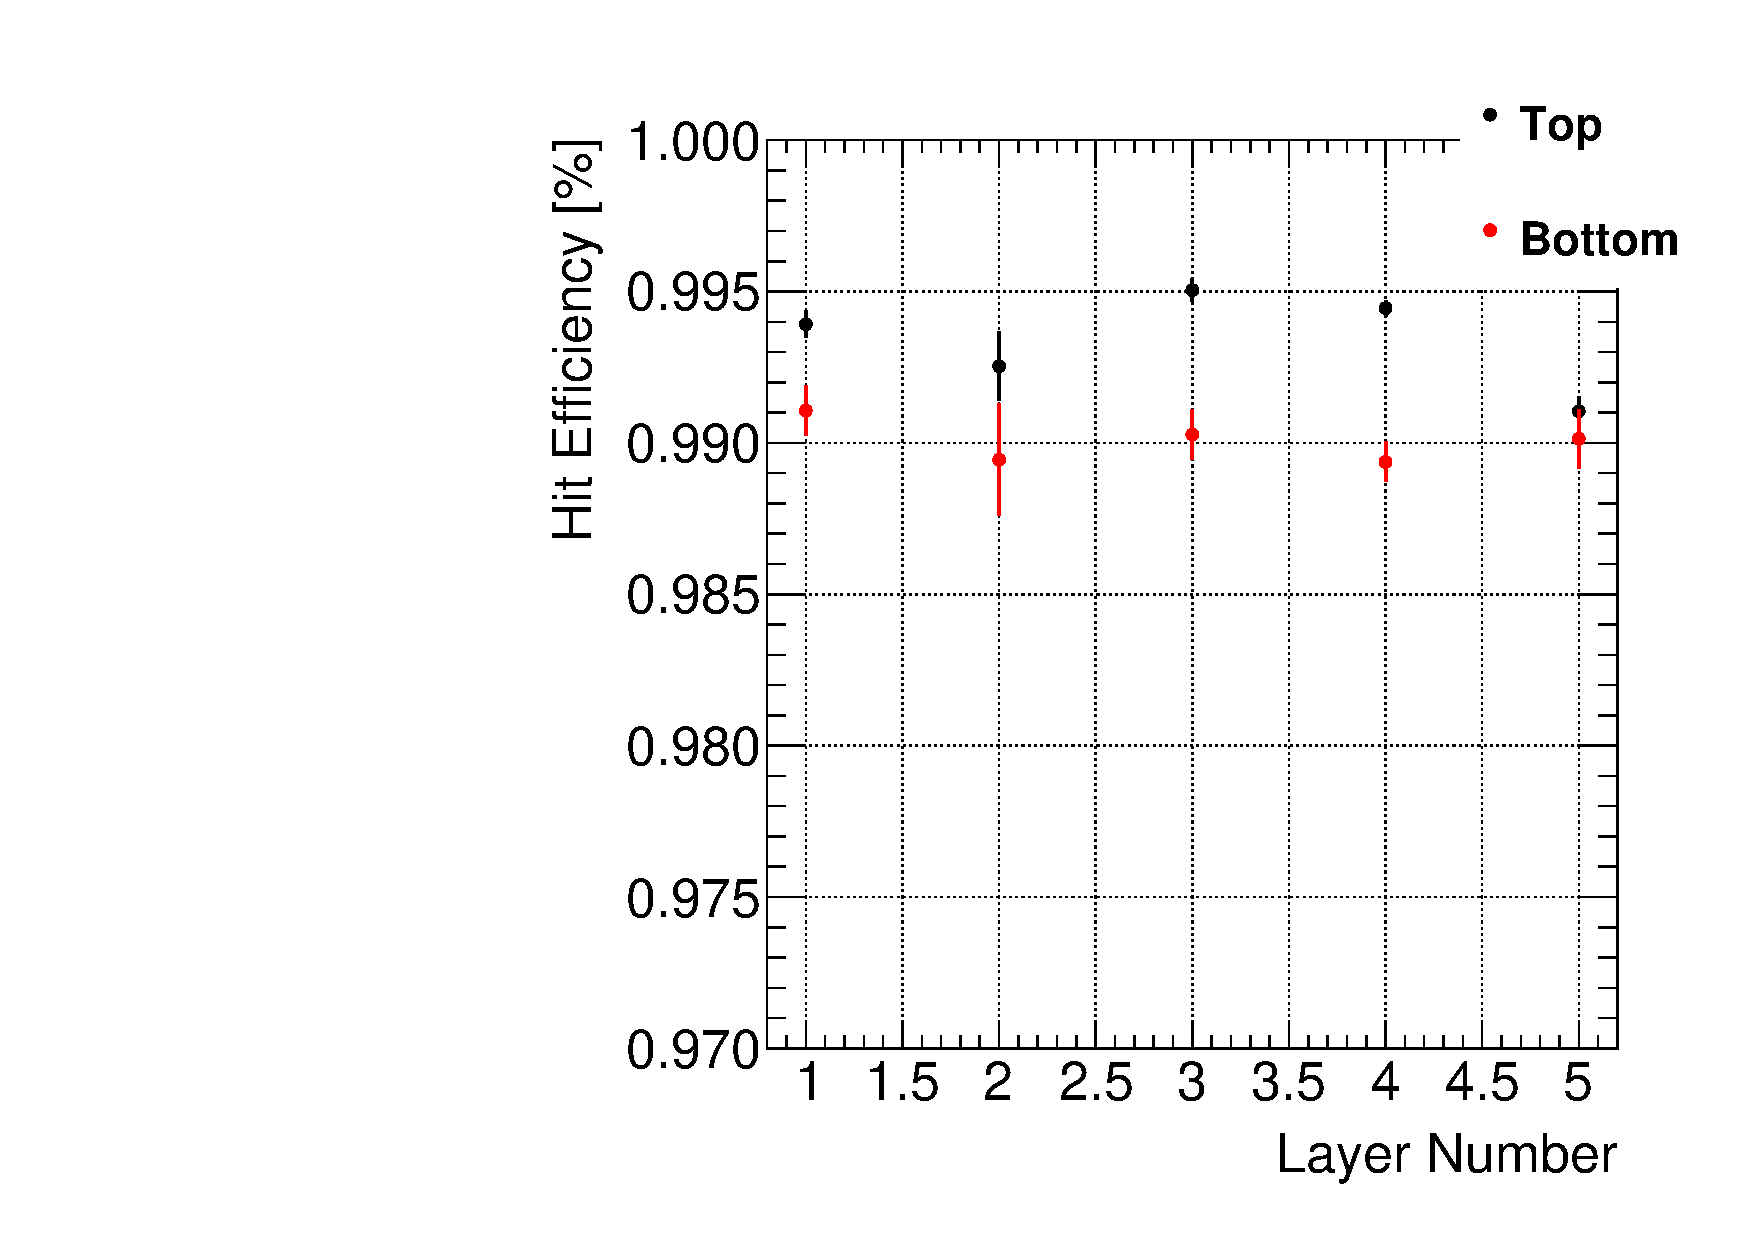
\includegraphics[width=7cm]{figures/single_hit_efficiency_Omar_11192013.pdf}
        \caption{ The hit reconstruction efficiency as a function of detector layer.}
	\label{fig:hit_efficiency}
}
\end{center}
\end{figure}
The spatial resolution of similar microstrip sensors is well established by test beam data, against which 
the charge deposition model in the simulation is validated.  This resolution can be parameterized as a 
function of the total signal to single-strip noise (S/N) and the crossing angle of tracks through the sensor.  
The single-hit resolution for charged particles with signal to noise ratio above 20, as demonstrated 
here, is relatively constant at approximately 6~$\mu$m for tracks that enters approximately normal to the 
sensors as in HPS.



\subsubsection{Momentum and Vertexing Resolution}

By selecting \ee{} pairs from the triggered events we are able to study basic distributions of pair 
production kinematics and in particular those related to our vertex performance. Pairs of opposite charge 
tracks, one in the top and one in the bottom half of the SVT, with momentum larger than 400~MeV were 
selected. The pair production kinematics are relatively well reproduced given the alignment of the 
tracker; Fig.~\ref{fig:pair_kin} shows the invariant mass and ratio of electron momentum over the sum of 
electron and positron. 
 \begin{center}
{\small
\begin{figure*}[t]
   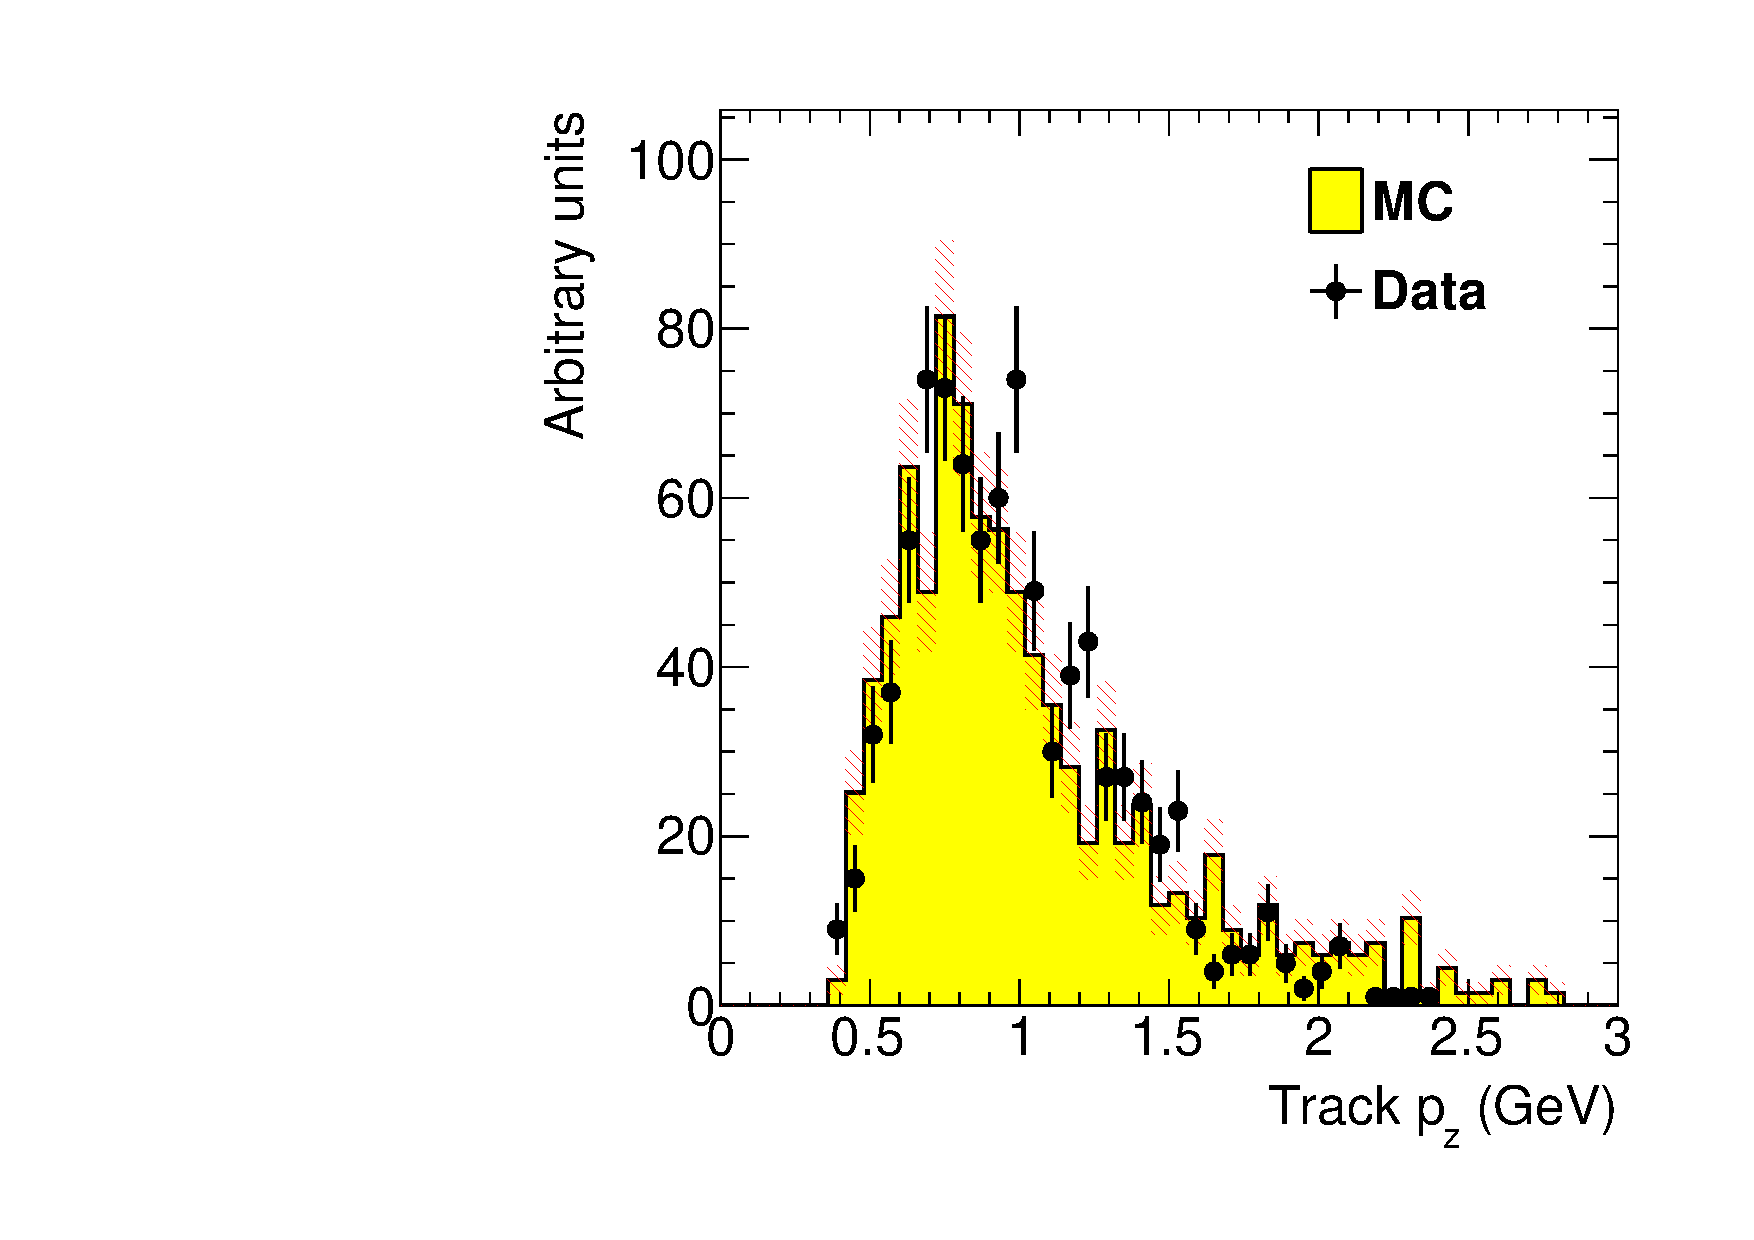
\includegraphics[width=5cm]{figures/h_trk_top_px_h_trk_top_px_trigsel4hit_pair1351_twotrkfilt-v6-paper}
   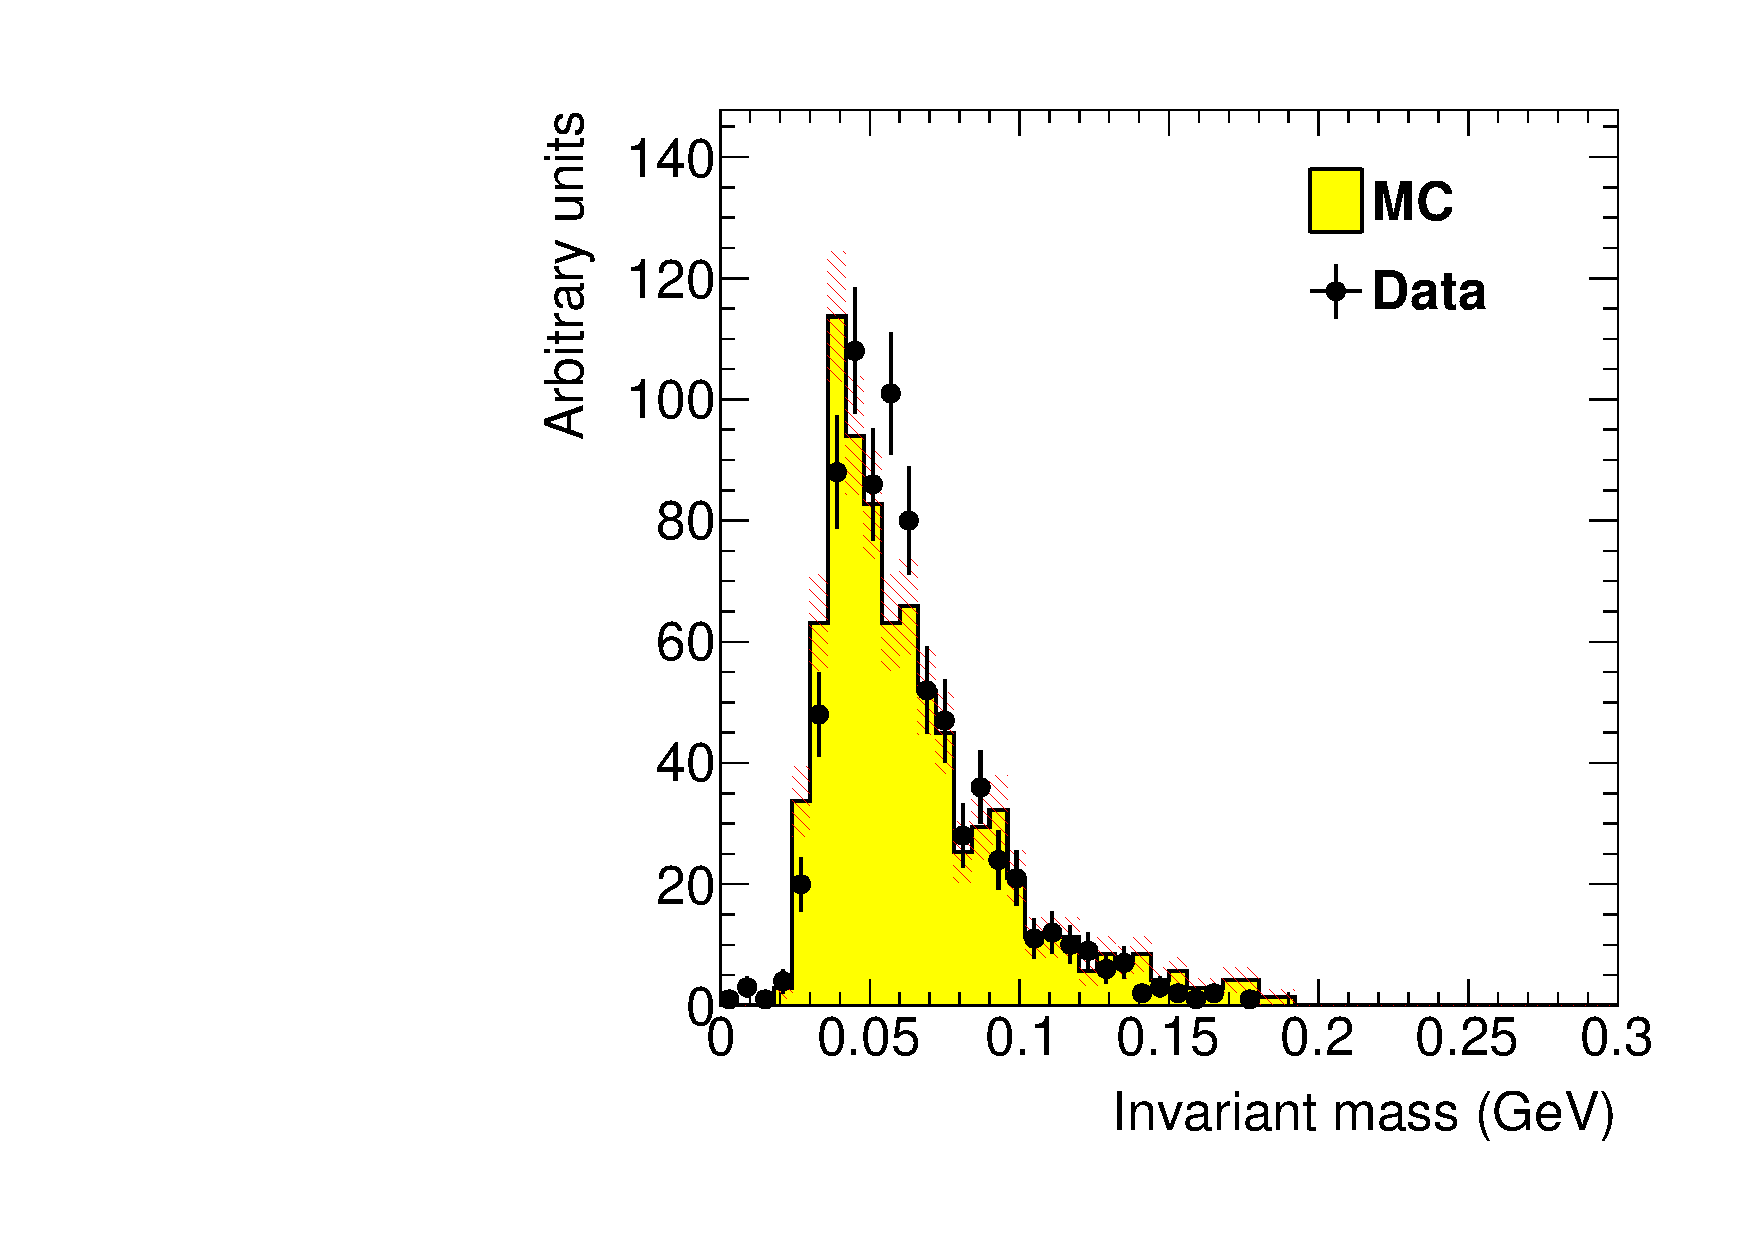
\includegraphics[width=5cm]{figures/h_invM_h_invM_trigsel4hit_pair1351_twotrkfilt-v6-paper}
   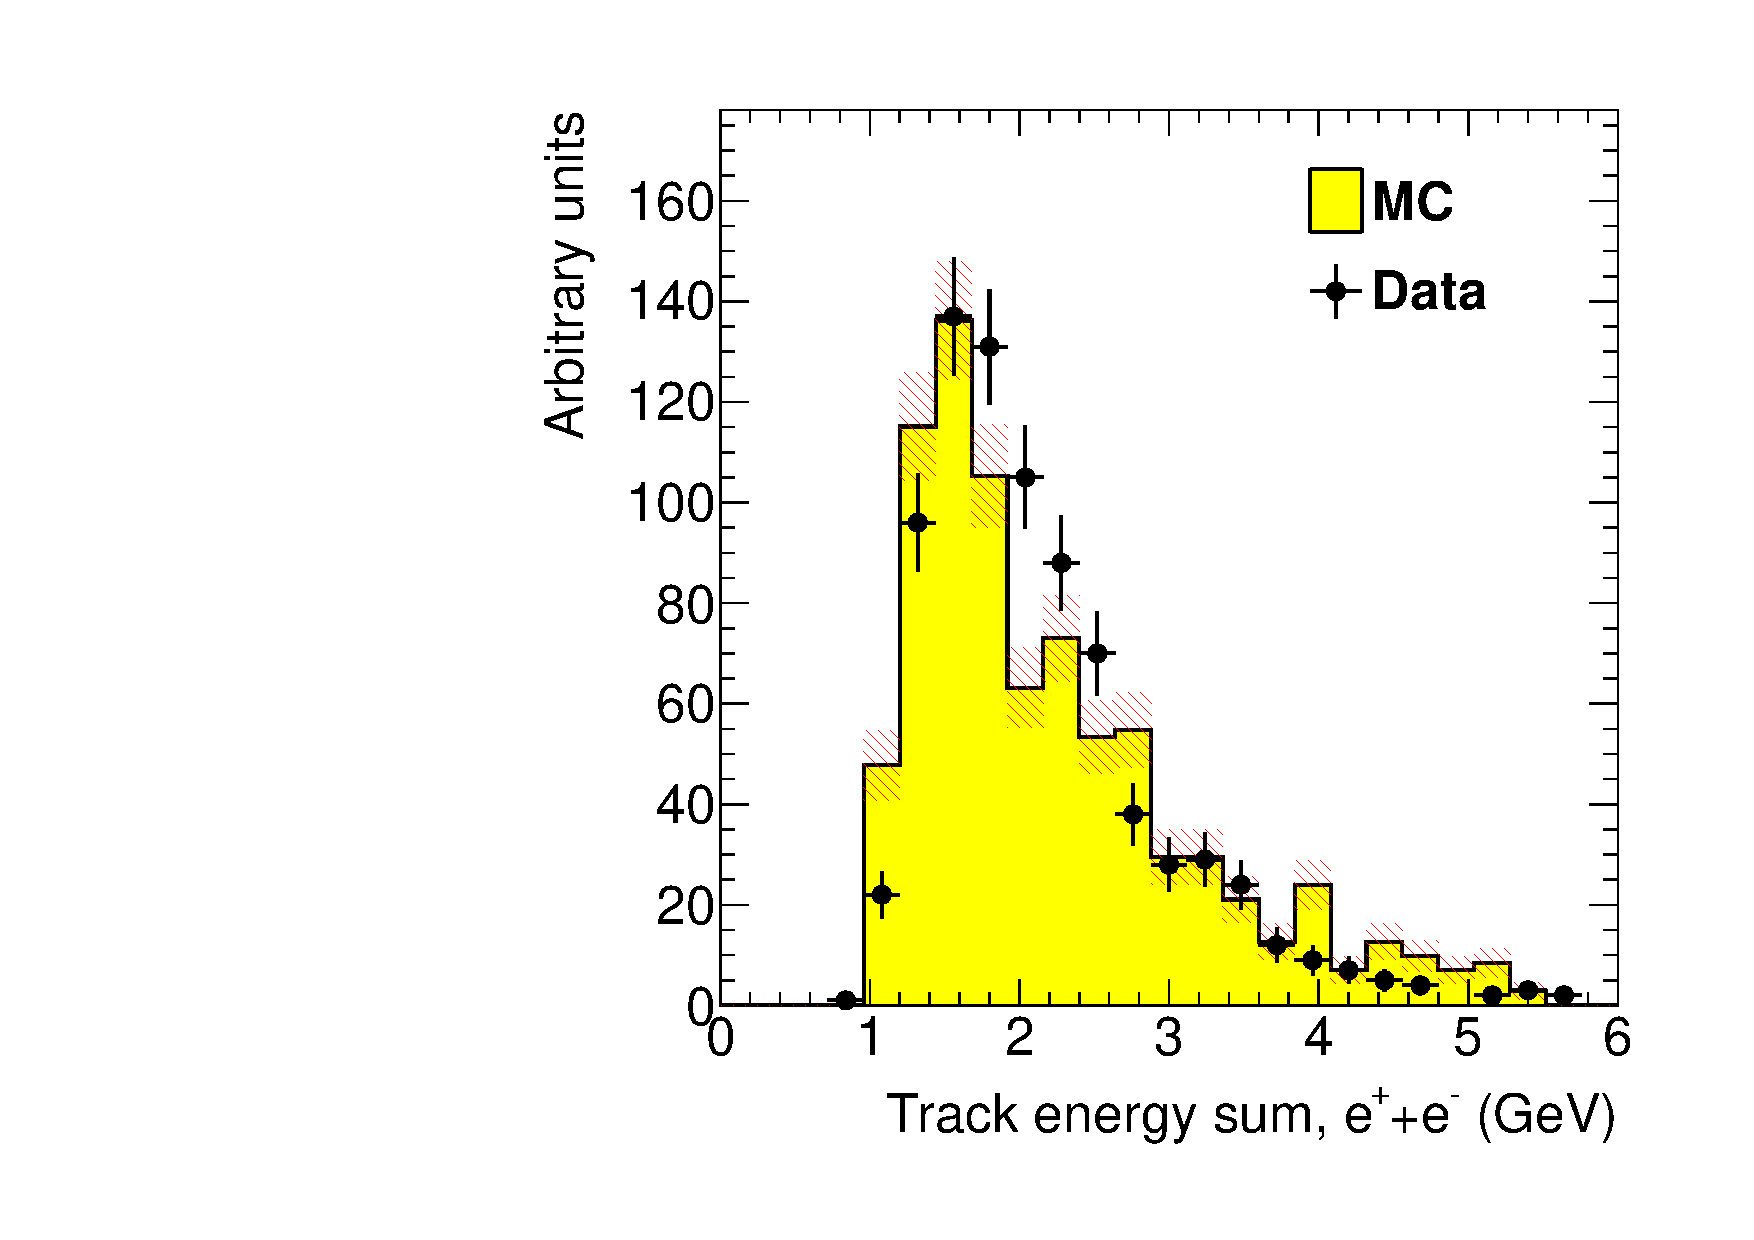
\includegraphics[width=5cm]{figures/h_sumE_h_sumE_trigsel4hit_pair1351_twotrkfilt-v6-paper}
\caption{Kinematic distributions for e$^+$e$^-$ pairs selected by opposite charged tracks in the top and bottom half of the tracker: track momentum in the top half of the SVT (left), invariant mass (middle) and the sum of the track momentum for the pair (right).}
\label{fig:pair_kin}
\end{figure*}
}
\end{center}
We estimate the accuracy of the SVT momentum scale and resolution by looking at the agreement 
between data and simulation in the shape of the kinematic distributions for single- and two track 
events.  By adjusting the overall momentum scale and smearing the simulated events with a 
Gaussian resolution we estimate an uncertainty of 10\% on both the momentum scale and 
resolution in the Test run. The expected momentum resolution from simulation is between 4-5\% 
for tracks in the momentum range of the Test run.

For the vertexing performance the foremost difference compared to electron beam running is that the 
target was located approximately 67~cm from our nominal target position; giving almost collinear tracks 
in the detector. This degrades the vertex resolution along the 
beam line compared to that expected in an electron beam with tracks from the nominal target position. 
Furthermore, tails of the vertex distributions are impossible to study with the finite data sample obtained 
in the Test run. Nevertheless, useful information can still be 
obtained by studying the vertex distributions. Figure~\ref{fig:vtx_pos} shows the distance of closest 
approach of the momentum vectors extrapolated in the upstream direction from our analyzing magnet, 
taking into account the measured fringe field of the PS magnet. 
 \begin{center}
{\small
	 \begin{figure*}[t]
	% Plot info:
	% TestRun-v6 geometry, twotrkfilter, trigsel, hps-java-1.8-SNAPSHOT, 4hits, chi2<10
	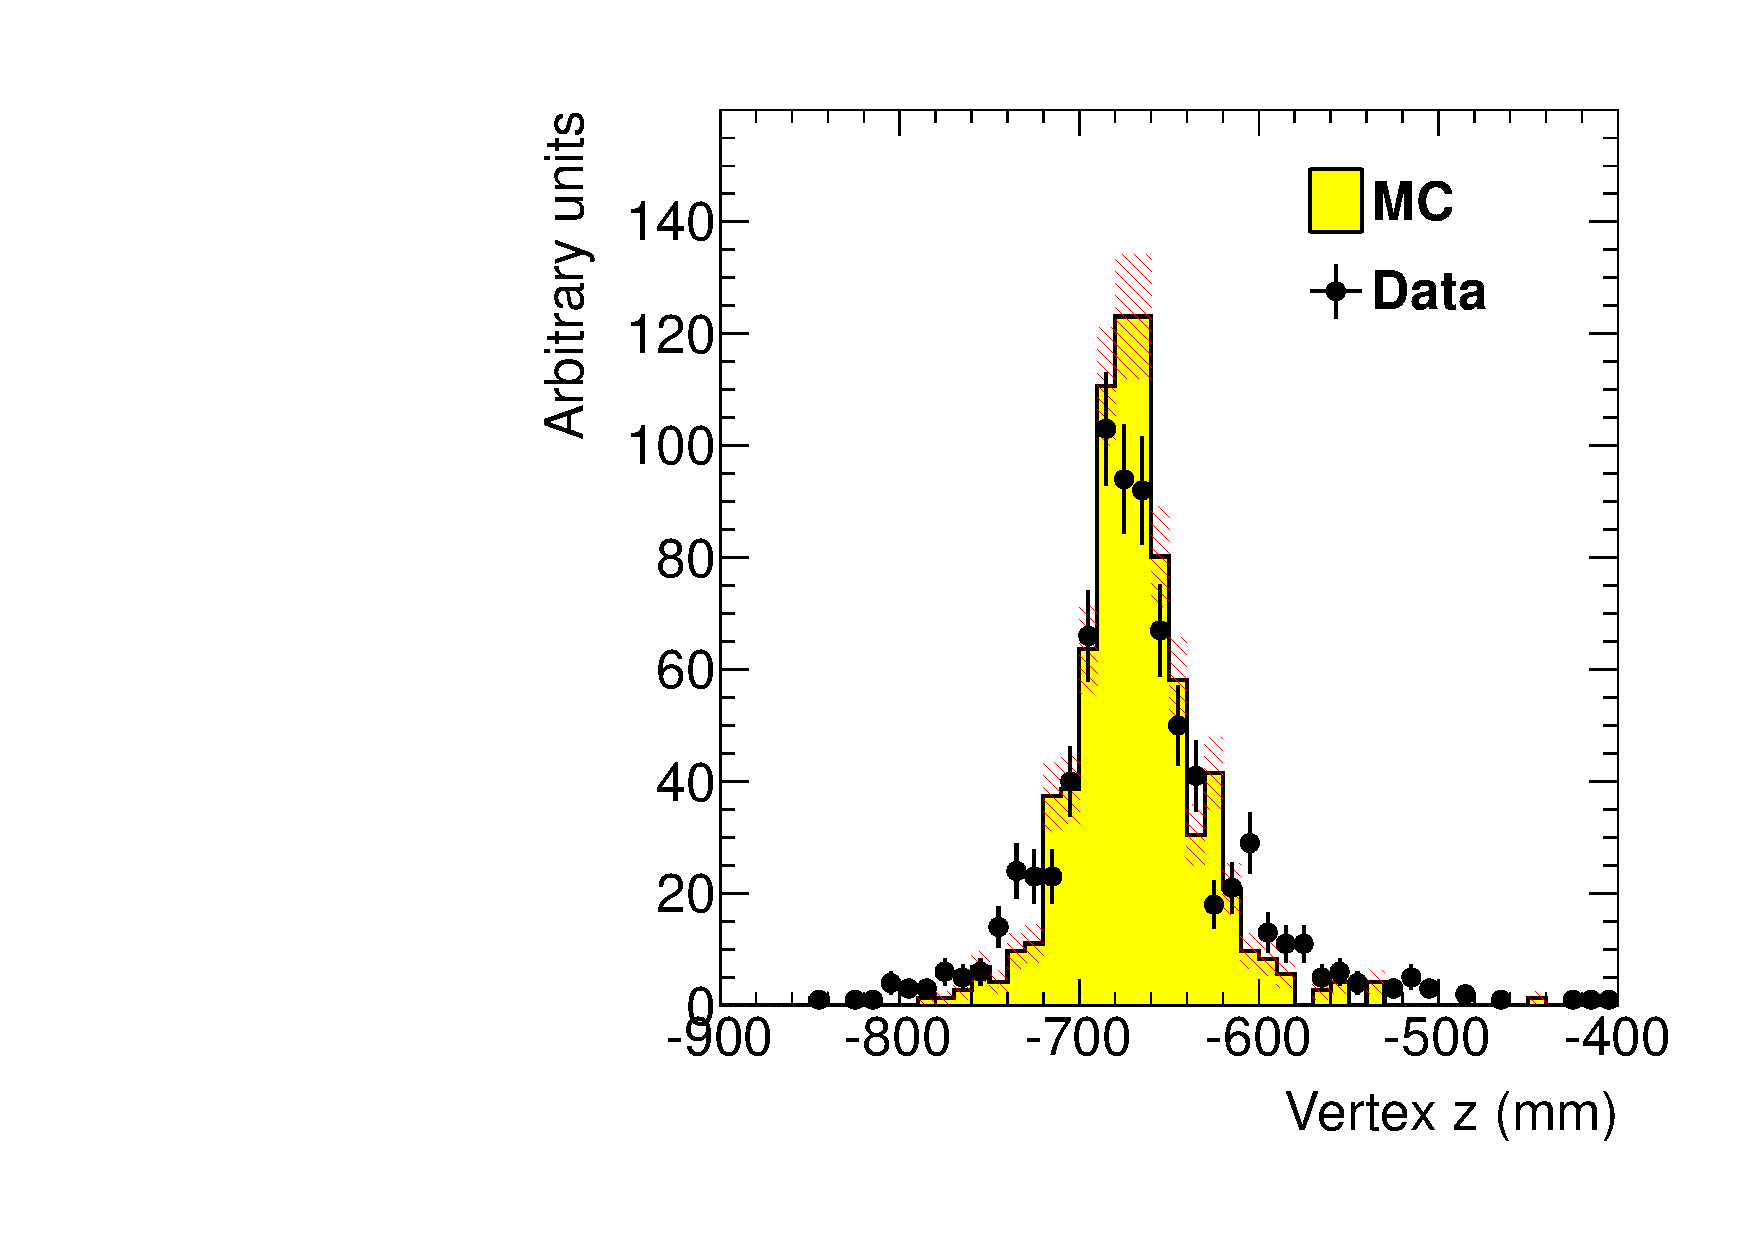
\includegraphics[width=5cm]{figures/h_vtx_fr_x_h_vtx_x_trigsel4hit_pair1351_twotrkfilt-v6-paper}
	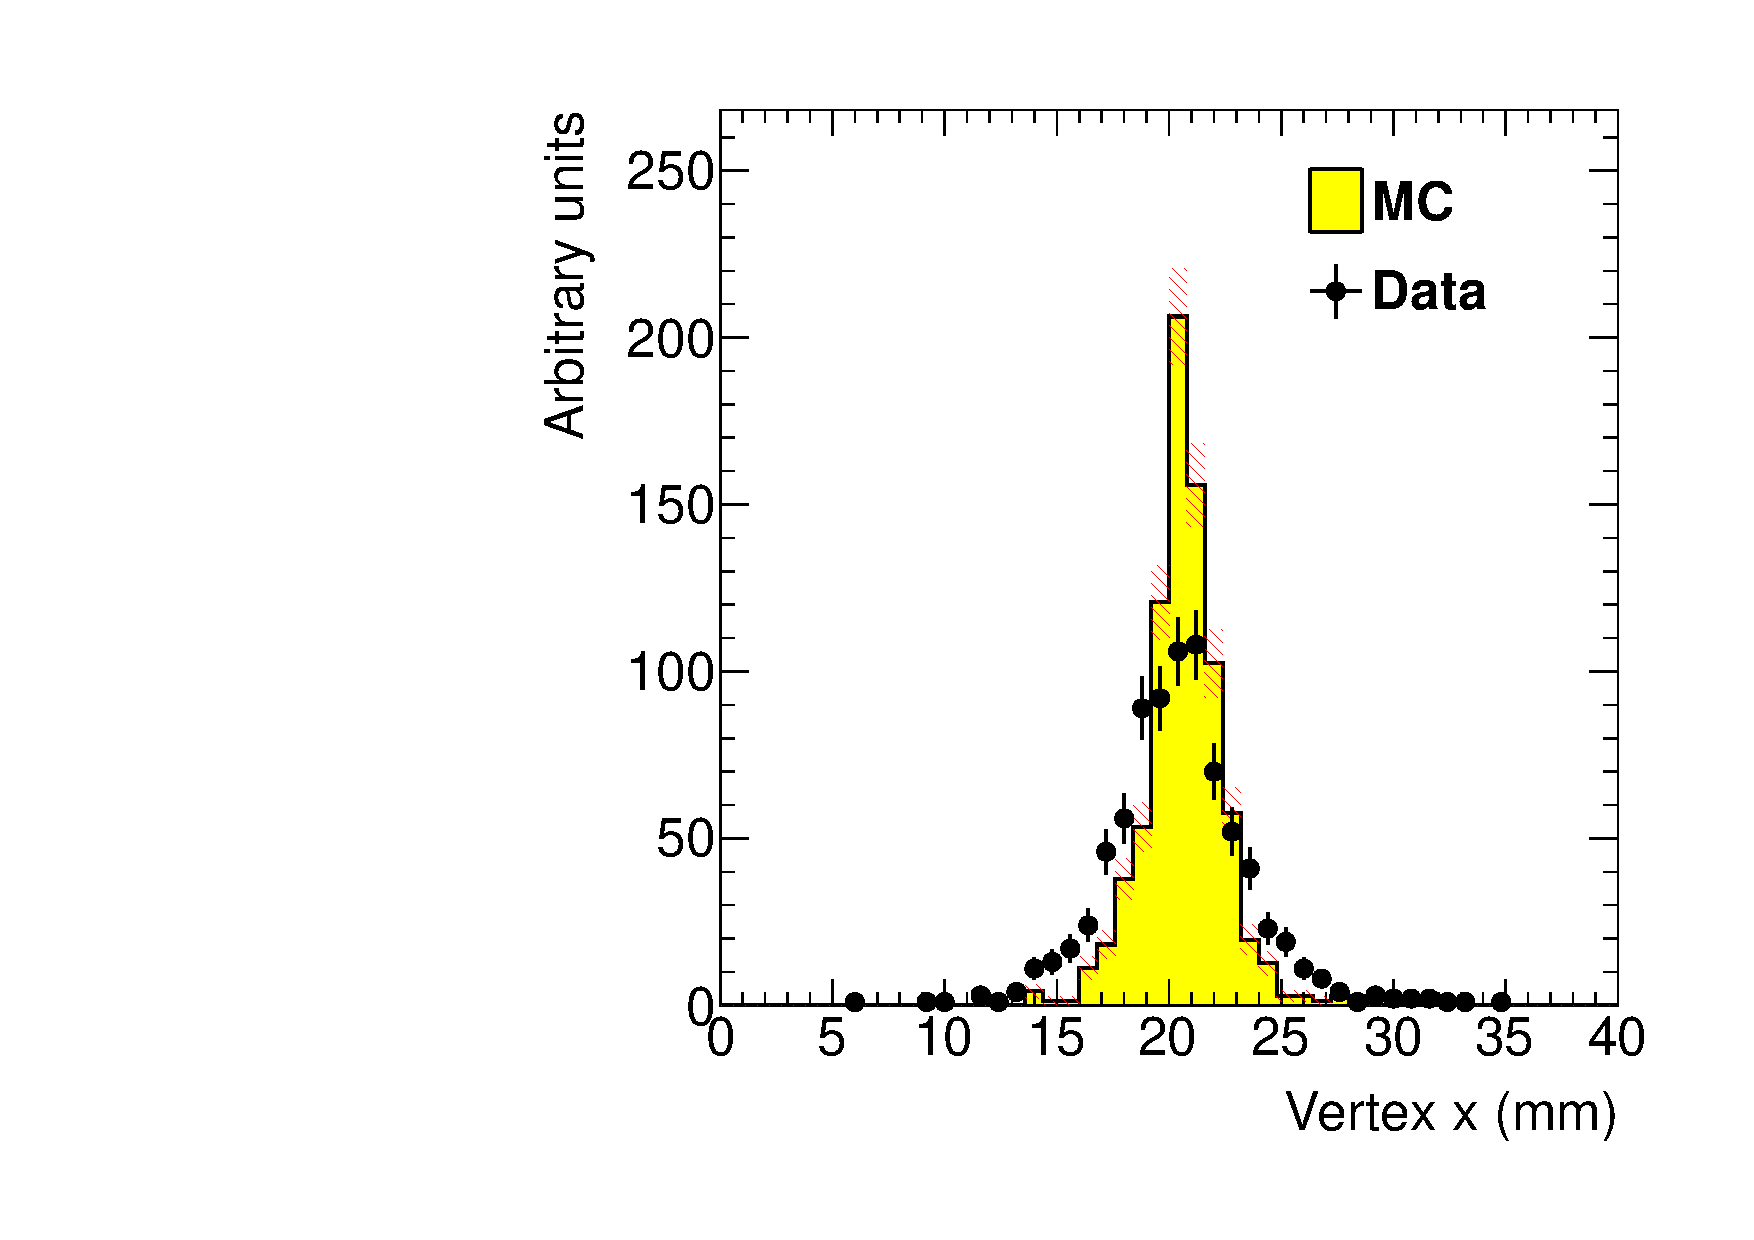
\includegraphics[width=5cm]{figures/h_vtx_fr_y_h_vtx_y_trigsel4hit_pair1351_twotrkfilt-v6-paper}
	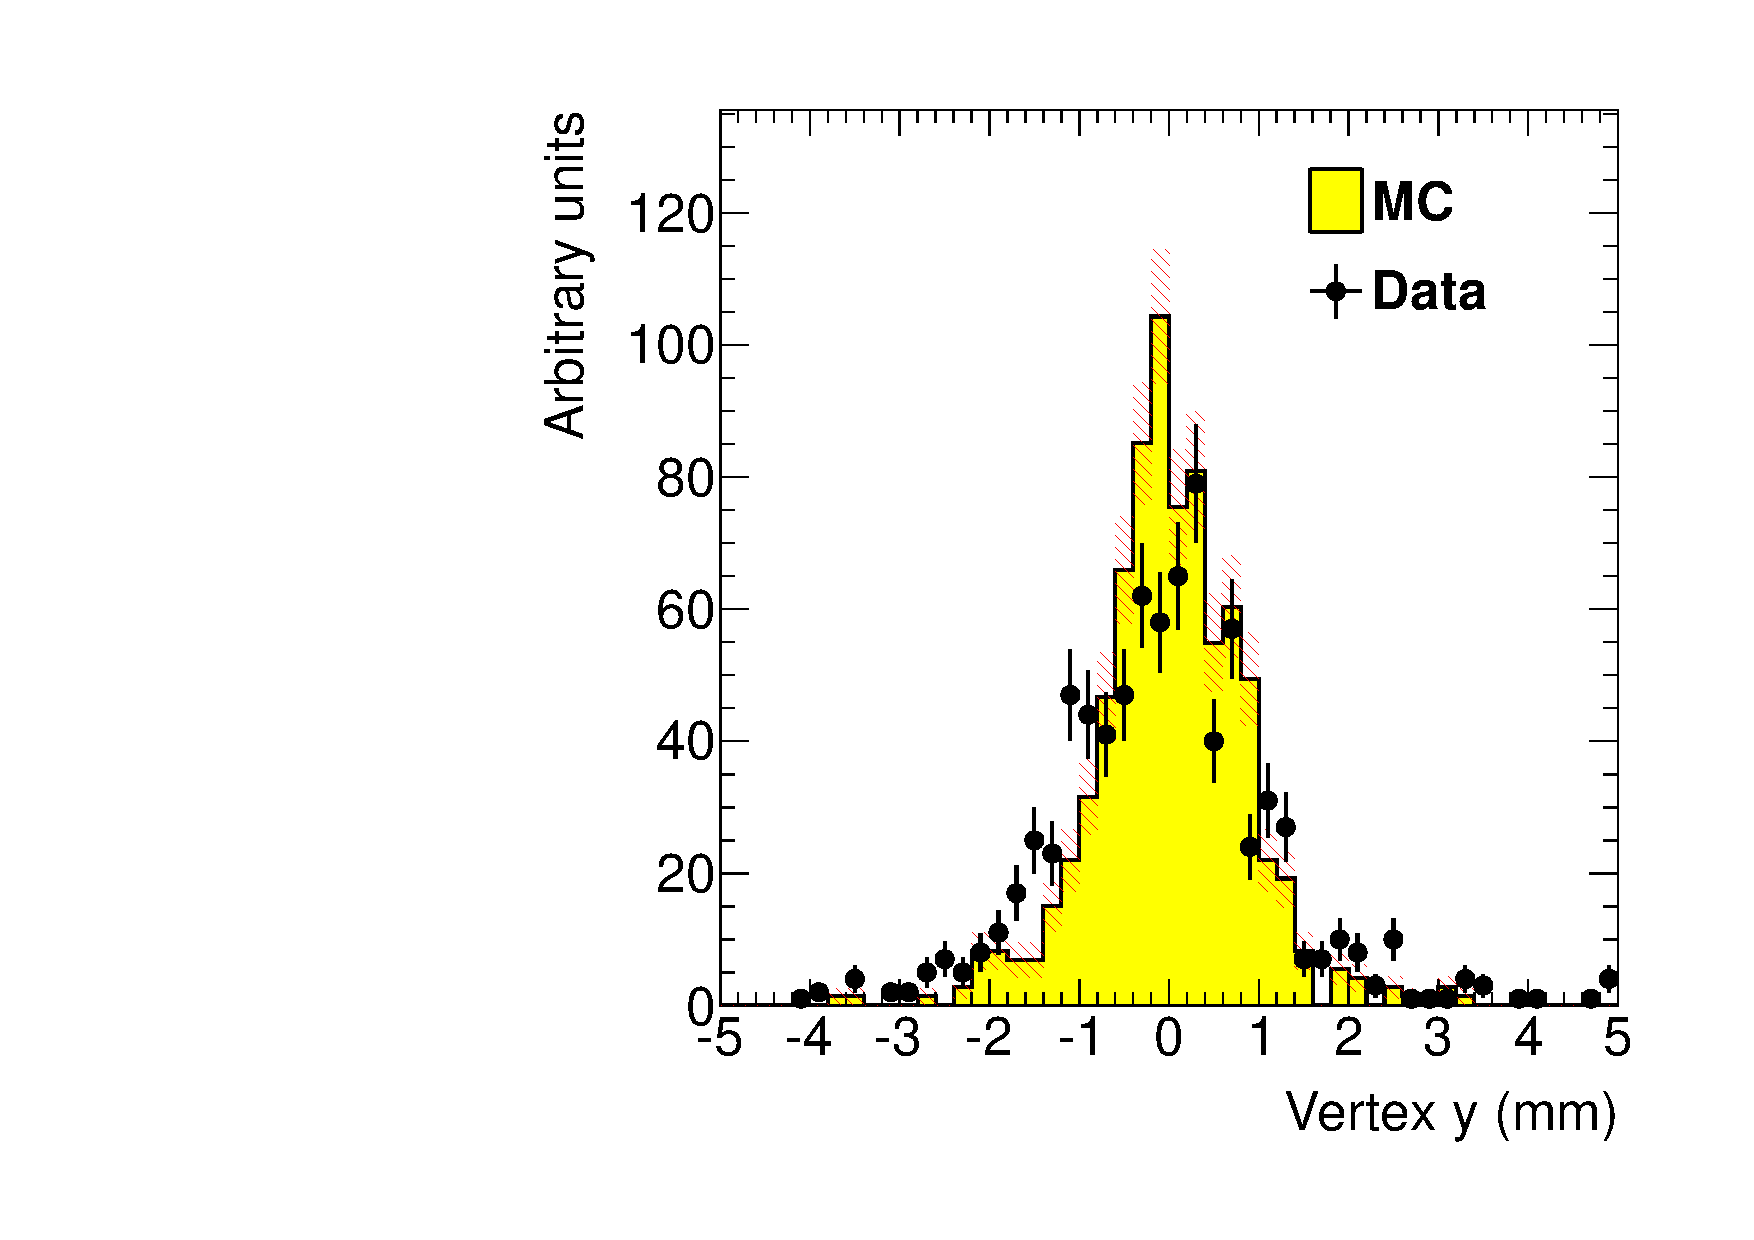
\includegraphics[width=5cm]{figures/h_vtx_fr_z_h_vtx_z_trigsel4hit_pair1351_twotrkfilt-v6-paper}
	\caption{ Vertex position represented by the distance of closest approach of the extrapolated 
	momentum vectors upstream of the PS magnet taking into account the measured fringe field. The 
	overall shift from zero in the x-direction is due to a 30~mrad rotation of the SVT with respect to the 
	beam line.}
	\label{fig:vtx_pos}
\end{figure*}
}
\end{center}
%While the tails of the vertex distribution expected in electron beam running is not accessible here the 
%fact that the core is relatively well described provides confidence of the description of the amount of 
%material and the model used for simulating multiple scattering in the target.  
%These are crucial for benchmarking the HPS \Aprime{} physics reach since both the mass and vertex 
%resolution that determine the sensitivity are limited by multiple scattering.






\subsection{ECal Performance}
\label{sec:ecal_calibration}

%step Of 442 modules, 39 were disabled or disconnected and were not read out by the DAQ. 13 of these were not read out because of a shortage of FADC readout boards (see Sec.~\ref{sec:fadc}).The remainder either had no HV bias on the APD, or were disabled in the FADC software due to noise. In the data, we identified two types of abnormal channels. One FADC was not sending trigger signals correctly, resulting in low efficiency. This affected the 13 channels read out by that FADC. 5 channels were diagnosed as noisy because they  had a high incidence of hits out of coincidence with the trigger. A large number of channels were originally misidentified as noisy because they had much higher hit occupancy than neighboring channels. Gain calibration shows that these channels have high gain (and thus lower energy threshold) but are otherwise normal. The abnormal channels were ignored in analysis in order to simplify comparison with Monte Carlo. This leaves 385 useful channels---87\% of the ECal.

The integrated pulse of the each channel was converted to energy by first 
subtracting the pedestal and then applying a conversion factor to convert ADC counts to energy. 
The pedestals are measured using special runs where each trigger records 100 samples of signals from 
the APDs with 4~ns between each sample. The pedestals were extracted from the 
part of the window before the actual hit in the calorimeter. After subtracting the pedestal, modules with 
integrated pulse above a threshold are clustered using a simple algorithm similar to the one deployed 
for the trigger (see Sec.~\ref{sec:trigger}). Due to the high effective readout threshold of $73$~MeV the 
average number of modules in a cluster was $\sim 3$ and the simple clustering algorithm worked well 
for reconstruction of the detected shower energy. An average noise level of approximately 15~MeV 
was measured in special pedestal runs. 

The ratio of the ECal cluster energy $E$ to the momentum $p$ of a matched track in the SVT was used 
to determine the conversion factors from ADC counts to energy. To compare data and simulation, all 
inoperable or noisy channels in the SVT and ECal was disabled in both data and simulation; any 
efficiency or bias that affect the data should be reflected in the simulation. 
%Furthermore, a conversion factor calibration is performed to equalize the gains of  each channel.  simulation to those observed in data by comparing .  The ``weighted $E/p$'' for each crystal is computed, 
representing the average $E/p$ for clusters that include the crystal
% $\frac{\sum_j w_{j,i}}{\sum_j\frac{P_j}{E_j}w_{j,i}}$.
Iteratively, conversion coefficients for each module is adjusted until the $E/p$ ratio in data and 
simulation are similar. The distribution of the $E/p$ ratio in data and simulation can be seen in 
Fig.~\ref{fig:gains}. 
{\small
\begin{figure}[]
\begin{center}
	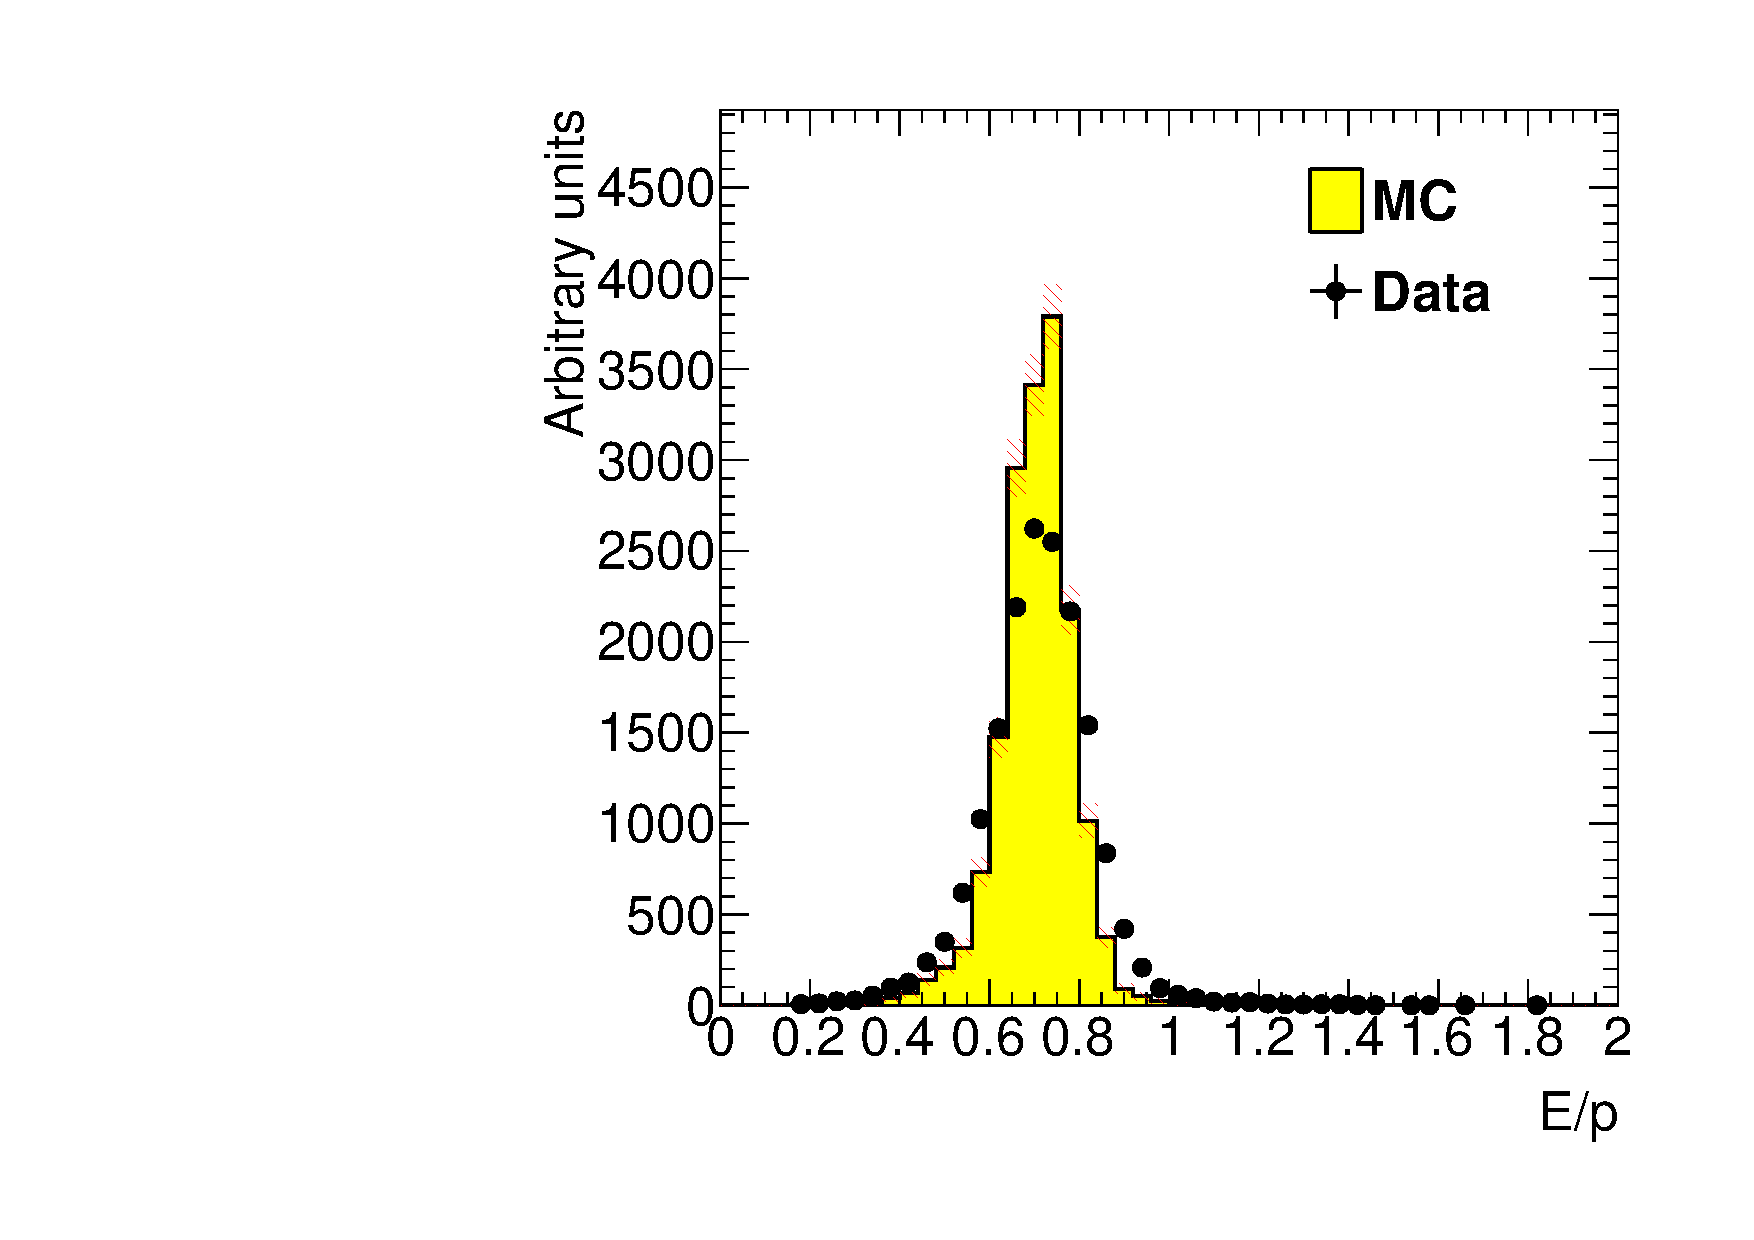
\includegraphics[width=7cm]{figures/h_ep_data_0_h_ep_MC_0_dataMC_1351-v6-v6gains_2-trig-top-cl600reg0.pdf}
	\caption{The ECal energy over track momentum ratio comparing data and simulation} 
	\label{fig:gains}
\end{center}
\end{figure}
}
The peak position of the distribution indicates the sampling fraction of the ECal, 
the fraction of the incident particle energy measured in the cluster. The width and tails of the distribution 
in data indicates imperfect calibration and noise of the ECal modules. This level of calibration and the 
agreement with simulation was found to be sufficient for the multiple scattering analysis using 
normalized event rates described in Sec.~\ref{sec:mcs}.

%These gains can then be used to convert from the ADC counts reported by the FADC in each channels to the energy deposited in the crystals. In order to find the energy of the incident particle one also needs to know the  the fraction of incident energy that is deposited in the cluster or "sampling fraction". 
%The sampling fraction is parameterized from simulation that show that it is approximately 0.9 for the ECal. The weighted $E/p$ shown in Fig.~\ref{fig:gains} is an approximate measurement of the sampling fraction of that part of the ECal but is position- (somewhat smaller at the edges) and energy-dependent because of the high readout thresholds (explaining the low value compared to 0.9). Since the sampling fraction is not needed to normalize event rates it was not applied in the multiple scattering analysis in Sec.~\ref{sec:mcs}.




\subsection{Trigger Performance}
The trigger and DAQ integrate pulses from the ECal modules differently to measure the energy 
deposited in the each crystal. The trigger integrates the pulse using a time-over-threshold window, and 
the DAQ readout integrates using a fixed-size window (5 samples before and 30 samples after a 
threshold crossing). For every event, the trigger reports the trigger decision as a bit mask (top half, 
bottom half or both) and the time the trigger fired. The trigger performance was studied by simulating the 
trigger for each event and comparing to how the events were actually triggered.
First, we simulate the FADC readout board to convert from readout hits (with fixed-size window 
integration) to trigger hits (time-over-threshold integration). Secondly, the CTP clustering 
algorithm and the trigger decision is simulated before we compare the trigger decision and trigger time 
to what was reported by the actual trigger. To eliminate trigger bias, we use a tag and probe method. To 
study the trigger performance in one half of the ECal, we select events which triggered the other half 
and where there was exactly one probe cluster in the ECal half under study. We then measure trigger 
efficiency as the fraction of tagged events that fired the trigger in the probe half as a function of the 
probe cluster energy, shown in Fig.~\ref{fig:turnon}. As a cross-check, the turn-on from the trigger 
threshold was measured to be 1280 in units of ADC counts as expected. The threshold was not 
perfectly sharp because of uncertainties in the conversion from readout to trigger hits described 
above, but based on comparisons with simulation we found that the trigger worked exactly as 
specified.
\begin{figure}[ht]
\begin{center}
{\small
	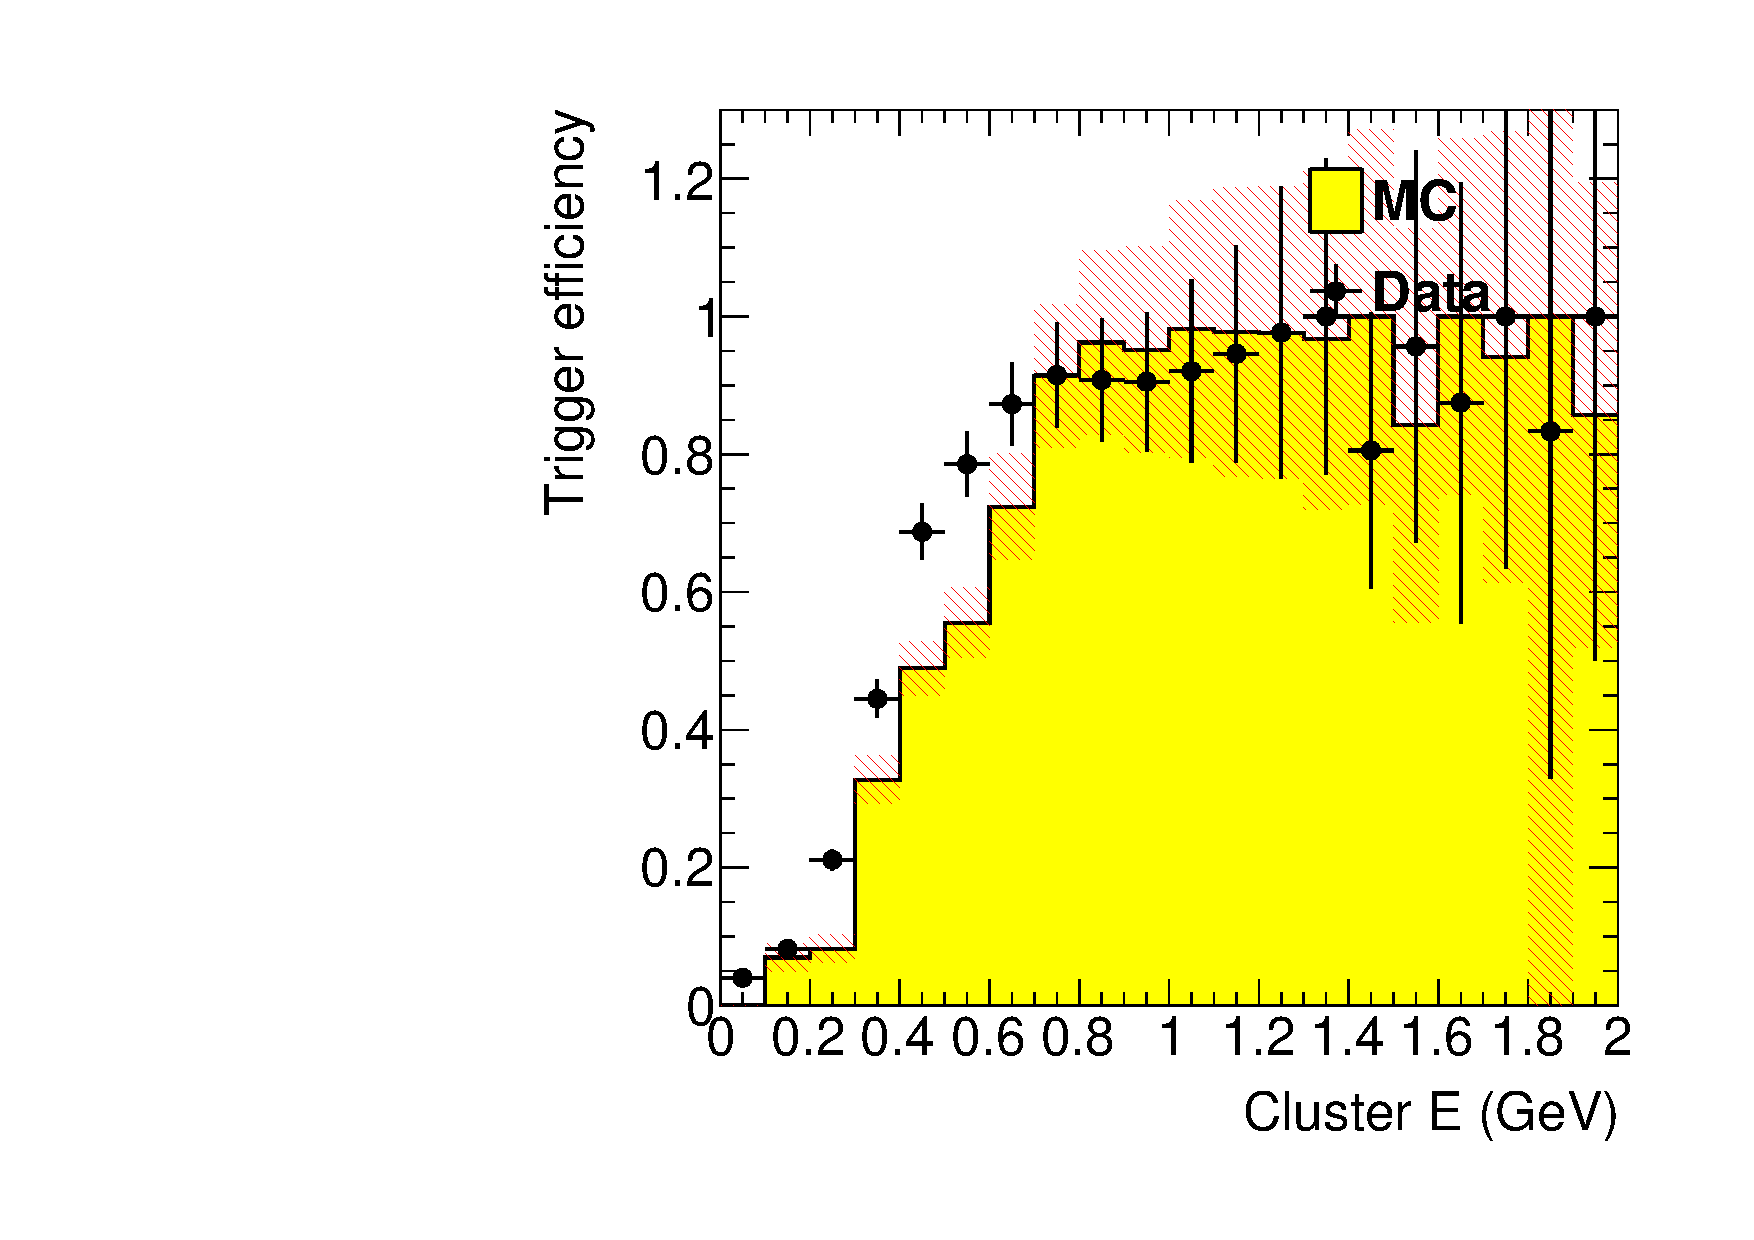
\includegraphics[width=7cm]{figures/h_cl_E_probedata_eff_h_cl_E_probeMC_eff_dataMC_1351-v7-trig-tagBot.pdf}
	\caption{Trigger efficiency in both halves of the ECal for data and simulation as a 
	function of cluster energy.}
\label{fig:turnon}
}
\end{center}
\end{figure}
The trigger turn-on is slow and reaches an uneven plateau just below 1~GeV for two reasons;  
gain variations between different crystals lead to the threshold variations and the nonlinearity of 
the time-over-threshold integral means that the effective threshold is higher for clusters that span 
multiple crystals. The effective trigger threshold is therefore dependent on position and energy of 
the particle as well as cluster multiplicity. 
%Overall the trigger appears to have functioned exactly as intended. 
%Changes planned for physics running (constant integration window and per-crystal gain calibration 
%constants for the trigger) will solve both of the issues that led to threshold variations in the Test run.








%%%%%%%%%%%%%%%%%%%%%%%%%%%%%%%%%%%%%%%%%%%%%%%%%%


\section{Multiple Coulomb Scattering Distributions}
\label{sec:mcs}
Occupancies close to the beam create many of the key challenges in the HPS experiment
and determine the limits of sensitivity to low \Aprime{} masses.
These occupancies are dominated by electrons which have multiple Coulomb scattered (MCS) 
to relatively large angles in the target. Because HPS is sensitive to scattering angles far out on the tail of 
the MCS distribution, well beyond the angles important in other experiments, care must be taken
to ensure our simulations are correct in this regime.  

\subsection{Multiple Coulomb Scattering Models}

One of the main goals of the HPS Test was to evaluate the description of the tails of the MCS
to gain further confidence in the expected detector occupancy in the full HPS experiment. 
Previous studies of multiple scattering angles show good agreement with the \moliere{} 
theory~\cite{Moliere:1948zz} for a wide range 
of materials and projectiles~\cite{Attwood:2005zz,Shen:1978ha,Gottschalk1993467}. We have verified 
that the angular distribution $F(\theta)$ in the differential cross section 
$d\sigma = F( \theta) d(\cos\theta) d\phi$ for the \egs{}~\cite{egs5} simulation program show good 
agreement with \moliere{}'s analytical formula as formulated by Bethe~\cite{Bethe:1953va}. 
The small angle approximation was also shown to be in agreement with the theory formulated by 
Gaudsmit and Saunderson~\cite{Goudsmit:1940zza,Goudsmit:1940zz} that is valid for any angle. 
While \egs{} uses the more complex and time consuming \moliere{} 
formula, the default physics list of \geant{} uses the so-called Urban model, an approximation with two, 
continuously joined, functions to take into account 
small and large angle scattering. Due to the explicit function in large angle approximation used by 
\geant{} we expect that \geant{} will overestimate the angular distribution at angles larger than a few 
mrad.


Figure~\ref{fig:schematic_testrun_vs_erun} gives a schematic view of the main differences 
between the photon and electron beam setup. 
The angular distribution of the pair produced electron and positron emerging 
from the converter in the test run has comparable contributions from {\it i)} the pair production angle
and {\it ii)} the MCS of the electron and positron in the converter after production. By measuring the 
scattering rate at several different converter thicknesses we can vary the contribution from MCS 
while the contribution from the pair production angle is constant. This allows us to confirm our model of MCS 
despite the fact that all data was taken with a photon beam.


\subsection{Running Conditions}

Data was taken at three different converter thicknesses with a beam current varying between 
$30-70$~nA, see~Tab.~\ref{tab:currents}.  
\begin{table}[t]
\begin{center}
{\small
\begin{tabular}{|c|c|c|}
\hline
Converter thickness & Duration &  $e^-$ on converter \\
 (\%$X_0$) & (s) & ($\mu$C)    \\   
\hline
%\hline
1.6   & 911 &   24.4 \\ %24385.9     \\ %27 nA
%\hline
0.18   & 2640 &   193.5 \\ % 193508.9  \\  %73 nA
%\hline
0.45  & 2149 &     140.7 \\ %  140709.9  \\ %65.5 nA
%\hline
0    & 1279  &   88.1 \\ %88079.6  \\
\hline
\end{tabular}
}
\caption{Measured integrated currents for the dedicated photon runs.}
\label{tab:currents}
\end{center}
\end{table}
The photon beam line during the test run produced a relatively 
large fraction of pairs 
originating upstream of the converter. This contribution was measured during data taking 
with ``empty'' converter runs i.e. removing the converter but with all other conditions 
the same. 
The upstream background measured in the ``empty'' converter runs was subtracted 
from the other runs, properly normalized using the measured integrated currents.



\subsection{Measured Angular Distributions}

For this analysis, we measure angular distribution of electrons and positrons using the ECal.
Cluster reconstruction was done using the algorithm described in Sec.~\ref{sec:trigger} build 
clusters around seed hits (hits above a ``seed'' energy threshold and with greater energy than any 
neighboring hits), and add all neighboring hits above an ``add'' energy threshold.
Hit energy is calibrated by matching track momentum to cluster energy, as described in Sec.~\ref{sec:ecal_calibration}. The measured angular distribution in the ECal for the three converter thicknesses are shown in Fig.~\ref{fig:ang_distr_data}. 
\begin{figure}[]
\begin{center}
{\small
%	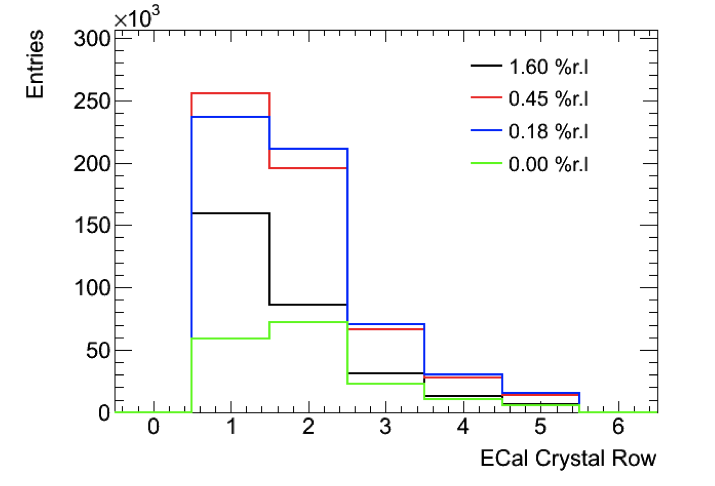
\includegraphics[ width=7cm]{figures/rate_ecalrow_raw.png}
	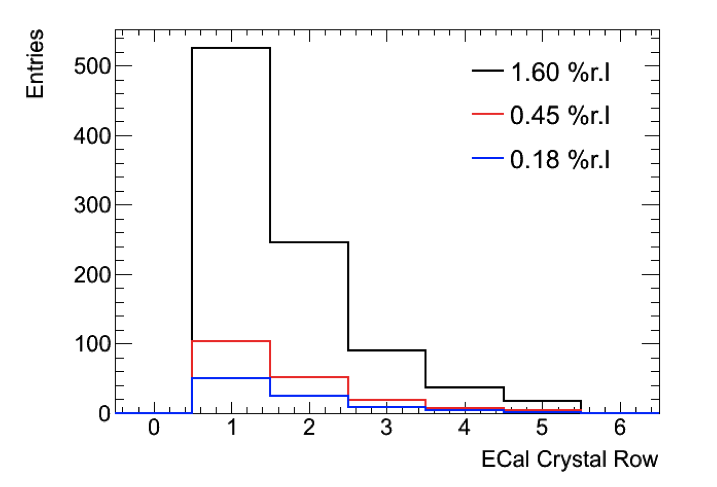
\includegraphics[ width=7cm]{figures/rate_ecalrow_norm_subtr.png}
	\caption{Measured vertical angular distributions after integrated beam current 
	normalization and background subtraction.}
	\label{fig:ang_distr_data}
}
\end{center}
\end{figure}
The data has been normalized to the integrated beam current and the background has been 
subtracted. The background fraction for the there converter thicknesses was 16\%, 52\% and 71\% 
for converter thicknesses of 1.6\%, 0.45\% and 0.18\%, respectively. The background fraction was also 
cross-checked by pointing back tracks reconstructed in the SVT to identify the fraction of tracks not emanating from the converter. 
%This can be seen in Fig.~\ref{fig:extrapol_converter} (bottom) where small 
%satellite peaks at $\pm 10$~mm can be identified as tracks from the upstream background. The angular distribution, after normalization and subtracting the upstream background, are shown in 
%Fig.~\ref{fig:ang_distr_data} (right).  
We also checked that the contribution from photons to our triggered 
sample was less than 2\% (without angular selections which would further reduce the contribution).


These measured angular distributions are compared to simulation to validate 
the modeling of the MCS. \egs{}~\cite{egs5} is used to generate 
the electromagnetic interactions in the converter while \geant{} is used to simulate the particles after the 
converter.  Figure~\ref{fig:ang_distr_dataMC} shows the angular distribution comparing data and 
\egs{} normalized to 1~s of beam at 90~nA beam current with a converter thickness of 1.6\%. 
Reasonable agreement is obtained in the most important region close to the beam. There is a hint of a 
slightly different slope of the data at larger angles; this difference is covered by systematic uncertainties.  
The total rates for each converter thickness is shown in Fig.~\ref{fig:rate_vs_thickness} and summarized 
in Tab.~\ref{tab:ang_distr_dataMC}.
\begin{figure}[]
{\small
	\begin{center}
	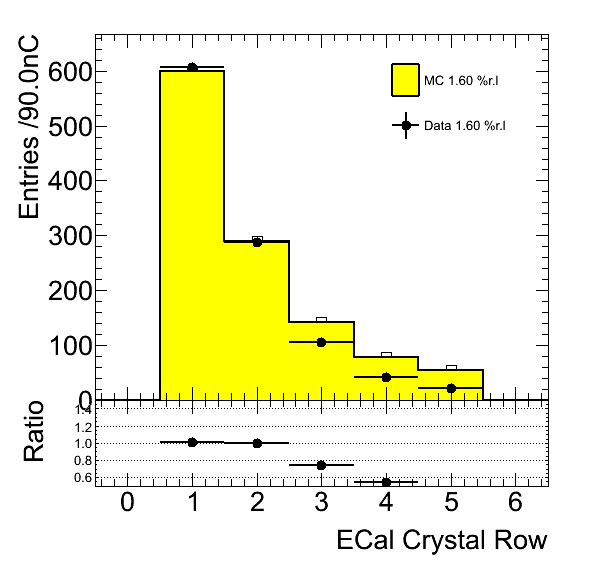
\includegraphics[ width=7cm]{figures/dataMC_1351_Hit_Y_top_norm_bkgsub.png}
	\caption{Comparison between the observed and predicted angular distribution using \egs{} for a 
	converter thickness of 1.6\%. Similar agreement is found for 0.45\% and 0.18\% converter thicknesses. 
	Only statistical uncertainties are shown. }
	\label{fig:ang_distr_dataMC}
\end{center}
}
\end{figure}
\begin{figure}[]
\begin{center}
{\small
	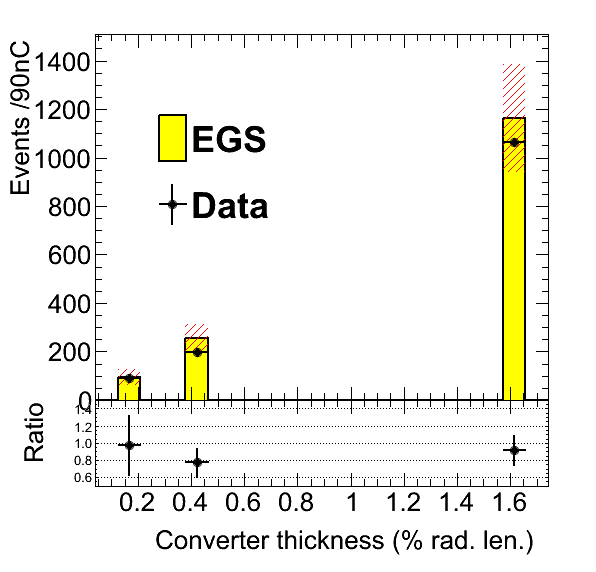
\includegraphics[ width=7cm]{figures/dataMC_egs.png}
	\caption{The measured rate as a function of converter thickness for data and \egs{} simulation 
	of MCS in 	the converter.} 
	\label{fig:rate_vs_thickness}
}
\end{center}
\end{figure}
The total systematic uncertainty was estimated to be between 10-18\% depending on the run including:  
a 5\% uncertainty on the integrated current normalization, alignment of the ECal, uncertainty from the 
background normalization, and limited Monte Carlo statistics.  
\begin{center}
\begin{table}
{\small
\begin{tabular}{|l|c|c|c|}
\hline
Converter (\% r.l.) & 1.60 & 0.45 &	0.18 \\
\hline
EGS5 &	1162 $\pm$ 112 &	255 $\pm$ 28 &	94 $\pm$ 17	\\
\hline
GEANT4 & 2633 $\pm$ 250 & 	371 $\pm$ 38 &	114 $\pm$ 18 \\
\hline
Observed 	& 1064 $\pm$ 2 & 196 $\pm$ 1 &	92 $\pm$ 1 \\						
\hline
\end{tabular}
\caption{ Observed and predicted number of events for 1~s of beam at 90~nA for three different converter 
thicknesses. The uncertainty on the prediction includes systematic uncertainties. }
}
\label{tab:ang_distr_dataMC}
\end{table}
\end{center}

\subsection{Conclusion}
In summary, the accurate modeling of the MCS is fundamental to estimate occupancies and trigger rates 
for HPS. \egs{} predicts the correct angular distribution across all converter thicknesses as expected while 
\geant{}, using the so-called Urban model for multiple scattering overestimates the rates; with the disagreement 
increasing  with larger converter thickness. This preliminary result verifies similar studies [] and gives confidence 
in our modeling of the MCS 
using \egs{} for evaluating the physics reach of HPS.




%%%%%%%%%%%%%%%%%%%%%%%%%%%%%%%%%%%%%%%%%%%%%%%%%%


\section{Summary and Outlook}

%This paper reviewed 
The HPS Test Run experiment, using a simplified version of the apparatus planned for the full HPS experiment in a parasitic photon beam, demonstrated the feasibility of the detector technologies proposed for the HPS silicon tracker, ECal, and data acquisition systems. Performance from each of these subsystems has been shown to be adequate to conduct the full experiment successfully. A measurement of the normalized trigger rates from a photon conversion target confirmed expectations from simulation, giving credance to estimates of the trigger rates and the detector backgrounds expected in electron beam running.  

%The test run achieved the following detector performance:\begin
%{enumerate}
%	\item More than 97\% of SVT channels functioned properly
%	\item Silicon detector signal to noise was 25.5, good enough %to achieve the expected resolutions
%	\item SVT hit time resolution was 2.6 ns, which will permit %background rejection with tight timing cuts 
%	\item SVT hit efficiency was greater than 98\%
%	%\item SVT track reconstruction efficiency was greater than %98\%
%	\item 87\% of ECal crystals functioned properly, with %%defects to be corrected by planned ECal upgrades
%	\item The ECal has been successfully calibrated using SVT %tracks
%	\item The SVT and JLab DAQ were successfully integrated
%	\item The trigger functioned as designed; the FADC trigger 
%rate was tested to greater than 100~kHz
% deficiencies found in test run trigger performance are 
%addressed for the 2014-2015 run
%\end{enumerate}

%While the Test Run successfully allowed us to test many aspects %of the HPS experiment, there were 
%limitations to what could be achieved in some key areas such as %mass resolution and vertexing 
%performance. In particular, the low statistics and lack of 
%resonances or scattered beam electrons prohibits a 
%direct analysis of the momentum 
%and tails of the vertex distribution. However, for both of these %performance parameters, the observed 
%agreement between data and simulation in key distributions 
%supports the performance expected for the 
%proposed experiment. 



%\subsection{Lessons Learned}

%In the process of developing the HPS Test design, it was found 
%that this simple system was capable of 
%delivering a surprising fraction of the physics potential 
%anticipated for the full experiment.  With this in mind, 
%we have proposed a new design for the HPS detector that builds 
%upon the HPS Test , principally 
%by addressing the compromises made for HPS Test to ensure the 
%best possible performance for A$^\prime$ 
%physics within the envelope of the existing beam line layout and %analyzing magnet. For the SVT, 
%this design uses the same sensors, readout chips, and module 
%concept and for the ECal the crystal and 
%detector layout will be identical, retaining the most successful 
%elements of the test run apparatus and addressing the weaknesses %identified during assembly and 
%operation to ensure the success of the 
%experiment. The new SVT layout restores the sixth layer for more %robust tracking, adds acceptance in the 
%deeper layers to increase sensitivity and provides better 
%silicon cooling to improve longevity. Other major 
%updates needed for the full experiment are updates to the SVT 
%electronics and 
%DAQ; improving connectivity and cabling, moving digitization 
%closer to the front-end electronics and 
%updating the data reduction, event handling and trigger 
%synchronization to reach 50kHz 
%trigger rates. 
%This first generation of 
%the full experiment will be ready to take physics data when 
%CEBAF begins operation again in 2014.


\section{Acknowledgements}

%% The Appendices part is started with the command \appendix;
%% appendix sections are then done as normal sections
%% \appendix

%% \section{}
%% \label{}

%% References
%%
%% Following citation commands can be used in the body text:
%% Usage of \cite is as follows:
%%   \cite{key}          ==>>  [#]
%%   \cite[chap. 2]{key} ==>>  [#, chap. 2]
%%   \citet{key}         ==>>  Author [#]

%% References with bibTeX database:

\bibliographystyle{model1-num-names}
%\bibliography{<your-bib-database>}
\bibliography{hps-testrun-nim}

%% Authors are advised to submit their bibtex database files. They are
%% requested to list a bibtex style file in the manuscript if they do
%% not want to use model1-num-names.bst.

%% References without bibTeX database:

% \begin{thebibliography}{00}

%% \bibitem must have the following form:
%%   \bibitem{key}...
%%

% \bibitem{}

% \end{thebibliography}


\end{document}

%%
%% End of file `elsarticle-template-1-num.tex'.
